Section \ref{sec:summary-nts-mtds} highlighted the poor performance of neutron diffusion
methods for calculating neutron fluxes near control rods. Strong neutron absorption in the control
rod region produces a highly anisotropic neutron flux extending some distance outside the control
rod. Neutron transport methods, which retain angular dependence of the neutron flux to various
extents, generally fare better than neutron diffusion methods, which have isotropic diffusion
coefficients. However, neutron transport methods are also generally more computationally expensive,
given the increased dimensionality of the problem from the angular component. Adding an angular
dimension to the existing geometric and neutron energy group dimensions dramatically
increases the problem size and the computational resources necessary to solve the system. Many past
efforts have tried introducing
transport correction techniques to improve neutron flux and multiplication factor estimates in
diffusion-based methods. Other than control rod regions, these techniques may also correct
homogenization errors introduced by spatial homogenization of fuel assemblies and other
structures within a reactor core. They invariably rely on neutron transport methods to generate
transport corrections in the form of corrected diffusion coefficients
\cite{bretscher_computing_1997, scherer_determination_1976, ronen_accurate_2004,
pounders_diffusion_2009, kavenoky_sph_1978}, boundary conditions \cite{davison_influence_1951,
pellaud_extrapolation_1968, fen_modelling_1992}, Eddington factors, or discontinuity factors
\cite{koebke_new_1980}.

In this chapter, I propose a novel hybrid method for improving control rod modeling in neutron
diffusion solvers without spatial homogenization. In essence, the hybrid method involves applying
the $S_N$ discrete ordinates neutron transport method on subregions containing the control rod to
obtain diffusion coefficients which provide pointwise corrections for the diffusion method on the
entire problem domain.

Section \ref{sec:theory} discusses the theoretical background for the hybrid $S_N$-diffusion
method. Section \ref{sec:implementation} provides numerical implementation details of
the hybrid method and its components. Sections \ref{sec:test-case} and \ref{sec:sim-param} describe
the 1-D test cases and several simulation parameters in that context. Section
\ref{sec:prelim-results} discusses the results of the hybrid method applied to the 1-D test cases
with comparisons to higher-fidelity Monte Carlo and $S_N$ neutron transport methods. Lastly,
Section \ref{sec:hybrid-summary} summarizes the key findings in this chapter.

\section{Theory} \label{sec:theory}

The proposed hybrid $S_N$-diffusion method is an iterative method to improve the
accuracy of neutron diffusion solutions in reactor systems with highly anisotropic flux regions
which I will use to model control rods. In this discussion, I focus on the 1-D, $k$-eigenvalue
implementation of the hybrid method. However, my work will extend beyond 1-D in the proposed work.

The discrete ordinates ($S_N$) method for solving the multigroup neutron transport equation
(Eq. \ref{eq:mg-bte}) discretizes the continuous angular directional phase space into a finite
number of discrete angular intervals (ordinates). The set of distinct direction variables
$\hat{\Omega}_n$ representing the discrete ordinates is typically chosen in conjunction with a
compatible quadrature set to replace integrals across continuous solid angles
$\hat{\Omega}$ with quadrature approximations. The multigroup, discrete ordinates ($S_N$
approximation) form of the Cartesian 1-D, $k$-eigenvalue neutron transport equation with the
Gauss-Legendre quadrature set is:
%
\begin{align}
  \mu_n \frac{d}{dx}\Psi_g(x, \mu_n) + \Sigma_{t,g}(x)&\Psi_g(x, \mu_n) -
\sum^G_{g'=1} \sum^N_{n'=1} \sum^L_{l=0} \frac{\left(2l+1\right)}{2}
\Sigma^{g'\rightarrow g}_{s,l}(x) P_l(\mu_{n'} - \mu_n)
w_{n'}\Psi_{g'}(x,\mu_{n'}) \nonumber \\
  &= \sum^G_{g'=1} \frac{\chi_g}{2} \frac{\nu\Sigma_{f,g'}(x)}{k} \phi_{g'}(x) + S_g(x,\mu_n)
  \label{eq:1d-sn}
  \shortintertext{where}
  \mu_n &= \mbox{ cosine of $\hat{\Omega}_n$ relative to the $x$-axis,} \nonumber \\
  \Psi_g(x,\mu_n) &= \mbox{ neutron angular flux along $\mu_n$ in group $g$,} \nonumber \\
%  g &= \mbox{ neutron energy group index, ranging from 1 to G,} \nonumber \\
%  \Sigma_{t,g}(x) &= \mbox{ macroscopic total cross section of neutrons in group $g$,} \nonumber \\
  G &= \mbox{ total number of energy groups,} \nonumber \\
%  n &= \mbox{ discrete ordinate index,} \nonumber \\
  N &= \mbox{ total number of discrete ordinates,} \nonumber \\
  l &= \mbox{ Legendre expansion order,} \nonumber \\
  L &= \mbox{ highest Legendre expansion order,} \nonumber \\
  \Sigma^{g'\rightarrow g}_{s,l}(x) &= \mbox{ $l$-th Legendre moment of the macroscopic
scattering} \nonumber \\
  &\ \ \ \ \mbox{ cross section from group $g'$ to $g$,} \nonumber \\
  P_l &= \mbox{ Legendre polynomial of degree $l$,} \nonumber \\
  w_{n'} &= \mbox{ $n'$-th quadrature weight,} \nonumber \\
%  \chi_g &= \mbox{ fission neutron spectrum in group $g$,} \nonumber \\
%  \nu &= \mbox{ neutrons produced per fission reaction,} \nonumber \\
%  \Sigma_{f,g}(x) &= \mbox{ macroscopic fission cross section of neutrons in group $g$,}
%  \nonumber \\
  k &= \mbox{ neutron multiplication factor.} \nonumber
%  \phi_{g'}(x) &= \mbox{ scalar neutron flux in group $g$,} \nonumber \\
%  S_g(x,\mu_n) &= \mbox{ external neutron source in group $g$.} \nonumber
\end{align}
%
We can retrieve the neutron scalar flux and current by calculating the 0th and 1st Legendre
moments, respectively, as follows:
%
\begin{align}
  \phi_g(x) &= \frac{1}{2} \int^1_{-1} d\mu\ \Psi_g(x,\mu) = \frac{1}{2} \sum^N_{n=1} w_n
\Psi_g(x,\mu_n)
  \shortintertext{and}
  J_g(x) &= \frac{1}{2} \int^1_{-1} d\mu\ \mu\Psi_g(x,\mu) = \frac{1}{2} \sum^N_{n=1} w_n
\mu_n \Psi_g(x,\mu_n)
\end{align}

The 1-D form of the multigroup $k$-eigenvalue neutron diffusion equations (Eq. \ref{eq:mg-diff})
is:
%
\begin{align}
  -\frac{d}{dx} D_g(x) \frac{d}{dx} \phi_g(x) + \Sigma_{t,g}(x) \phi_g(x) &= \sum^G_{g'=1}\left[
  \Sigma_s^{g'\rightarrow g}(x)\phi_{g'}(x) + \chi_g\frac{\nu\Sigma_{f,g'}(x)}{k}
  \phi_{g'}(x)\right] + S_g(x)
  \label{eq:1d-diff}
  \shortintertext{where}
    D_g(x) &= \frac{1}{3 \Sigma_{tr}(x)} \nonumber \\
           &= \mbox{ isotropic neutron diffusion coefficient for group }g. \nonumber
\end{align}

\subsection{Spatially Varying Diffusion Coefficients} \label{sec:svdc}

The conventional approach for determining diffusion coefficients for each subregion involves
running a high-fidelity neutron transport simulation to tally region-wide estimates of the neutron
transport cross section. The transport cross section formulation is derived from the $P_1$
approximation of the neutron transport equation with isotropic sources \cite{bell_nuclear_1970}.
Essentially, each defined subregion has a constant diffusion coefficient value. However, as
discussed in Section \ref{sec:summary-nts-mtds}, the neutron diffusion
equation is only valid in regions of high scattering-to-removal ratios with, at most, linearly
anisotropic scattering and small flux gradients. These conditions do not hold near or within
control rods, near interfaces of neighboring materials with highly dissimilar neutronic properties,
and in materials with significant scattering contributions from light nuclei.

In the hybrid $S_N$-diffusion method, I propose replacing the conventional $P_1$-based
diffusion coefficients with an alternate formulation that incorporates pointwise corrections
to the neutron diffusion flux solution from the $S_N$-derived flux solution as follows:
%
\begin{align}
  D^s_g(x) &= -J^{tr}_g(x)\bigg/\frac{d\phi^{tr}_g(x)}{dx}. \label{eq:svdc}
\end{align}
%
where $D^s$ is the \glspl{SVDC}, and the $tr$ superscript denotes the transport-computed neutron
current and scalar flux solutions from the $S_N$ method.
The basic form of this equation is Fick's first law of diffusion. The result is a diffusion
coefficient variable that continuously varies in space from point to point except at dissimilar
material interfaces. \glspl{SVDC} provide pointwise corrections to closely match the diffusion flux
solution to the $S_N$ flux solution.

Eq. \ref{eq:svdc} is identical to Ronen's \cite{ronen_accurate_2004} and Pounders \& Rahnema's
\cite{pounders_diffusion_2009} formulations for space-dependent diffusion coefficients in Eq.
\ref{eq:ronen} and Eq. \ref{eq:emp}, respectively. In comparison with
the Ronen method, our approaches differ in how $\phi_{tr}$ and $J_{tr}$ are obtained. Starting with
a standard neutron diffusion calculation, the Ronen method applies an analytically derived
transport operator on every iteration to calculate a new estimate of $J_{tr}$ using the $\phi$
solution from the previous iteration. The main difficulty for the Ronen method lies in deriving the
transport operators which has been achieved for only simple 1-D geometries thus far.

For the \textit{empirical method} by Pounders \& Rahnema, their diffusion coefficients are
piecewise-constant and they assumed a priori knowledge of the reference flux solution.
Pounders \& Rahnema \cite{pounders_diffusion_2009} demonstrated the effectiveness of applying
pointwise corrections derived from analytical or Monte Carlo reference flux solutions. Compared
with conventional $P_1$-based out-scatter and flux-limited approximations of the diffusion
coefficient, their diffusion coefficients showed superior agreement
with the reference flux solutions. They recognized that volume averaging within each mesh element
for piecewise-constant diffusion coefficients introduces some truncation error if the flux is
non-linear within the mesh element. This design choice may be due to an intention to retain the
diffusion coefficient as a constant in the $\frac{d}{dx}D\frac{d\phi}{dx}$ term of the neutron
diffusion equation (Eq. \ref{eq:1d-diff}).

Unlike their approach, the \gls{SVDC} formulation in Eq. \ref{eq:svdc} allows for continuously
varying diffusion coefficients to reduce truncation error. In practice, the discretization order of
\gls{SVDC} variables in a numerical calculation would be the same as the discretization order of
the reference flux solution. This formulation introduces a minor change to the finite difference
implementation of the 2nd-order diffusion term to handle spatial derivatives of the
diffusion coefficient. However, the finite element implementation sees no change as the 2nd-order
diffusion term is commonly treated with integration-by-parts to reduce it to a 1st-order
differential term with no derivatives of the diffusion coefficient. Refer to Section
\ref{sec:implementation} for key numerical implementation details of a finite difference neutron
diffusion solver with support for handling \glspl{SVDC}.

For the rest of Section \ref{sec:svdc}, I will show how the \glspl{SVDC} may differ from the
conventional $P_1$-based diffusion coefficient before presenting further details of the hybrid
$S_N$-diffusion method in Section \ref{sec:theory}.

\begin{figure}[htb!]
  \centering
  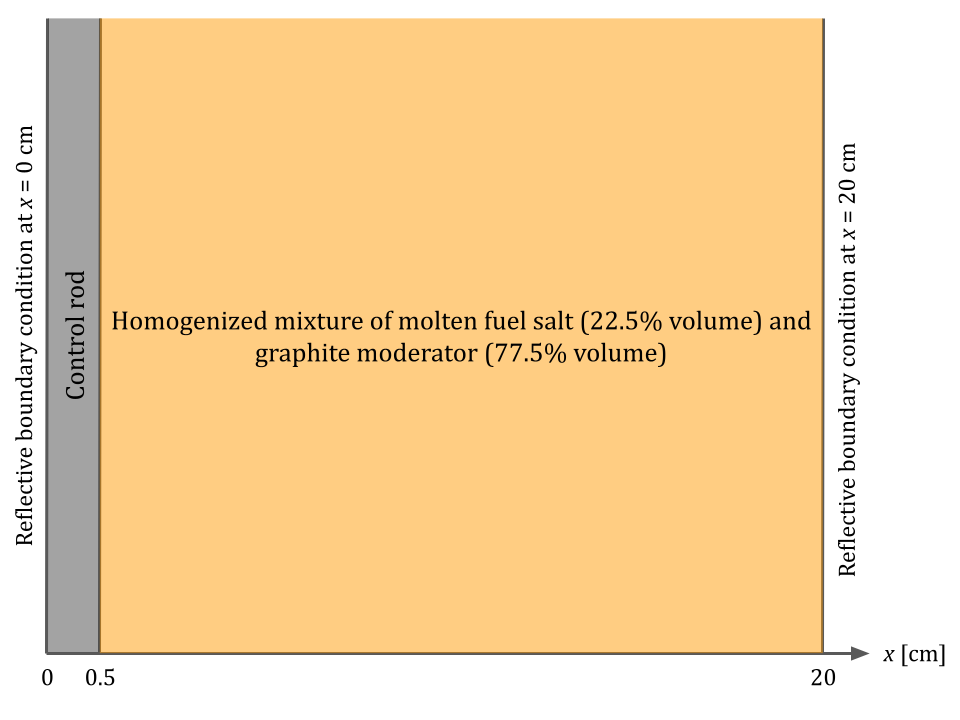
\includegraphics[width=.7\columnwidth]{case-0-geometry}
  \caption{Case 0: A 1-D, two-region system containing a 0.5-cm thick control rod and a 24.5-cm
    thick homogeneous mixture of molten fuel salt and graphite moderator. Reflective boundary
    conditions apply on both ends.}
  \label{fig:case-0-geom}
\end{figure}

\subsubsection{\gls{SVDC} Demonstration with Case 0}

To facilitate the following demonstration of a neutron diffusion calculation with \glspl{SVDC},
consider a 1-D, two-region system (which I will refer to as Case 0 moving forward) consisting of a
highly neutron-absorbing material and a
neutron-multiplying region with reflective boundary conditions on both ends (Figure
\ref{fig:case-0-geom}). I defined the material specifications of the control rod, molten fuel salt,
and graphite moderator based on the material compositions of the \gls{MSRE}
\cite{robertson_msre_1965}. The
homogenized molten fuel salt and graphite regions minimize discrepancies arising from geometrical
heterogeneity. The group constant input data for the diffusion and $S_N$ solvers (e.g., $P_1$-based
diffusion coefficients, cross sections, fission spectra) were sampled at 900 K and generated using
the OpenMC Monte Carlo neutronics software \cite{romano_openmc:_2015}. OpenMC uses the flux-limited
approximation method, developed by Pomraning \cite{pomraning_flux-limited_1984}, to calculate
diffusion coefficients. The condensed
neutron energy spectrum forms two energy groups bounded between $10^{-5}$, $10^0$, and $10^8$ eV.

I solved for the neutron flux in this system using the following set of numerical solvers:
%
\begin{enumerate}
  \item Neutron diffusion solver with $P_1$-based diffusion coefficients generated directly from
    the group constant generation step with OpenMC.
  \item $S_N$ neutron transport solver with $N=8$ and up to 2nd-order Legendre
    moments of the group-to-group neutron scattering cross sections.
  \item Neutron diffusion solver with \glspl{SVDC} generated from the prior $S_8$
    flux solution.
\end{enumerate}
%
I implemented the diffusion solvers using the finite difference method and the $S_N$
solver using the diamond-difference transport sweep method in Python. For
brevity, I defer further numerical implementation details of these solvers to Section
\ref{sec:implementation}.

\begin{figure}[htb!]
  \centering
  \begin{subfigure}[b]{.49\textwidth}
    \centering
    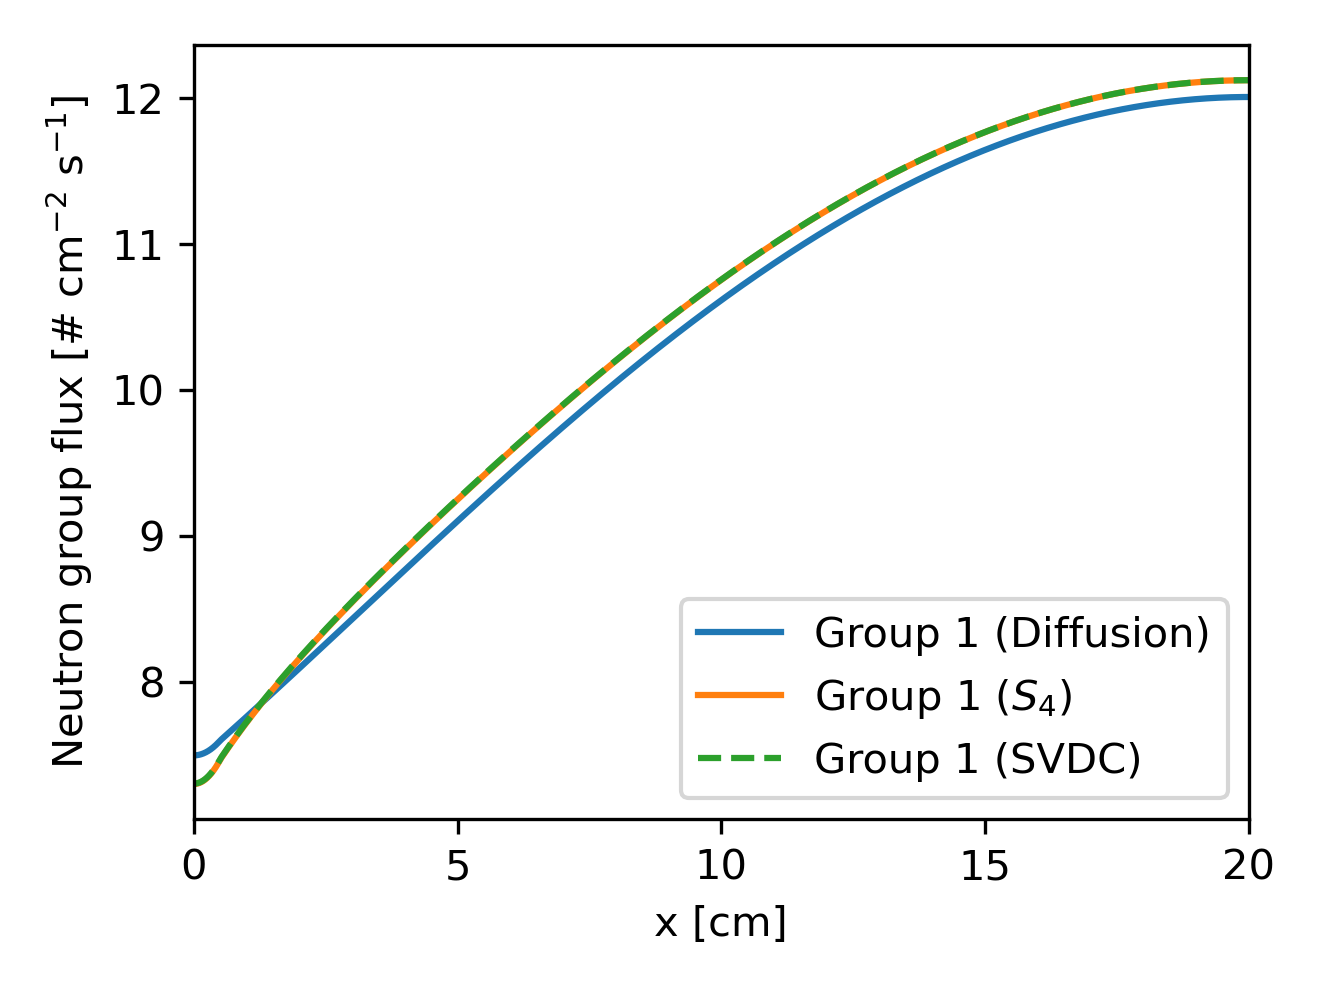
\includegraphics[width=\textwidth]{case-0-group-1-flux}
    \caption{Group 1}
    \label{fig:c0g1flux}
  \end{subfigure}
  \hfill
  \begin{subfigure}[b]{.49\textwidth}
    \centering
    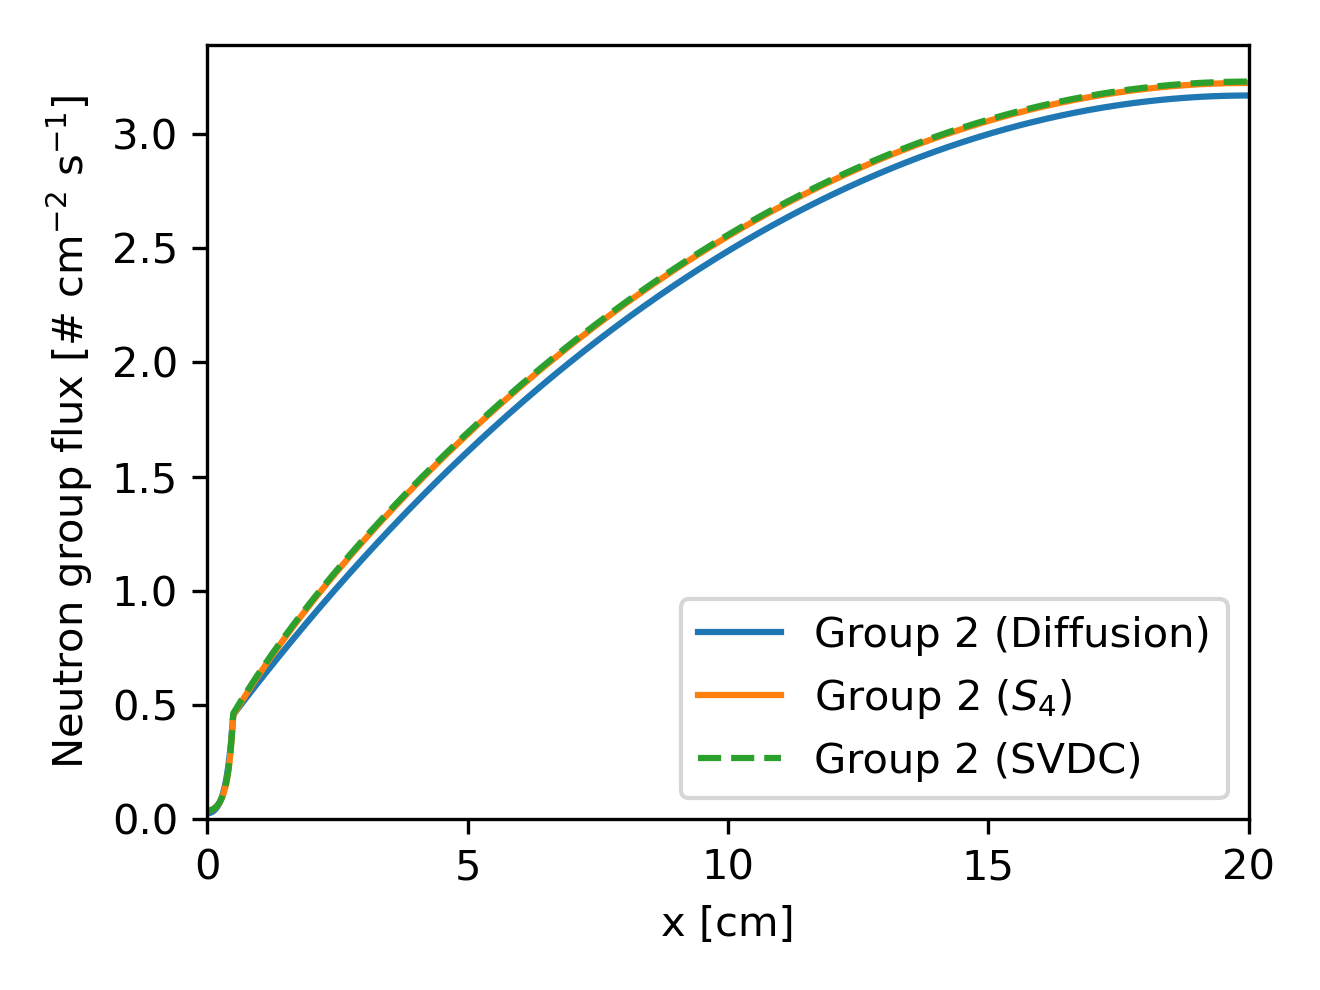
\includegraphics[width=\textwidth]{case-0-group-2-flux}
    \caption{Group 2}
    \label{fig:c0g2flux}
  \end{subfigure}
  \caption{Neutron group 1 and 2 flux distributions from the diffusion, $S_8$, and
  diffusion-\gls{SVDC} solvers for Case 0.}
  \label{fig:c0flux}
\end{figure}
%
\begin{figure}[htb!]
  \centering
  \begin{subfigure}[b]{.49\textwidth}
    \centering
    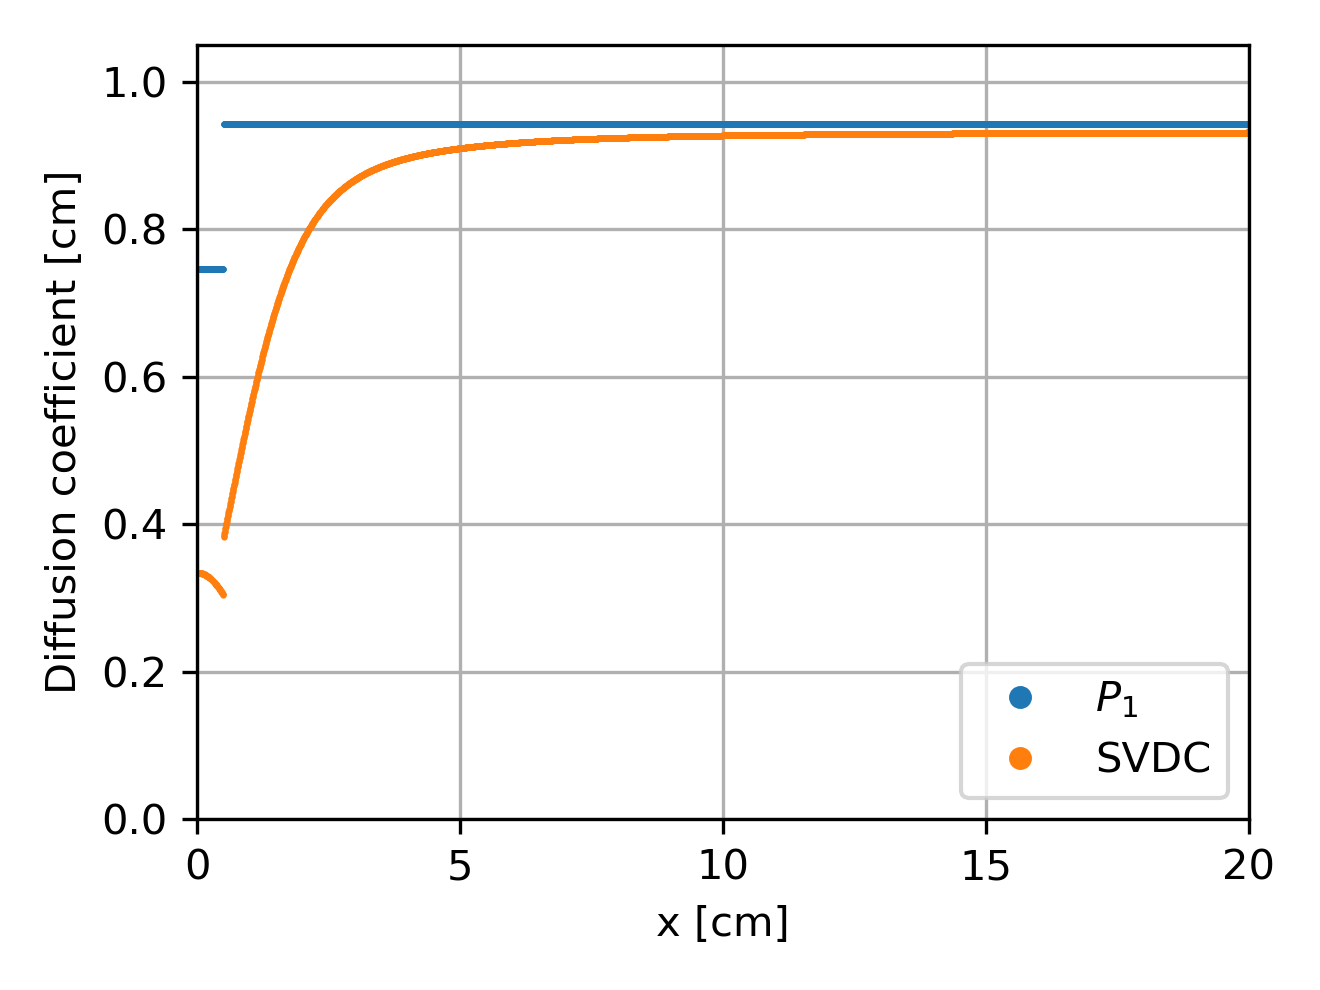
\includegraphics[width=\textwidth]{case-0-group-1-diffcoef}
    \caption{Group 1}
    \label{fig:c0g1diffcoef}
  \end{subfigure}
  \hfill
  \begin{subfigure}[b]{.49\textwidth}
    \centering
    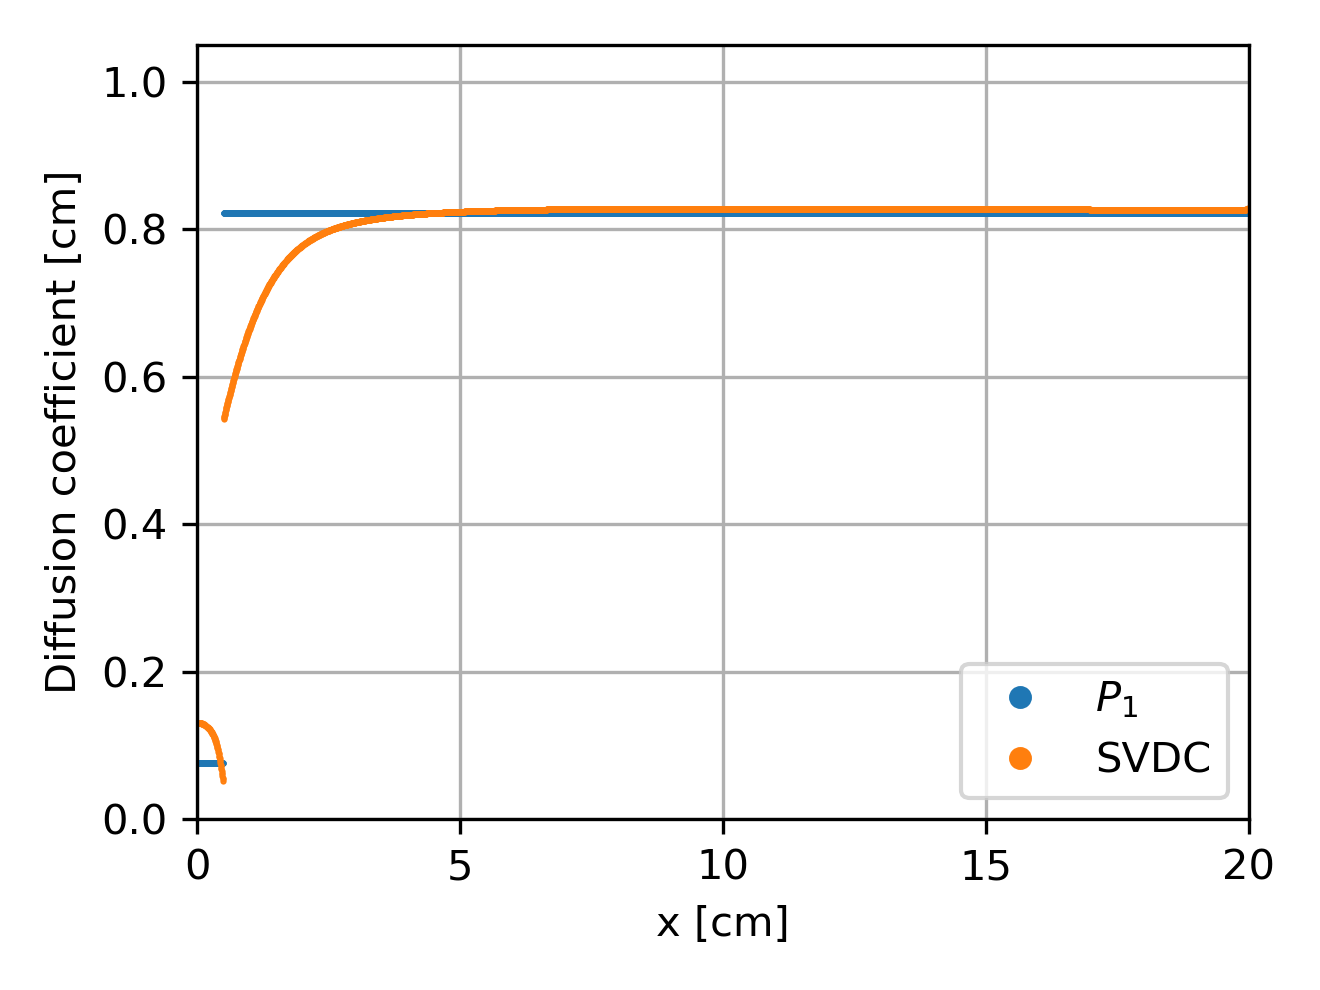
\includegraphics[width=\textwidth]{case-0-group-2-diffcoef}
    \caption{Group 2}
    \label{fig:c0g2diffcoef}
  \end{subfigure}
  \caption{$P_1$-based diffusion coefficient and \gls{SVDC} spatial distributions
  for Case 0.}
  \label{fig:c0diffcoef}
\end{figure}

Figure \ref{fig:c0flux} shows the group 1 and 2 neutron fluxes from the diffusion-$P_1$, $S_8$, and
diffusion-\gls{SVDC} solvers with a uniform mesh size of 0.005 cm. I omitted the OpenMC flux
solution because this exercise aims to demonstrate the effectiveness of \glspl{SVDC}
in reproducing an $S_N$-derived flux solution. As expected, the diffusion-$P_1$ flux solution
deviates from the $S_8$ flux solution, while the diffusion-\gls{SVDC} flux solution shows
significantly better agreement with the $S_8$ flux solution. As shown in Table \ref{table:c0k}, the
$k$ estimate from the diffusion-\gls{SVDC} solver is also closer to the $k$ estimate from the
$S_8$ solver than the diffusion-$P_1$ solver.

\begin{table}[tb!]
  \centering
  \caption{Multiplication factor $k$ estimates from the diffusion-$P_1$, $S_8$, and
  diffusion-\gls{SVDC} solvers and the absolute difference relative to the $S_8$ estimate.}
  \begin{tabular}{l S S}
    \toprule
    Solver type & {$k$} & {$k-k_{S_8}$} \\
    \midrule
    $S_8$ & 0.62736 & {-} \\
    Diffusion-$P_1$ & 0.60890 & -0.01846 \\
    Diffusion-\gls{SVDC} & 0.62750 & +0.00013 \\
    \bottomrule
  \end{tabular}
  \label{table:c0k}
\end{table}

The $P_1$-based diffusion coefficients and \glspl{SVDC} in Figure \ref{fig:c0diffcoef} show good
agreement in the bulk fuel salt region far from the control rod region.
This observation supports the validity of the neutron diffusion method under the conditions
listed at the start of Section \ref{sec:svdc}. Closer to the control rod
region, the \glspl{SVDC} deviate from the $P_1$-based diffusion coefficients because the
prerequisites for diffusion theory are violated.

Another key finding from this study is that the neutron diffusion method with $P_1$-based
diffusion coefficients fails to reproduce the steep $S_8$ flux gradient in the control rod region
for group 1 and in the homogeneous fuel-graphite region adjacent to the control rod region for both
neutron groups. From a purely mathematical perspective, the streaming term in the neutron
diffusion equation requires the lower
\gls{SVDC} values in the absorber-adjacent region to induce steeper flux gradients and match the
$S_8$ flux solution. Given that highly neutron-absorbing materials induce steep flux gradients
around them, we can expect similar trends of \glspl{SVDC} being suppressed relative to
$P_1$-based diffusion coefficients in other systems with control rods. The \gls{SVDC} values within
the highly-absorbing region exhibit significant spatial variation but do not necessarily fall
below the $P_1$-based diffusion coefficients.

Thus far, this method is redundant because it requires a priori knowledge of a reference
analytical flux solution or a highly accurate numerical solution calculated using neutron
transport methods. While existing workflows for diffusion-based methods already require
computationally intensive neutron transport simulations for group constant generation, this
preprocessing step incurs a fixed computational cost through
a series of neutron transport simulations. Compared to \glspl{SVDC}, $P_1$-based diffusion
coefficients behave much more like intrinsic material properties as their definitions are largely
tied to material cross sections. Variations in $P_1$-based diffusion coefficients primarily arise
from changes in the neutron energy spectrum with no direct contribution from proximity to material
interfaces (geometrical heterogeneity). $P_1$-based diffusion coefficients may be generated at
various reactor temperatures and interpolated to model the temperature dependence. Conversely, the
nature of \glspl{SVDC} as empirical, pointwise corrections for the diffusion equation
makes it highly dependent on the neutron flux gradient and susceptible to more significant
variations than region-wide estimates for $P_1$-based diffusion coefficients. \glspl{SVDC} will
likely need to be dynamically generated at every timestep, such as with a two-level iterative
scheme consisting of a $S_N$ neutron transport calculation and a neutron
diffusion calculation. In this case, the required number of neutron transport simulations scales
with the number of reactor simulations. Therefore, \gls{SVDC} generation cannot be adopted as a
one-off preprocessing step. 

Another significant challenge of \glspl{SVDC} and the high-order empirical diffusion coefficients
involves their resolution near neutron flux peaks. The neutron current and flux gradient values in
Eq. \ref{eq:svdc} generally do not reach zero at the same points in space,
resulting in diffusion coefficient values tending to positive or negative infinity when the
flux gradient is close to zero. Pounders \& Rahnema avoided this issue by using
larger mesh sizes to calculate their empirical diffusion coefficients. However, their
remedy contradicts mesh convergence requirements and would worsen flux accuracy in regions with
steep, non-linear fluxes, such as near control rods. I will discuss my approach for investigating
and finding an alternative solution for this issue in Section \ref{sec:devel-hybrid}.

\subsection{Hybrid $S_N$-Diffusion Method} \label{sec:hybrid-method}

In order to reduce the computational cost of the high-level $S_N$ calculation, I propose reducing
the problem domain of the $S_N$ method to a \textit{correction region} containing the control rod
and its vicinity. Consequently, the hybrid $S_N$-diffusion method can retain accurate neutron flux
and current estimates around the control rod region from the $S_N$ method while making significant
computational cost savings by treating most of the reactor geometry with the neutron diffusion
method alone. Henceforth, I will refer to the $S_N$ calculation on the correction
region as the $S_N$ \textit{subproblem} or \textit{sub-solver}. I define the full problem
domain and the correction region as $V_0$ and $V_1$, respectively, where
$V_1\subseteq V_0$. The algorithm for the hybrid $S_N$-diffusion method is as follows:
%
\begin{enumerate}
  \item Start with an initial neutron diffusion calculation in $V_0$ with conventional
    $P_1$-based diffusion coefficients and other standard group constants (e.g., neutron cross
    sections).
  \item Use the neutron diffusion flux estimates in $V_1$ and current estimates along
    $\partial V_1$ as initial and boundary conditions for the $S_N$ sub-solver.
  \item With the $S_N$ sub-solver, calculate an improved neutron flux solution in $V_1$,
    which contains the control rod region and its immediate vicinity.
  \item Calculate \glspl{SVDC} using the $S_N$ flux solution and Eq. \ref{eq:svdc}.
  \item Pass the \glspl{SVDC} to the neutron diffusion solver to replace the conventional
    $P_1$ diffusion coefficients within the $V_1$ while continuing to use $P_1$-based
    diffusion coefficients in the rest of $V_0$.
  \item Start the next iteration by running neutron diffusion calculation with the \glspl{SVDC}
    replacing $P_1$ diffusion coefficients in part or all of $V_1$.
  \item Repeat Steps 2-6 until convergence is reached by meeting pre-defined convergence tolerance
    values.
\end{enumerate}
%
Figure \ref{fig:algorithm} shows a visual flowchart of the same hybrid method algorithm.

\begin{figure}[b!]
  \tikzstyle{every node}=[font=\small]
  \centering
  \begin{tikzpicture}
    \node (1) [object] {\textbf{Perform initial neutron\\diffusion calculation in $\bm{V_0}$}};
    \node (2) [process, below of=1, yshift=-1.8cm]
      {\textbf{Calculate incident flux boundary conditions along\\$\bm{\partial V_1}$ for $S_N$ calculation}};
    \node (3) [process, below of=2, yshift=-1.5cm]
      {\textbf{Perform $\bm{S_N}$ calculation\\in $\bm{V_1}$ for $\bm{\phi^{tr}_i}$ \& $\bm{J^{tr}_i}$}};
    \node (4) [process, below of=3, yshift=-1.5cm]
      {\textbf{Calculate $\bm{D^s_i}$ using Eq. \ref{eq:svdc}}};
    \node (5) [process, below of=4, yshift = -1.5cm]
      {\textbf{Perform neutron diffusion\\calculation in $\bm{V_0}$ using $\bm{D^s_i}$ in $\bm{V_1}$}};
    \node (6) [decision, below of=5, yshift = -1.8cm]
      {\textbf{Convergence\\check}};
    \node (7) [object, below of=6, yshift = -2cm]
      {\textbf{Final $\bm{\phi}$ and $\bm{k}$\\solutions obtained}};
    \draw [arrow] (1) -- node[anchor=east] {$\bm{\phi_0, J_0}$} (2);
    \draw [arrow] (2) -- node[anchor=east] {$\bm{\Psi^-}$ \textbf{along} $\bm{\partial V_1}$} (3);
    \draw [arrow] (3) -- node[anchor=east] {$\bm{\phi^{tr}_i, J^{tr}_i}$} (4);
    \draw [arrow] (4) -- node[anchor=east] {$\bm{D^s_i}$} (5);
    \draw [arrow] (5) -- node[anchor=east] {$\bm{\phi_i, J_i$}} (6);
    \draw [arrow] (6) -- node[anchor=east] {\textbf{Yes}} (7);
    \draw [arrow] (6) -- ([shift={(2cm,0cm)}]6.east)-- node[anchor=west] {\textbf{No}} ([shift={(0.5cm,0cm)}]2.east)--(2);
  \end{tikzpicture}
  \caption{Algorithm flowchart for the hybrid $S_N$-diffusion method.}
  \label{fig:algorithm}
\end{figure}

\subsubsection{$S_N$ Subsolver Boundary Conditions \& Buffer Zone}

The main challenge lies in determining appropriate boundary conditions for the $S_N$ subproblem.
Given that we want to limit the coverage of $V_1$ to the control rod region and its
immediate vicinity, $V_1$ should be sufficiently smaller than $V_0$, but large enough to capture
anisotropies in the flux due to the control rod. As a consequence, the boundaries $\partial V_1$ 
lie well within $V_0$. Crucially, there is currently no feasible method of generating
accurate boundary fluxes for an $S_N$ solver from a neutron diffusion flux solution. In 1-D, the
standard one-group $S_N$ method requires N/2
incoming boundary flux parameters per boundary mesh point for the N/2 neutron angular fluxes
flowing into $V_1$. The neutron diffusion method can produce at most one independent
incoming flux parameter per mesh point; this parameter is the neutron forward/backward current in
the $P_1$ approximation defined as:
%
\begin{align}
  J_{g,\pm} &= \frac{\phi_g}{4} \mp \frac{D_g}{2}\frac{d\phi_g}{dx} \label{eq:p1-j}
  \shortintertext{where}
  J_{g,\pm} &= \mbox{ neutron forward/backward current of group }g. \nonumber
\end{align}
%
Without additional information, the next best estimate is a uniformly
isotropic transmission of angular flux, i.e., all N/2 incoming angular fluxes $\Psi$ are equal in
magnitude. This is a good assumption far from the control rod, but will not produce accurate
fluxes if the boundary is too close to the control rod. This type of boundary condition is similar
to the white boundary condition, which describes the uniformly
isotropic reflection of particles at a boundary, except this case involves transmission rather than
reflection. Isotropic flux transmission at $x$ can be expressed mathematically for forward angular
fluxes as:
%
\begin{align}
  \sum^N_{n=N/2+1}w_n\mu_n\Psi(x,\mu_n) =& J_{+}(x) && (\mu_n>0) \nonumber \\
  \Psi(x,\mu_n)\sum^N_{n=N/2+1}w_n\mu_n =& J_{+}(x) && (\because \mbox{isotropic transmission})
  \nonumber \\
  \Psi(x,\mu_n) =& J_{+}(x)\Bigg/\sum^N_{n=N/2+1}w_n\mu_n
\end{align}
%
and backward angular fluxes as:
%
\begin{align}
  \sum^{N/2}_{n=1}w_n\mu_n\Psi(x,\mu_n) =& J_{-}(x) && (\mu_n<0) \nonumber \\
  \Psi(x,\mu_n)\sum^{N/2}_{n=1}w_n\mu_n =& J_{-}(x) && (\because \mbox{isotropic transmission})
  \nonumber \\
  \Psi(x,\mu_n) =& J_{-}(x)\Bigg/\sum^{N/2}_{n=1}w_n\mu_n \label{eq:sn-psi-j}
\end{align}
%
These boundary conditions for the $S_N$ sub-solver will generally yield some deviations in the
$\phi$ distributions since neutron fluxes in realistic reactor systems are at least slightly
anisotropic in most of the domain. However, in my preliminary investigations, the influence of
boundary conditions on the ratio $J$ and $\frac{d\phi}{dx}$ does not extend far from the boundaries
in optically thick media due to the strong scattering (e.g., graphite or molten salt) or
absorption effects (e.g., control rod). In the bulk regions far from the boundaries, the
scattering and absorption effects have the most significant influence on the flux. I observed that
the \glspl{SVDC} generated with the $S_N$ sub-solver within $V_1$ were accurate everywhere except
near $\partial V_1$. Therefore, $V_1$ must be large enough to provide transport corrections
through the \glspl{SVDC} and accommodate inaccurate \glspl{SVDC} near
$\partial V_1$. The inaccurate \glspl{SVDC} should then be discarded in favor of using
$P_1$-based diffusion coefficients as in the rest of $V_0$ not covered by $V_0$. The
subsequent neutron diffusion calculation with this mix of \glspl{SVDC} and $P_1$-based diffusion
coefficients should provide more accurate $\phi$ and $k$ estimates than a conventional
neutron diffusion calculation.

%To resolve this issue, I posit the following hypothesis: \textit{If there exists a highly
%neutron-absorbing control rod region within the $S_N$ subproblem domain $V_1$ and the $S_N$
%subproblem boundary $\partial V_1$ lies several neutron mean free paths away from this
%region, the \gls{SVDC} values calculated near the control rod region (using the $S_N$ sub-solver
%with isotropic hemisphere boundary conditions) will tend to the actual flux gradient solution
%(using a reference $S_N$ calculation across the entire problem domain $V$).} In other words,
%suboptimal boundary conditions may induce inaccurate \gls{SVDC} values near the $\partial
%V_1$ subdomain boundaries, but the \gls{SVDC} values further from $\partial V_1$ are
%accurate and very weakly dependent on the boundary conditions. These inaccurate \gls{SVDC} values
%close to $V_1$ may be discarded in favor of the default $P_1$-based diffusion coefficients.
%I will refer to the region containing these discarded values as the \textit{dead zone} or
%$V_2$, where $V_2 \subset V_1 \subseteq V_0$.

\subsubsection{Hybrid Method Verification with Case 0}

In this subsection, I revisit Case 0
(Figure \ref{fig:case-0-geom}) to test my hypothesis and demonstrate the hybrid $S_N$-diffusion
method. Once more, I defer general numerical implementation details to
Section \ref{sec:implementation}.

In Section \ref{sec:svdc}, the \gls{SVDC} generated from the reference $S_8$ calculation exhibited
significant spatial variations attributed to the presence of the control rod, as shown in Fig
\ref{fig:c0diffcoef}. The group 1 and 2 \gls{SVDC} values approach asymptotic values near the
corresponding group 1 and 2 $P_1$-based diffusion coefficient values near $x=15$ cm and $x=5$ cm,
respectively. Therefore, the $V_1$ should, at minimum, cover the domain between $x=0$ cm and
$x=15$ cm. Allowing for a buffer region for inaccurate \glspl{SVDC} near $\partial V_1$, I
defined $V_1$ to span from $x=0$ cm to $x=17.5$ cm.

I set up the hybrid method to automatically determine the cutoff point, beyond which \glspl{SVDC}
in $V_1$ are discarded, based on the \gls{SVDC} distribution generated in every iteration.
Starting from the interface between the control rod and fuel-graphite region, the algorithm sweeps
rightward for the point at which the group-wise \gls{SVDC} distribution approaches within 1\% of
the $P_1$-based diffusion coefficient value. This point serves as the cutoff point. The hybrid
method converges rapidly within two outer iterations comprising three neutron diffusion and two
$S_8$ calculations in total as outlined by the hybrid method algorithm; the change in $k$ between
the second and third outer iterations is approximately $10^{-7}$.
%
\begin{figure}[htb!]
  \centering
  \begin{subfigure}[b]{.49\textwidth}
    \centering
    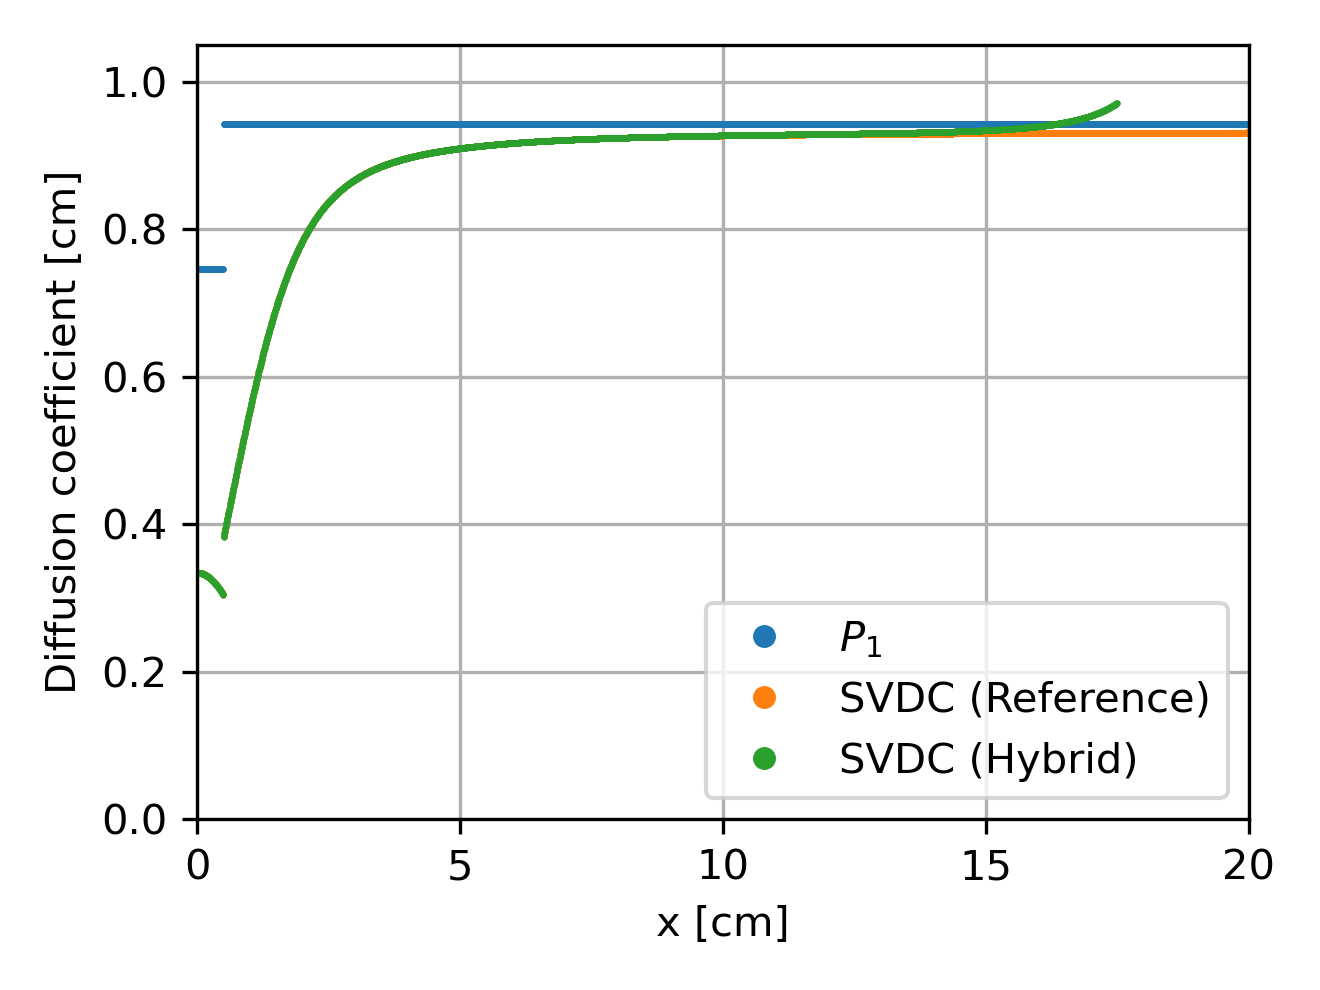
\includegraphics[width=\textwidth]{case-0-group-1-hybrid-diffcoef}
    \caption{Group 1}
    \label{fig:c0g1hd}
  \end{subfigure}
  \hfill
  \begin{subfigure}[b]{.49\textwidth}
    \centering
    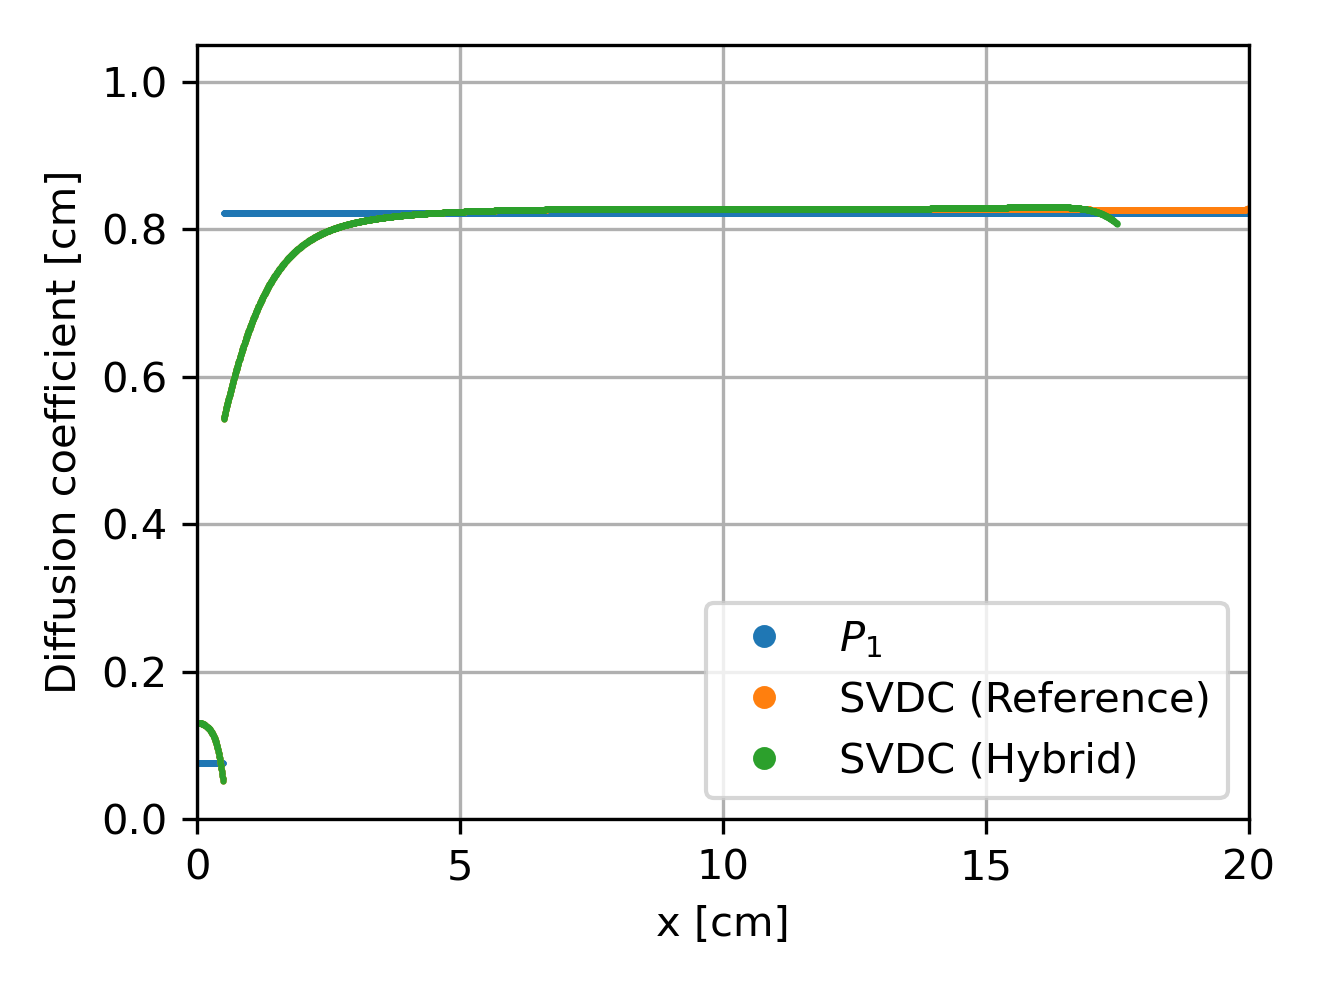
\includegraphics[width=\textwidth]{case-0-group-2-hybrid-diffcoef}
    \caption{Group 2}
    \label{fig:c0g2hd}
  \end{subfigure}
  \caption{$P_1$-based flux-limited diffusion coefficient and \gls{SVDC} spatial distribution for
  Case 0. The \gls{SVDC} distributions were generated from the reference $S_8$ (``SVDC'') and the
  hybrid (``Hybrid'') calculations.}
  \label{fig:c0hd}
\end{figure}

Refer to Figures \ref{fig:c0g1hd} and \ref{fig:c0g2hd} for a qualitative comparison of group 1 and
2 $P_1$-based diffusion coefficients, \glspl{SVDC} derived from the reference $S_8$ calculation as
demonstrated in Section \ref{sec:svdc}, and \glspl{SVDC} derived from the hybrid $S_N$-diffusion
method discussed here. The \glspl{SVDC} from the hybrid method agree well with the reference
\glspl{SVDC} in the control rod region and for most of the fuel-graphite region up to around
$x=15$ cm. Both sets of \glspl{SVDC} approximately coincide with the $P_1$ diffusion coefficient
values within 1\% difference from $x=14.615$ cm and $x=3.390$ cm onwards for group 1 and
group 2, respectively. Accordingly, the buffer region spans from $x=14.615$ cm to $x=17.500$ cm for
group 1 and $x=3.390$ cm to $x=17.500$ cm for group 2, in which the hybrid method defaults to the
$P_1$-based diffusion coefficients. Given that the reference \gls{SVDC} values will generally not
be known in real-world problems, the hybrid method relies on finding the intersection point of the
\gls{SVDC} and $P_1$ diffusion coefficient values to determine the buffer region cutoff point. The
size of $V_1$ will also have to be based on where this intersection point lies.
Another important consideration is the fact that the neutron flux gradient will be discontinuous if
the \gls{SVDC} and $P_1$ diffusion coefficient values are too far apart in magnitude at the buffer
region cutoff point. A flux gradient discontinuity in a homogeneous bulk region is non-physical and
unacceptable. In Section \ref{sec:prelim-results}, I study \gls{SVDC} distribution trends
in more heterogeneous systems and their implications on determining the size of $V_1$ and
the cutoff point.
%
\begin{figure}[htb!]
  \centering
  \begin{subfigure}[b]{.49\textwidth}
    \centering
    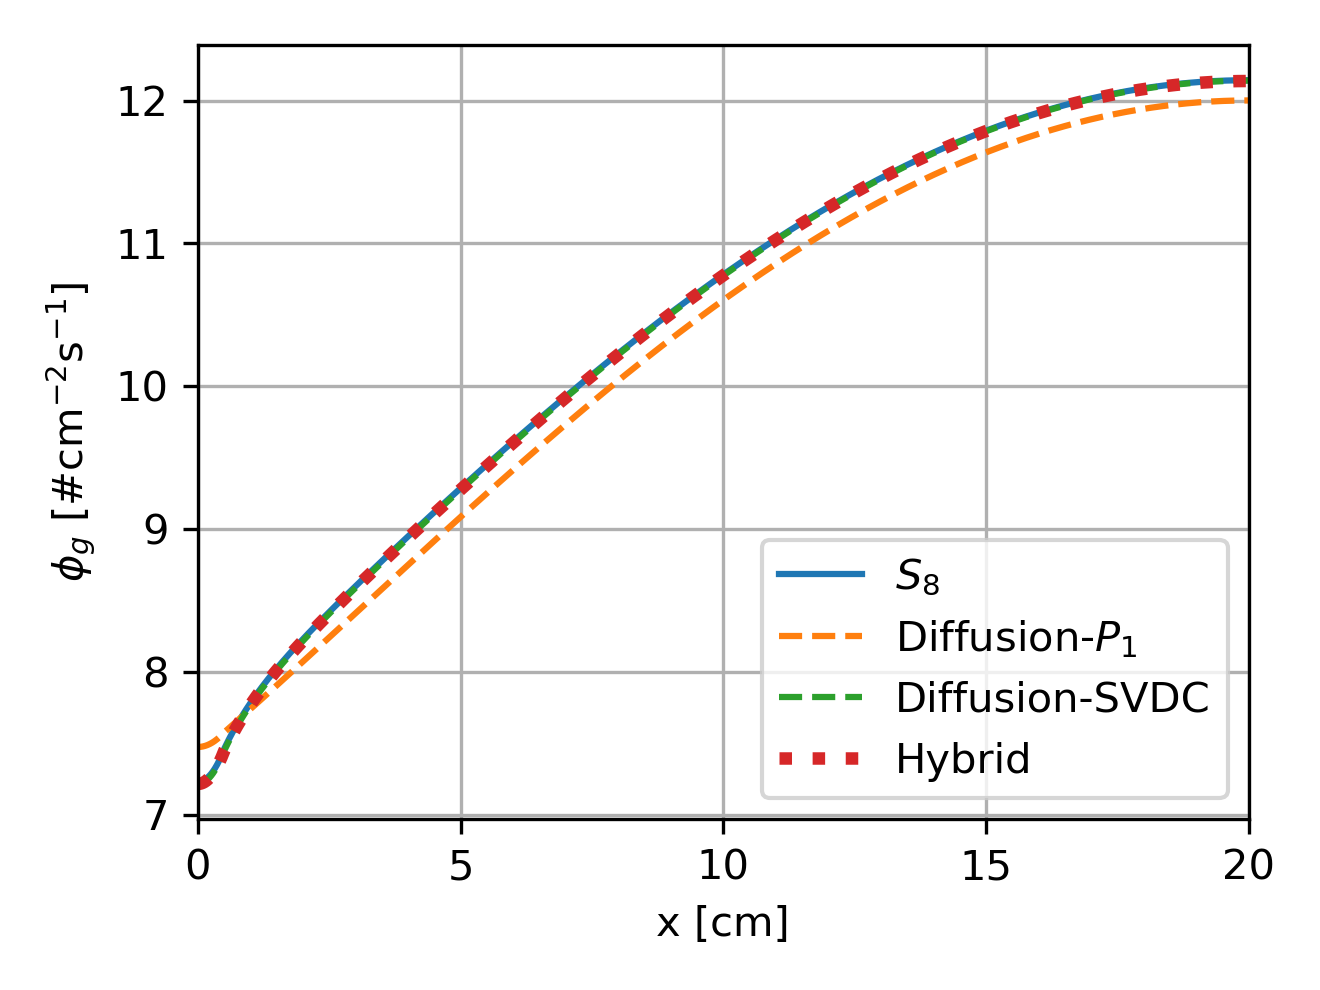
\includegraphics[width=\textwidth]{case-0-group-1-hybrid-flux}
    \caption{Group 1}
    \label{fig:c0g1hf}
  \end{subfigure}
  \hfill
  \begin{subfigure}[b]{.49\textwidth}
    \centering
    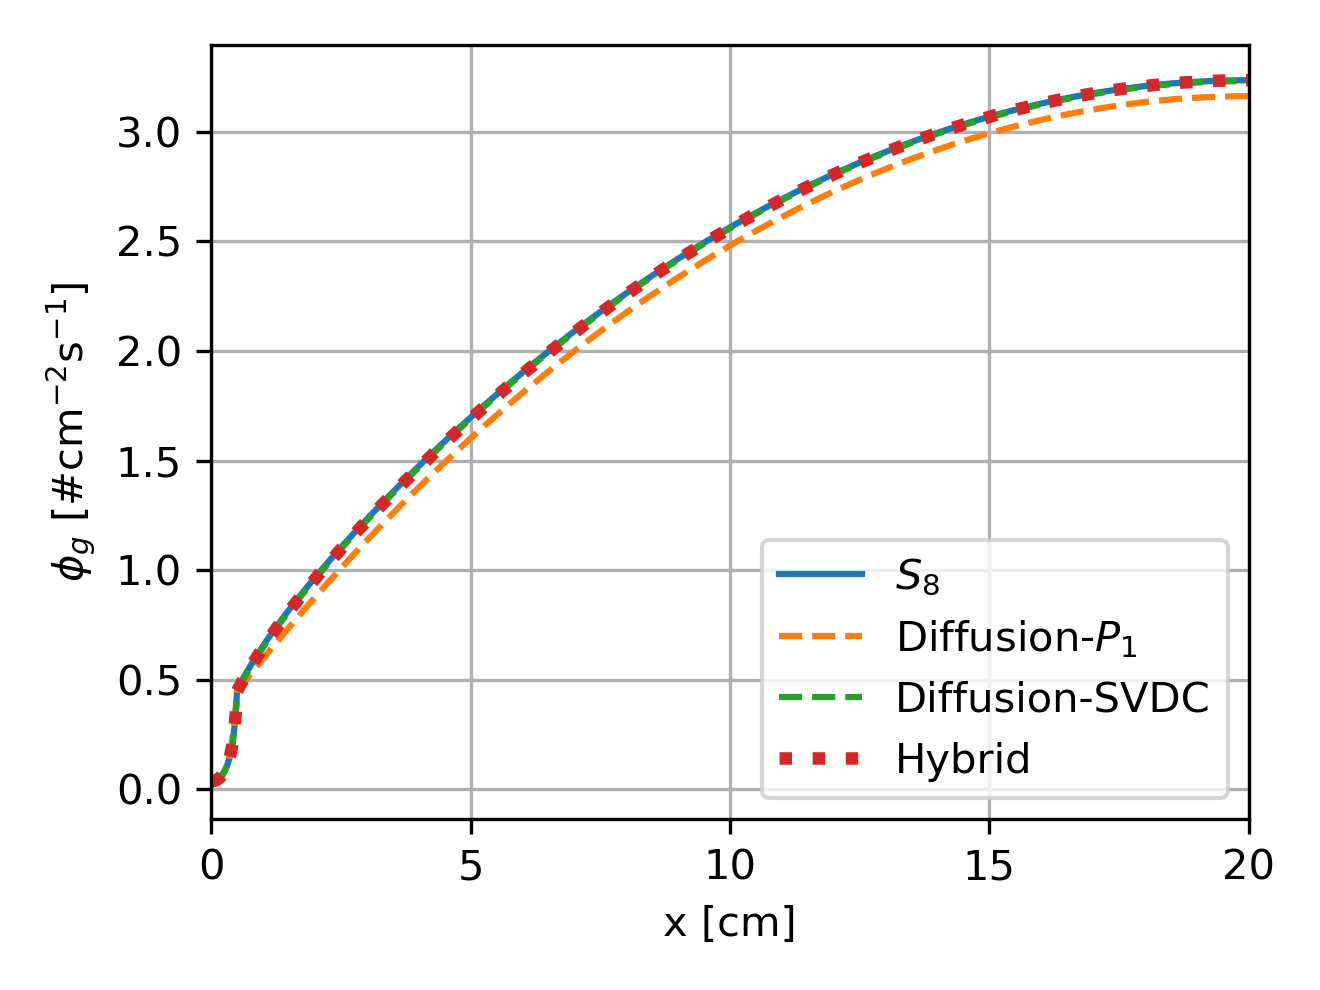
\includegraphics[width=\textwidth]{case-0-group-2-hybrid-flux}
    \caption{Group 2}
    \label{fig:c0g2hf}
  \end{subfigure}
  \caption{Neutron group 1 and 2 flux distributions from the diffusion, $S_8$, reference
  \gls{SVDC}, and hybrid methods for Case 0.}
  \label{fig:c0hf}
  \centering
  \begin{subfigure}[b]{.49\textwidth}
    \centering
    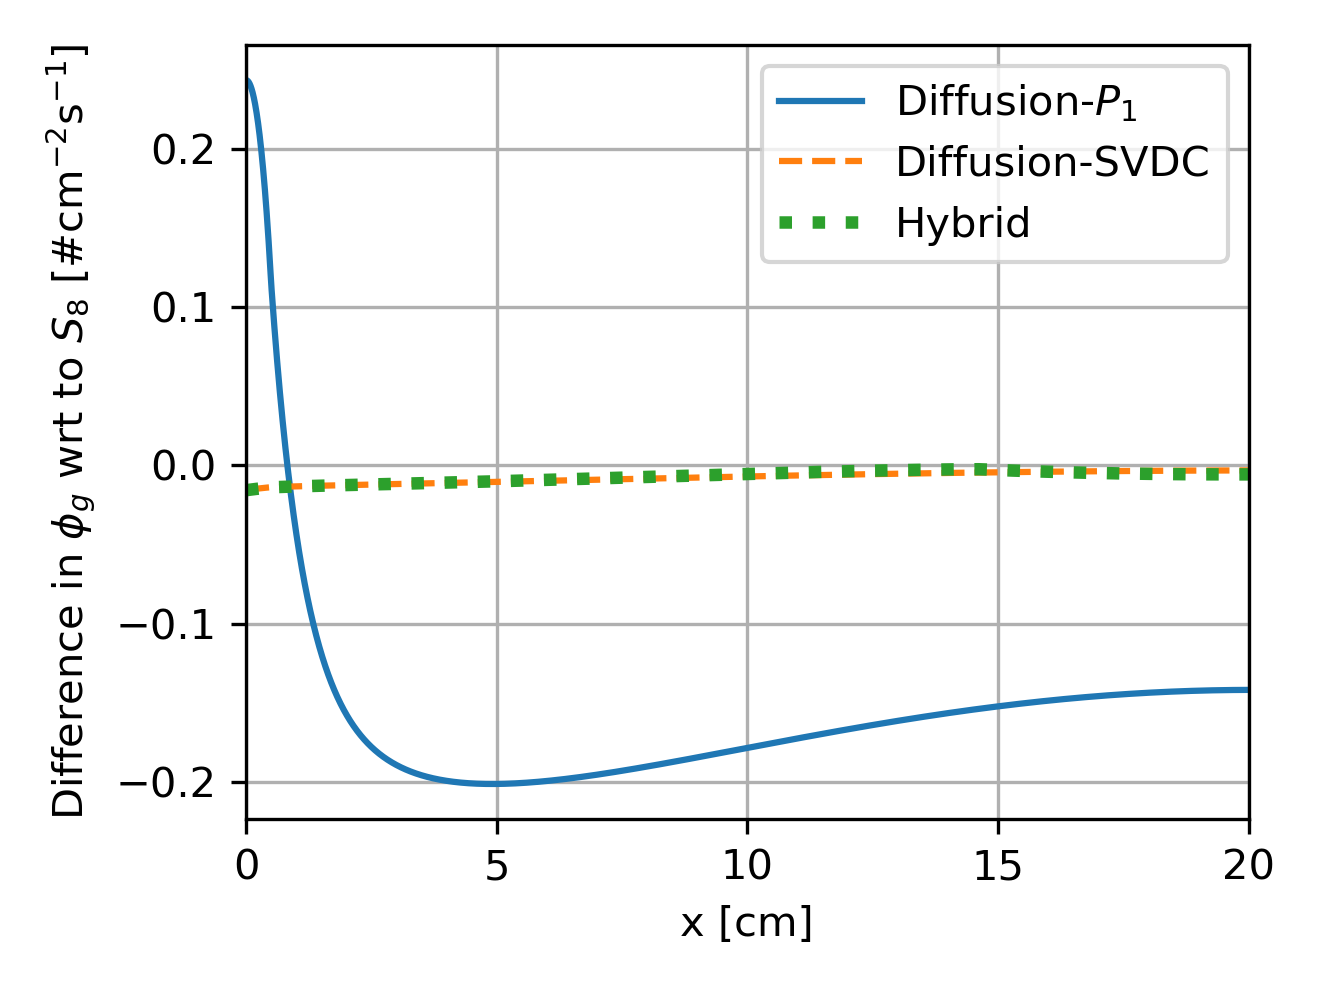
\includegraphics[width=\textwidth]{case-0-group-1-hybrid-flux-diff}
    \caption{Group 1}
    \label{fig:c0g1hfdiff}
  \end{subfigure}
  \hfill
  \begin{subfigure}[b]{.49\textwidth}
    \centering
    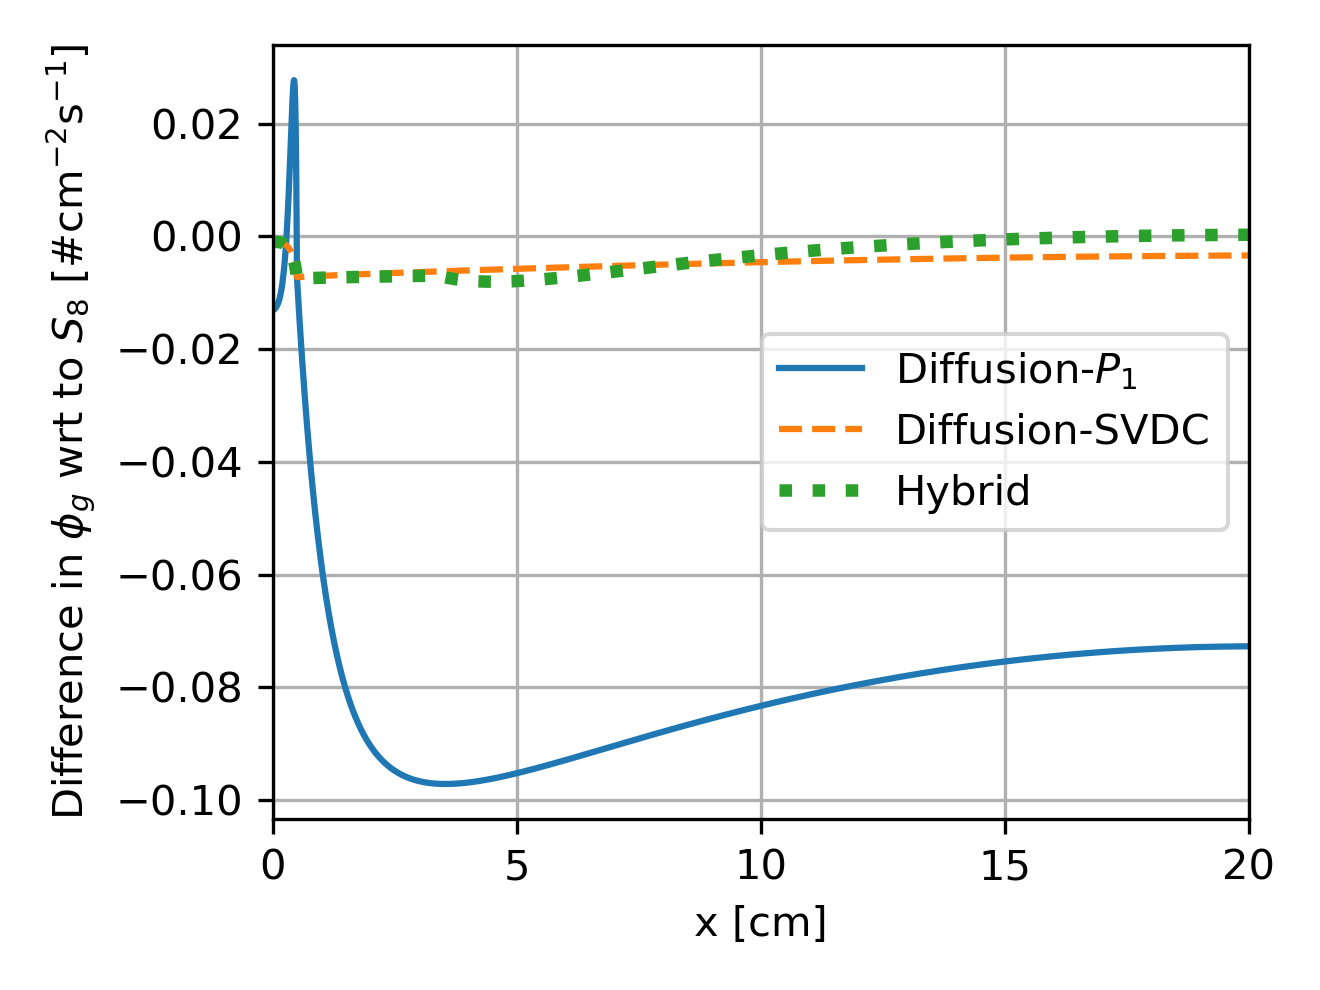
\includegraphics[width=\textwidth]{case-0-group-2-hybrid-flux-diff}
    \caption{Group 2}
    \label{fig:c0g2hfdiff}
  \end{subfigure}
  \caption{Difference in neutron group 1 and 2 flux distributions from the diffusion,
  diffusion-\gls{SVDC}, and hybrid methods with respect to the $S_8$ flux distribution for Case 0.}
  \label{fig:c0hfdiff}
\end{figure}

Figures \ref{fig:c0g1hf} and \ref{fig:c0g2hf} show the group 1 and 2 neutron flux distributions
from the various methods, while Figures \ref{fig:c0g1hfdiff} and \ref{fig:c0g2hfdiff} show the
difference in flux with respect to the $S_8$ flux distribution. As
expected following the diffusion coefficient discussion, the hybrid method flux distribution
matches the $S_8$ and Diffusion-\gls{SVDC} flux distributions well. The $k$ estimate from the
hybrid method is 0.62774, which is only 0.00024 higher than the Diffusion-\gls{SVDC} method, and
0.00038 higher than the $S_8$ method.

In Case 0, $V_1$ covers more than half of $V_0$ due to the control rod region being
the only significant source of influence on the neutron flux distribution in the
otherwise homogeneous system with reflective boundary conditions. I chose Case 0 as a simple test
case to aid in introducing the hybrid $S_N$-diffusion method. In Section \ref{sec:prelim-results},
I present more results with the hybrid method on more complicated geometries containing neutron
reflector, air, and heterogeneous fuel-graphite lattice regions and vacuum boundary conditions. In
these other test cases, the hybrid method yields smaller $V_1$-to-$V_0$ ratios,
reducing computational costs from running $S_N$ calculations over a relatively smaller
region.

\section{Numerical Implementation} \label{sec:implementation}

In Section \ref{sec:theory}, I presented the theoretical basis for the hybrid
$S_N$-diffusion method and demonstrated the method on a simple problem. Now I will discuss
numerical implementation details of group
constant data processing and the neutron diffusion, $S_N$ neutron transport, and hybrid
$S_N$-diffusion solvers. I implemented all numerical solvers and analysis scripts in the Python
programming language. First, I will discuss the material group constant data generation and
postprocessing steps. Next, I present the implementation details of the neutron
diffusion and $S_N$ numerical methods. Lastly, I present how they are coupled to form the hybrid
$S_N$-diffusion method.

\subsection{Group Constant Data Generation}

The group constants required by either or both neutron diffusion and $S_N$ neutron transport
methods are:
%
\begin{itemize}
  \item $\Sigma_{t,g}$: Macroscopic total cross section in group $g$,
  \item $\Sigma_{r,g}$: Macroscopic removal cross section in group $g$,
  \item $\Sigma_s^{g'\rightarrow g}$: Macroscopic group-to-group scattering cross section matrix,
  \item $\Sigma_{s,l}^{g'\rightarrow g}$: $l$-th Legendre moment of the macroscopic
    group-to-group scattering cross section matrix,
  \item $\Sigma_{sp,l}^{g'\rightarrow g}$: $l$-th Legendre moment of the macroscopic
    group-to-group scattering production cross section matrix,
  \item $D_g$: $P_1$-based diffusion coefficient in group $g$,
  \item $\nu\Sigma_{f,g}$: Product of the average number of neutrons produced per fission and the
    macroscopic fission cross section in group $g$,
  \item $\chi_g$: Neutron fission spectrum in group $g$.
\end{itemize}
%
These group constants are generated using OpenMC's multigroup cross section generation capability
\cite{boyd_multigroup_2019} and postprocessed using a Python script into JSON format files.
$\Sigma_{r,g}$ is the only quantity that OpenMC does not directly provide. It is calculated as
%
\begin{align}
  \Sigma_{r,g} =& \sum^G_{g'\neq g}\Sigma_s^{g\rightarrow g'}+\Sigma_{a,g}-\left(\Sigma_{sp}^{g
    \rightarrow g} - \Sigma_s^{g\rightarrow g}\right)
  \shortintertext{where}
      \Sigma_{a,g} =& \mbox{ macroscopic absorption cross section in group $g$,} \nonumber \\
      \Sigma_{sp}^{g\rightarrow g} =& \mbox{ macroscopic scattering production cross section from
      group $g$ to $g$.} \nonumber
\end{align}
%
$\Sigma_{r,g}$ primarily represents the loss of neutrons from group $g$ through outscattering and
absorption. $\Sigma_{sp}^{g\rightarrow g}$ incorporates neutron multiplication effects from neutron
knockout reactions into the scattering cross section. Neutron knockout reactions are commonly
tallied as scattering reactions, and $\Sigma_{r,g}$ is a convenient term to
incorporate neutron knockout effects into the neutron diffusion equations. I ran all test cases for
$S_N$ and hybrid method calculations with up to the 2nd Legendre moments of the scattering
cross sections ($L=2$).

OpenMC uses the $P_1$ flux-limited formulation \cite{pomraning_flux-limited_1984} for calculating
$D_g$ as follows
%
\begin{align}
  D_g =& \frac{1}{3\Sigma_{tr,g}},
  \shortintertext{where}
  \Sigma_{tr,g} =& \frac{\langle\Sigma_{t,g}\phi_g\rangle-\langle\Sigma_{s1,g}\phi_g\rangle}
  {\langle\phi_g\rangle}, \nonumber \\
  \langle\Sigma_{t,g}\phi_g\rangle =& \int_{r\in V}dr \int_{4\pi}d\Omega\int^{E_{g-1}}_{E_g}dE\
  \Sigma_{t,g}(r,E)\Psi(r,E,\Omega), \nonumber \\
  \langle\Sigma_{s1,g}\phi_g\rangle =& \int_{r\in V}dr \int_{4\pi}d\Omega\int^{E_{g-1}}_{E_g}dE
  \int_{4\pi}d\Omega'\int^{\infty}_0dE'\int^1_{-1}d\mu\ \mu\Sigma_s(r,E'\rightarrow E,\Omega'\cdot
  \Omega)\phi(r,E',\Omega'), \nonumber \\
  \langle \phi \rangle =& \int_{r\in V}dr\int_{4\pi}d\Omega\int^{E_{g-1}}_{E_g}dE\ \Psi(r,E,\Omega)
  .\nonumber
\end{align}

\subsection{Neutron Diffusion Method}

On a 1-D uniform spatial grid with $I+1$ mesh points, the neutron scalar flux variables
$\phi_{g,i}$ are defined on the mesh points $x_i$. Theoretically, group constants are volumetric
material properties that should be defined on the cell-centered half-integer mesh points
$x_{i+\sfrac{1}{2}}$. In practice, all material properties except diffusion coefficients are
uniform in each subregion and sampled at $x_i$. To avoid ambiguity concerning diffusion
coefficient sampling, I formulated all test cases such that all material interfaces fall on $x_i$.

Discretizing the multigroup $k$-eigenvalue neutron diffusion equations in Eq. \ref{eq:1d-diff}
and reformulating the scattering term using neutron balance in the control volume bounded by
$x_{i-\sfrac{1}{2}}$ and $x_{i+\sfrac{1}{2}}$ yields
%
\begin{align}
  J_{g,i+\sfrac{1}{2}} - J_{g,i-\sfrac{1}{2}} + \Sigma_{t,g,i} \phi_{g,i} \Delta x = \sum^G_{g'=1}\left[
  \Sigma_{s,i}^{g'\rightarrow g}\phi_{g',i} + \chi_{g,i}\frac{\nu\Sigma_{f,g',i}}{k} \phi_{g',i}
\right]\Delta x. \label{eq:diff-j}
\end{align}
%
Using the diamond difference scheme to replace the $J$ terms with the discretized form of
Fick's first law of diffusion,
%
\begin{align}
  J_{g,i+\sfrac{1}{2}} = -D_{g,i+\sfrac{1}{2}}\frac{d\phi_{g,i+\sfrac{1}{2}}}{dx} =
  -D_{g,i+\sfrac{1}{2}} \frac{\phi_{g,i+1}-\phi_{g,i}}{\Delta x},
\end{align}
%
and rearranging the terms in Eq. \ref{eq:diff-j} yields
%
\begin{align}
  -\frac{D_{g,i-\sfrac{1}{2}}}{\Delta x} \phi_{g,i-1} + &\left[\frac{D_{g,i-\sfrac{1}{2}}+
  D_{g,i+\sfrac{1}{2}}}{\Delta x} + \Delta x\ \Sigma_{r,g,i} \right]\phi_{g,i} -
  \frac{D_{g,i+\sfrac{1}{2}}}{\Delta x}\phi_{g,i+1} -\Delta x\sum^G_{g'\neq g}
  \Sigma_{s,i}^{g'\rightarrow g}\phi_{g',i} \nonumber \\
  =& \Delta x\sum^G_{g'=1}
  \chi_{g,i} \frac{\nu\Sigma_{f,g',i}}{k} \phi_{g',i}, \label{eq:diff-fd}
  \shortintertext{where}
  \Sigma_{r,g} =& \Sigma_{t,g} - \Sigma_s^{g\rightarrow g} \nonumber \\
  =& \mbox{ macroscopic removal cross section for neutron group }g. \nonumber
\end{align}
%
The diamond difference scheme is 2nd-order accurate, and this form is
equivalent to applying 2nd-order finite differencing to the original neutron diffusion equation in
Eq. \ref{eq:1d-diff} with diamond differencing for the cell-centered group constants.
The fixed neutron source $S_g$ is ignored here since the test cases are all neutron-multiplying
systems with no fixed source.

I implemented two types of boundary conditions: vacuum and reflective boundary conditions. The
\textbf{vacuum boundary conditions} are imposed by setting the incoming flux in the $P_1$
approximation to zero and applying 2nd-order finite differencing as follows:
%
\begin{align}
  \mbox{Left boundary: } \frac{\phi_{g,0}}{4}-\frac{D_{g,\sfrac{1}{2}}}{2}
  \frac{\left(-\phi_{g,2}+4\phi_{g,1}-3\phi_{g,0}\right)}{2\Delta x} =& 0 \\
  \mbox{Right boundary: } \frac{\phi_{g,I}}{4}+\frac{D_{g,I-\sfrac{1}{2}}}{2}
  \frac{\left(\phi_{g,I-2}-4\phi_{g,I-1}+3\phi_{g,I}\right)}{2\Delta x} =& 0.
\end{align}
%
The \textbf{reflective boundary conditions} are imposed by setting the flux gradient to zero and
applying 2nd-order finite differencing as follows:
%
\begin{align}
  \mbox{Left boundary: } \frac{-3\phi_{g,0}+4\phi_{g,1}-\phi_{g,2}}{2\Delta x} =& 0 \\
  \mbox{Right boundary: } \frac{3\phi_{g,I}-4\phi_{g,I-1}+\phi_{g,I-2}}{2\Delta x} =& 0
\end{align}
%
At material interfaces, the continuity condition requires that the net neutron current on either
side of the interface be equal as follows:
%
\begin{align}
  -\frac{3D_{g,i-\sfrac{1}{2}} - D_{g,i-\sfrac{3}{2}} }{2}
  \frac{\phi_{g,i-2}-4\phi_{g,i-1}+3\phi_{g,i}}{2\Delta x} =&
  -\frac{3D_{g,i+\sfrac{1}{2}} - D_{g,i+\sfrac{3}{2}} }{2}
  \frac{-3\phi_{g,i}+4\phi_{g,i+1}-\phi_{g,i}}{2\Delta x} \label{eq:itf-bc}
\end{align}
%
for a material interface at $x_i$.

Altogether, they form a system of equations of the form $\bm{A\overline{\phi}}=\bm{\frac{1}{k}
B\overline{\phi}}$, where $\bm{\overline{\phi}}$ is a flattened vector representation of
$\phi_{g,i}$, and $\bm{A}$ and $\bm{B}$ are matrices of the coefficients of $\phi_{g,i}$ as given
by Eqs. \ref{eq:diff-fd} to \ref{eq:itf-bc}. I implemented the inverse power method to find $k$ and
$\overline{\phi}$. The inverse power method algorithm is as follows
%
\begin{align}
  \shortintertext{1. Initialize $k^0$ and $\bm{\overline{\phi}}^0$}
  \shortintertext{2. Update $\bm{\overline{\phi}}$ and $k$}
  \bm{\overline{\phi}}^m =& \frac{1}{k^{m-1}}\bm{A}^{-1}\bm{B\overline{\phi}}^{m-1} \\
  k^m =& k^{m-1}\frac{|\bm{B\overline{\phi}}^m|}{|\bm{B\overline{\phi}}^{m-1}|}
  \shortintertext{3. Check whether convergence is reached}
  \epsilon_\phi =
  \frac{|\bm{\overline{\phi}}^m-\bm{\overline{\phi}}^{m-1}|}{|\bm{\overline{\phi}}^m|} <& \
  tol_{\bm{\overline{\phi}}} \\
  \epsilon_k =
  \frac{|k^m-k^{m-1}|}{|k^m|} <& \ tol_k
  \shortintertext{4. Return to Step 2 if either expression is false, otherwise exit.} \nonumber
\end{align}
%
$k^m$ and $\overline{\phi}^m$ denote estimates of $k$ and $\overline{\phi}$ after the $m$-th
iteration. Matrix $\bm{A}$ is a primarily tridiagonal matrix with at most $G-1$ off-diagonal terms
from the fourth term in Eq. \ref{eq:diff-fd}. Thus, $\bm{A}$ is initialized as a sparse matrix to
take advantage of the computationally efficient sparse matrix solver functions from the
\texttt{sparse} class of the \texttt{SciPy} \cite{virtanen_scipy_2020} Python library for
scientific and technical computing. Matrix $\bm{B}$
is never initialized explicitly as a matrix. Instead, the vector $\bm{b}=\bm{B\overline{\phi}}$ is
updated directly in every iteration. In this system of equations, $|\bm{b}|$ corresponds to the
total number of fission neutrons produced in the system for a given $\bm{\overline{\phi}}$. This
quantity is calculated using the \texttt{trapezoid} numerical integration function from
\texttt{SciPy} to estimate the integral value of the source term, $\nu\Sigma_{g,f}\phi_{g}$, in $x$
from the discrete flux values in $\bm{x}$. Finally, the final $\phi_{g,i}$ is normalized by a
factor of $|\bm{b}|/k$ (no. of source neutrons) to obtain the neutron scalar flux per source
neutron.

\subsection{$S_N$ Neutron Transport Method}

For the 1-D $S_N$ neutron transport method on the same uniform spatial grid with $I+1$ mesh points,
the neutron angular flux variables $\Psi_{g,i,n}=\Psi_g(x_i,\mu_n)$ are defined on the mesh points
$x_i$ while neutron scalar flux variables $\phi_{g,i\pm\sfrac{1}{2}}=\phi_g(x_{i\pm\sfrac{1}{2}})$
are defined on the half-integer mesh points $x_{i\pm\sfrac{1}{2}}$. All group constants are sampled
at $x_{i\pm\sfrac{1}{2}}$.

The $S_N$ equations are solved using the transport sweep method in which the algorithm ``sweeps''
through the spatial grid and sequentially updates $\Psi_{g,i,n}$. The algorithm sweep
direction follows the direction of neutron travel, i.e. it sweeps in the positive direction for
$\Psi_{g,i,n}$ with $\mu_n>0$ and vice versa. Doing otherwise is unphysical and causes numerical
instabilities.

Discretizing the multigroup $S_N$ neutron transport equations in Eq. \ref{eq:1d-sn} about
$x_{i+\sfrac{1}{2}}$ yields
%
\begin{align}
  \mu_n\frac{\Psi_{g,i+1,n}-\Psi_{g,i,n}}{x_{i+1}-x_i} + \Sigma_{t,g,i+\sfrac{1}{2}}
  \Psi_{g,i+\sfrac{1}{2},n} = q_{g,i+\sfrac{1}{2},n}
\end{align}
%
where $q_{g,i+\sfrac{1}{2},n}$ represents the combined scattering and fission neutron source term.
After expressing $\Psi_{g,i+\sfrac{1}{2}}$ as the average of $\Psi_{g,i+1,n}$ and $\Psi_{g,i,n}$
in the diamond difference scheme and rearranging the terms, we obtain
%
\begin{align}
  \Psi_{g,i+1,n} =& \frac{1-\Sigma_{t,g}\Delta x/2\mu_n}{1+
    \Sigma_{t,g}\Delta x/2\mu_n}\Psi_{g,i,n} +
    q\frac{\Delta x}{\mu_n\left(1+\Sigma_{t,g}\Delta x/2\mu_n\right)} \label{eq:sweep-right} &&
    (\mbox{for } \mu_n > 0)
\shortintertext{and}
  \Psi_{g,i,n} =& \frac{1+\Sigma_{t,g}\Delta x/2\mu_n}{1-
    \Sigma_{t,g}\Delta x/2\mu_n}\Psi_{g,i+1,n} -
    q\frac{\Delta x}{\mu_n\left(1-\Sigma_{t,g}\Delta x/2\mu_n\right)}. \label{eq:sweep-left} &&
    (\mbox{for } \mu_n < 0)
\end{align}
%
The remaining $i+\sfrac{1}{2}$ indexes on the group constants are dropped to reduce visual clutter.
These expressions are used to update $\Psi_{g,i,n}$ in the forward and backward transport sweeps.

The discretized scattering and fission terms in $q_{g,i+\sfrac{1}{2},n}$ are given as
%
\begin{align}
  q_{g,i+\sfrac{1}{2},n} =& \sum^G_{g'=1}\sum^L_{l=0}\frac{\left(2l+1\right)}
  {2}\Sigma_{s,l}^{g'\rightarrow g}P_l(\mu_n)\phi_{l,g',i+\sfrac{1}{2}} \nonumber \\
  &+\frac{\chi_g}{2}\sum^G_{g'=1}\frac{\nu\Sigma_{f,g'}}{k}\phi_{0,g',i+\sfrac{1}{2}}
  \label{eq:sn-q}
  \shortintertext{where}
  \phi_{l,g',i+\sfrac{1}{2}} =& \sum^N_{n'=1}w_{n'}P_l(\mu_{n'})\frac{\Psi_{g',i,n'}+
  \Psi_{g',i+1,n'}}{2}. \label{eq:phi-l}
\end{align}
%
$\phi_{l,g,i}$ are $l$-th Legendre expansions of the neutron flux evaluated using Gauss-Legendre
quadrature over $\mu_{n'}=[-1,1]$. $\phi_{0,g,i}$ and $\phi_{1,g,i}$ also correspond to the neutron
scalar flux $\phi_{g,i}$ and net current $J_{g,i}$, respectively.

For vacuum boundary conditions, $\Psi_{g,0,n}$ is zero for all positive $\mu_n$ while
$\Psi_{g,I,n}$ is zero for all negative $\mu_n$ as follows
%
\begin{align}
  \mbox{Left boundary: } \Psi_{g,0,n} =& 0 && (\mbox{for } \mu_n > 0) \\
  \mbox{Right boundary: } \Psi_{g,I,n} =& 0 && (\mbox{for } \mu_n < 0)
\end{align}
%
Reflective boundary conditions are imposed by equating the incoming angular flux to the
outgoing angular flux in the opposite direction as follows
%
\begin{align}
  \mbox{Left boundary: } \Psi_{g,0,n} =& \Psi_{g,0,n'} && (\mbox{for } \mu_n > 0, \mu_n =
  -\mu_{n'}) \\
  \mbox{Right boundary: } \Psi_{g,I,n} =& \Psi_{g,I,n'} && (\mbox{for } \mu_n < 0, \mu_n =
  -\mu_{n'})
\end{align}

The power iteration algorithm for the $S_N$ method is similar to the inverse power method algorithm
applied in the neutron diffusion method. The transport sweep step replaces the matrix-solving step
for updating $\overline{\phi}$.
%
\begin{align}
  \shortintertext{1. Initialize $k^0$, $\phi_{l,g,i+\sfrac{1}{2}}^0$, and $q^0$}
  \shortintertext{2. Apply transport sweeps to solve for $\Psi^m$ using Eqs. \ref{eq:sweep-right},
  \ref{eq:sweep-left}, and \ref{eq:sn-q}}
  \shortintertext{3. Update $\phi^m$ and $k^m$ using Eqs. \ref{eq:phi-l} and \ref{eq:sn-k}}
  k^m =& k^{m-1}\frac{\sum^I_{i=0}\sum^G_{g=1}\nu\Sigma_{f,g}\phi^m_{g,i+\sfrac{1}{2}}}
  {\sum^I_{i=0}\sum^G_{g=1}\nu\Sigma_{f,g}\phi^{m-1}_{g,i+\sfrac{1}{2}}} \label{eq:sn-k}
  \shortintertext{4. Check whether convergence is reached}
  \epsilon_\phi =
  \frac{|\bm{\overline{\phi}}^m-\bm{\overline{\phi}}^{m-1}|}{|\bm{\overline{\phi}}^m|} <& \
  tol_{\bm{\overline{\phi}}} \\
  \epsilon_k =
  \frac{|k^m-k^{m-1}|}{|k^m|} <& \ tol_k
  \shortintertext{5. Return to Step 2 if either expression is false, otherwise exit.} \nonumber
\end{align}

The transport sweep and $\phi^m$-update algorithms are parallelized using the \texttt{joblib}
parallel computing Python library \cite{noauthor_joblib_nodate} across all available CPU threads.
The total computational work is subdivided into several smaller tasks classified by unique pairs
of $g$ and $n$ values; each thread computes all $\Psi^m$ or $\phi^m$ values on the mesh for a given
pair of indexes $g$ and $n$.

\subsection{Hybrid $S_N$-Diffusion Method}

Without loss of generality, consider a 1-D system symmetric about the left boundary at $x_0=0$ cm.
In this case, as with Case 0, the control rod region is the left-most region, followed by other
regions. The $S_N$ subproblem domain $V_1$, containing the control rod and some region beyond it,
is bounded by $x_0$ and $x_j$ for some $x_j$
located several mean free paths to the right of the control rod region as governed by the relevant
discussion in Section \ref{sec:hybrid-method}.

Excluding the initial neutron diffusion calculation to initialize $k^0$ and $\phi^0$, each outer
iteration in the hybrid method consists of one $S_N$ neutron transport calculation and one neutron
diffusion calculation. The $\phi$ estimates from these $S_N$ transport and neutron diffusion
calculations are labeled as $\phi^{m+\sfrac{1}{2}}$ and $\phi^{m+1}$ during the
$(m+1)$-th outer iteration. $\phi^{m+\sfrac{1}{2}}$ spans $V_1$ while $\phi^{m+1}$ spans
the entire domain $V_0$.

For the $S_N$ subproblem boundary conditions, we discretize Eqs. \ref{eq:p1-j} and
\ref{eq:sn-psi-j} as follows
%
\begin{align}
  \Psi_{g,j,n} =& \frac{J_{g,-}(x_j)}{\sum^{N/2}_{n'=1}w_{n'}\mu_{n'}} \nonumber \\
  =& \frac{\frac{\phi_g(x_j)}{4}+
  \frac{D_g(x_{j-\sfrac{1}{2}})}{2}\frac{d\phi_g(x_j)}{dx}}{\sum^{N/2}_{n'=1}w_{n'}\mu_{n'}}
  \nonumber \\
  =& \frac{\frac{\phi_{g,j}}{4}+
  \frac{D_{g,j-\sfrac{1}{2}}}{2}\frac{\phi_{g,j}-\phi_{g,j-1}}{\Delta x}}
    {\sum^{N/2}_{n'=1}w_{n'}\mu_{n'}} && (\mu_n < 0) \label{eq:sn-bc}
\end{align}
%
where $D_g$ is the $P_1$-based diffusion coefficient value.

The \gls{SVDC} formulation in Eq. \ref{eq:svdc} is discretized using the diamond difference scheme
as follows
%
\begin{align}
  D^s_{g,i+\sfrac{1}{2}} =& -\frac{J^{tr}_{g,i+1}+J^{tr}_{g,i}}{2} \left(
  \frac{\phi^{tr}_{g,i+1}-\phi^{tr}_{g,i}}{\Delta x} \right)^{-1} = -\frac{\Delta x}{2}
  \frac{J^{tr}_{g,i+1}+J^{tr}_{g,i}}{\phi^{tr}_{g,i+1}-\phi^{tr}_{g,i}}. \label{eq:svdc-num}
\end{align}
%
%From Eq. \ref{eq:svdc-num}, we note that numerical instabilities may occur near flux peaks where
%the flux gradient and thus the denominator of Eq. \ref{eq:svdc-num} approach zero. On the other
%hand, this observation also implies that diffusion coefficient values have negligible influence on
%the flux solution near flux peaks due to the small flux gradient values. Therefore, we can avoid
%numerical instabilities by applying the following logic after calculating $D^s_g$: If the ratio of
%$|\frac{d\phi_g}{dx}|$ to $|\phi_g|$ is sufficiently small and $|D^s_g-D_g| > D_g$, the hybrid
%method defaults to using $D_g$ instead of $|D^s_g-D_g|$. The first conditional statement locates
%regions of relatively flat flux, and of these regions, the second conditional statement excludes
%regions which naturally experience flat flux such as air-filled regions. In all test cases,
%applying the first conditional as $|\frac{1}{\phi_g}\frac{d\phi_g}{dx}|<5\times 10^{-2}$ was
%sufficient for this task.

The hybrid $S_N$-diffusion algorithm is as follows
%
\begin{align}
  \shortintertext{1. Initialize $k^0$ and $\phi^0$ with an initial neutron diffusion calculation on
  $V_0$}
  \shortintertext{2. Generate estimates for $\Psi_{g,j,n}$ at $x_j$ for the $S_N$ transport
  calculation boundary conditions using Eq. \ref{eq:sn-bc}}
  \shortintertext{3. Calculate $\phi^{m+\sfrac{1}{2}}$ with the $S_N$ transport sub-solver on
  $V_1$}
  \shortintertext{4. Generate \glspl{SVDC} with $\phi^{m+\sfrac{1}{2}}$ and $J^{m+\sfrac{1}{2}}$
  using Eq. \ref{eq:svdc-num}}
  \shortintertext{5. Calculate $\phi^{m+1}$ with the newly generated \glspl{SVDC} and the neutron
  diffusion solver on $V_0$}
  \shortintertext{6. Check whether convergence is reached}
  \frac{|\bm{\overline{\phi}}^m-\bm{\overline{\phi}}^{m-1}|}{|\bm{\overline{\phi}}^m|} <& \
  tol_{\bm{\overline{\phi}}} \\
  \frac{|k^m-k^{m-1}|}{|k^m|} <& \ tol_k
  \shortintertext{7. Return to Step 2 if either expression is false, otherwise exit.} \nonumber
\end{align}
%
Generally, the convergence tolerance values for the outer hybrid method iteration must be smaller
than the tolerance values for the neutron diffusion and $S_N$ transport inner iterations. Using
$\phi^m$ from the neutron diffusion calculation as initial conditions for the $S_N$ transport
calculation in the $(m+1)$-th iteration helps to reduce the number of transport
sweeps required significantly.

The $S_N$ sub-solver only covers $V_1$, so it does not calculate an independent $k$
estimate. Instead, the $k^m$ from the neutron diffusion calculation scales the fission neutron
source term in the $S_N$ sub-solver.

\section{Description of 1-D Test Cases} \label{sec:test-case}

I designed ten 1-D test cases with increasing complexity to test the performance of the hybrid
$S_N$-diffusion method in response to various geometrical features. The last two cases resemble the
reference \gls{MSRE} design \cite{robertson_msre_1965}, which has centrally located control rods
and air-filled rod guide tubes. Figure \ref{fig:case-geom} shows the geometries of Cases 0 to
5b. All geometries have reflective boundary conditions at $x=0$ cm to reduce computational costs by
creating half-core or repeating unit cell models. Cases 1a, 2a, 3a, and 4a are repeating unit
cell models with reflecting boundaries on the right-side boundaries. Cases 1b, 2b, 3b, 4b, 5a, and
5b are half-core models with vacuum boundaries on the right-side boundaries.

Starting with an infinite, homogeneous region in Case 1a, I systematically added geometric
complexities to each successive test case to identify how each feature impacts the neutronics
results. Case 1b introduces a reflector region and vacuum boundary conditions relative to Case 1a.
Cases 2a and 2b introduce a control rod region between $x=0$ cm and $x=0.5$ cm relative to Cases 1a
and 1b. Cases 3a and 3b introduce a 0.5 cm-thick air gap between the control rod and the
fuel-graphite mixture regions relative to Cases 2a and 2b. For Cases 4a and 4b, I replaced the
homogeneous fuel-graphite mixture in Cases 1a and 2b with explicit fuel-graphite lattices, as shown
in Figure \ref{fig:case-geom}. Case 5a introduces an air gap between the control rod and the
fuel-graphite lattice regions. Lastly, Case 5b replaces the control rod region with an extended
air gap region to provide a base case for the control rod worth calculations relative to Case 5a.

The cases that do not contain control rod regions (1a, 1b, 4a, 4b, and 5b) serve as reference cases
to quantify other sources of discrepancies in the neutron diffusion solution (e.g., geometrical
heterogeneities, vacuum boundary condition approximation for neutron diffusion) and highlight how
much the neutron diffusion method underperforms when the problem includes control rod regions.

\begin{figure}[htb!]
  \centering
  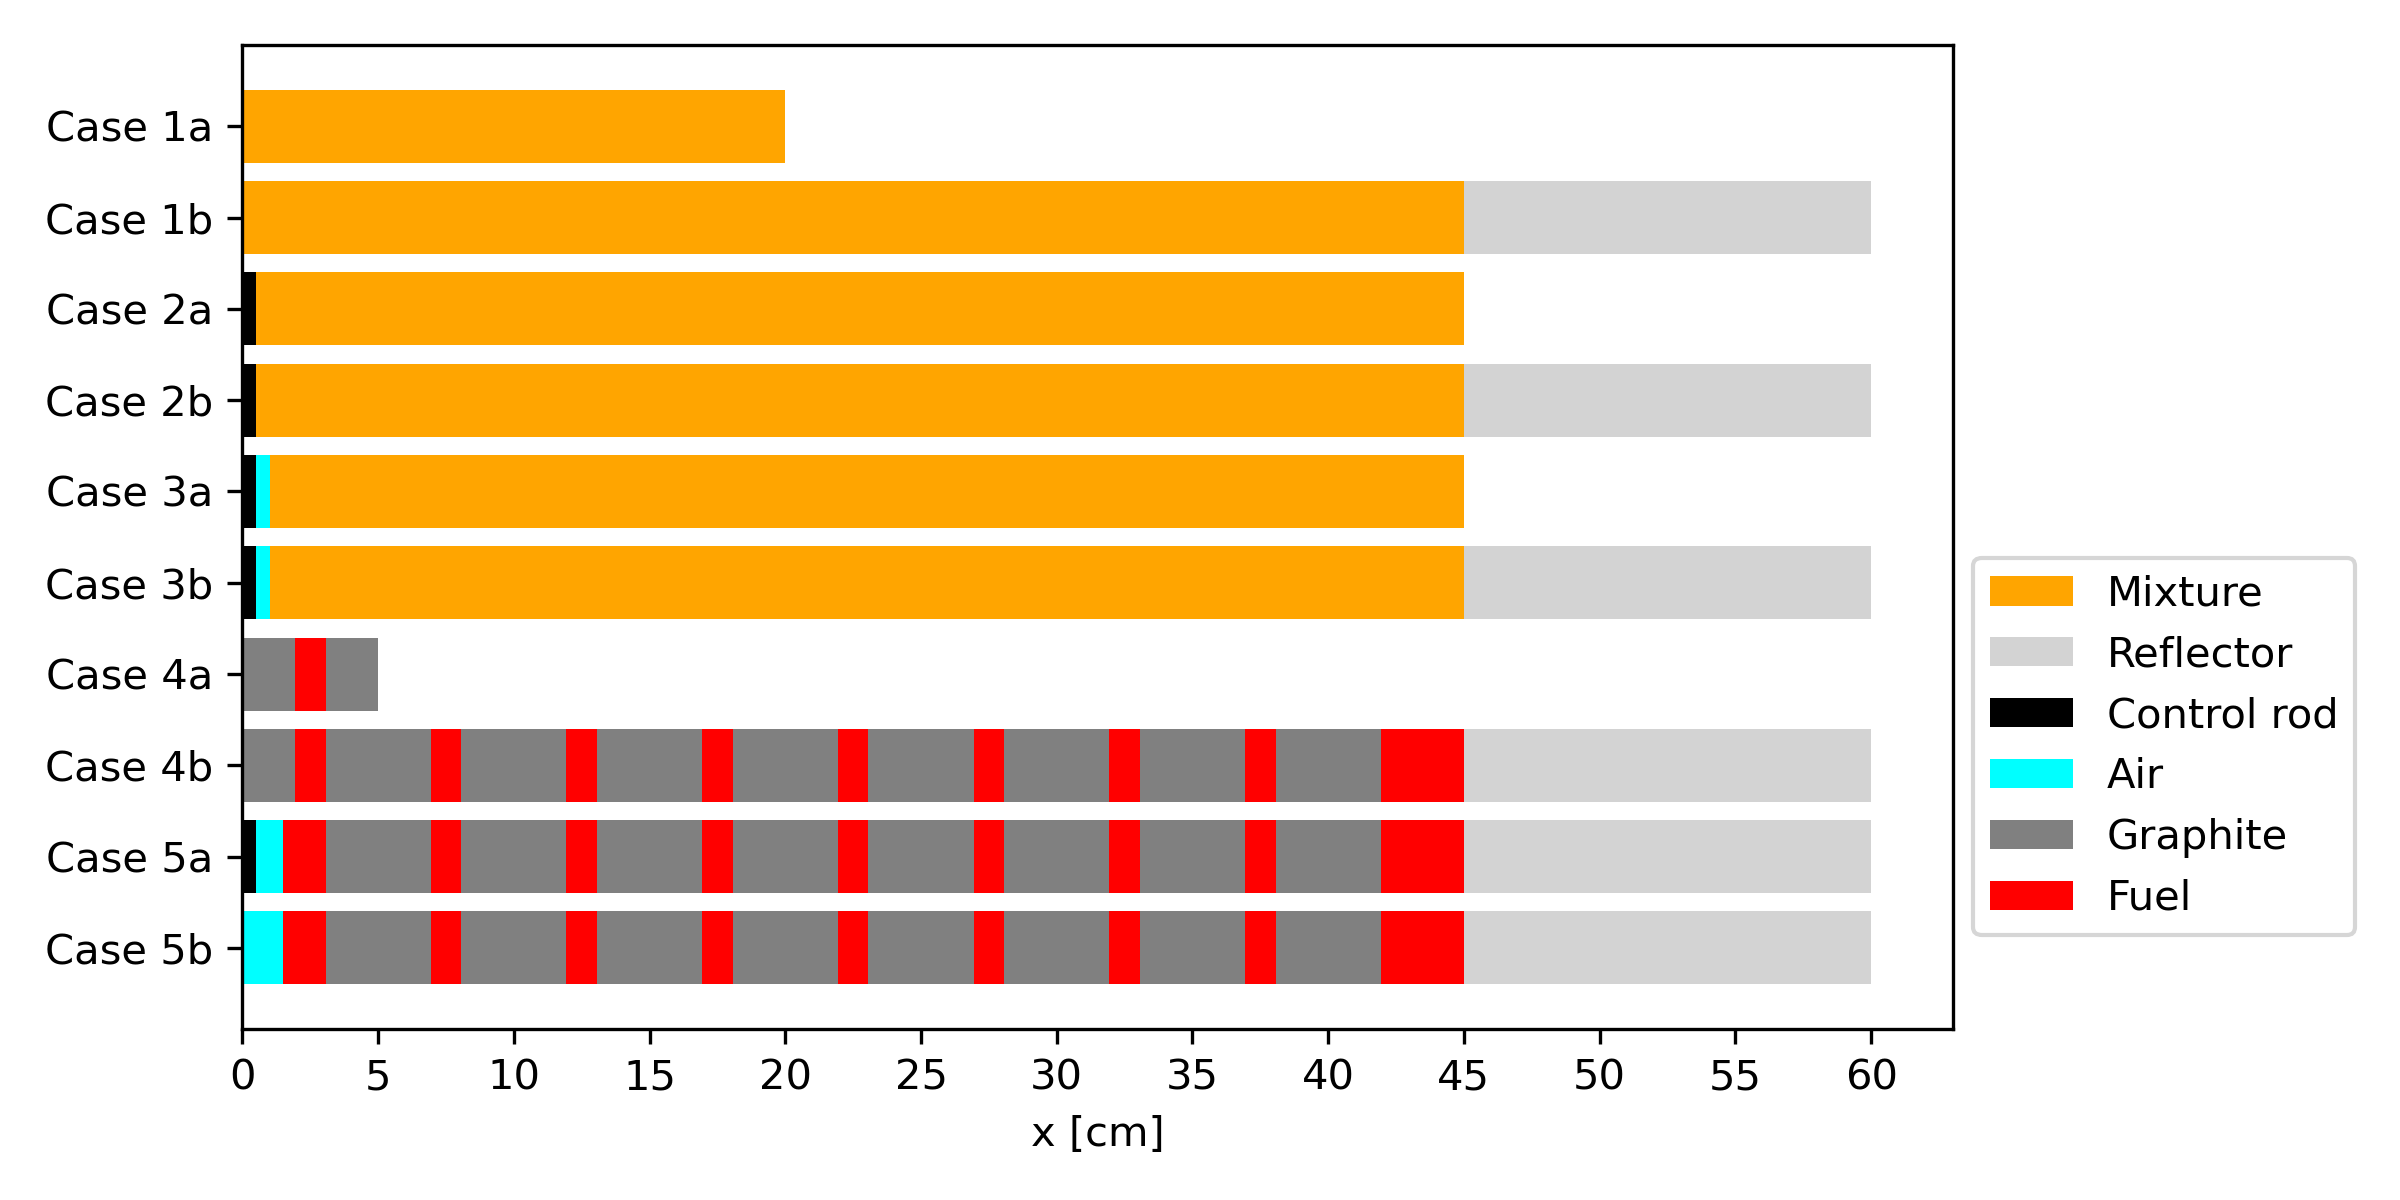
\includegraphics[width=\columnwidth]{case-geometry}
  \caption{Geometries of the 1-D test cases. The material labeled ``mixture'' represents a
    homogeneous mixture of fuel and graphite at a ratio of 22.5\%-77.5\% by volume. All geometries
    have reflective boundary conditions on the boundary at $x=0$ cm. The right-side boundaries are
    reflective for Cases 1a, 2a, 3a, and 4a, and vacuum for Cases 1b, 2b, 3b, 4b, 5a, and 5b.}
  \label{fig:case-geom}
\end{figure}
%
\begin{figure}[htb!]
  \centering
  \begin{subfigure}[t]{.49\textwidth}
    \centering
    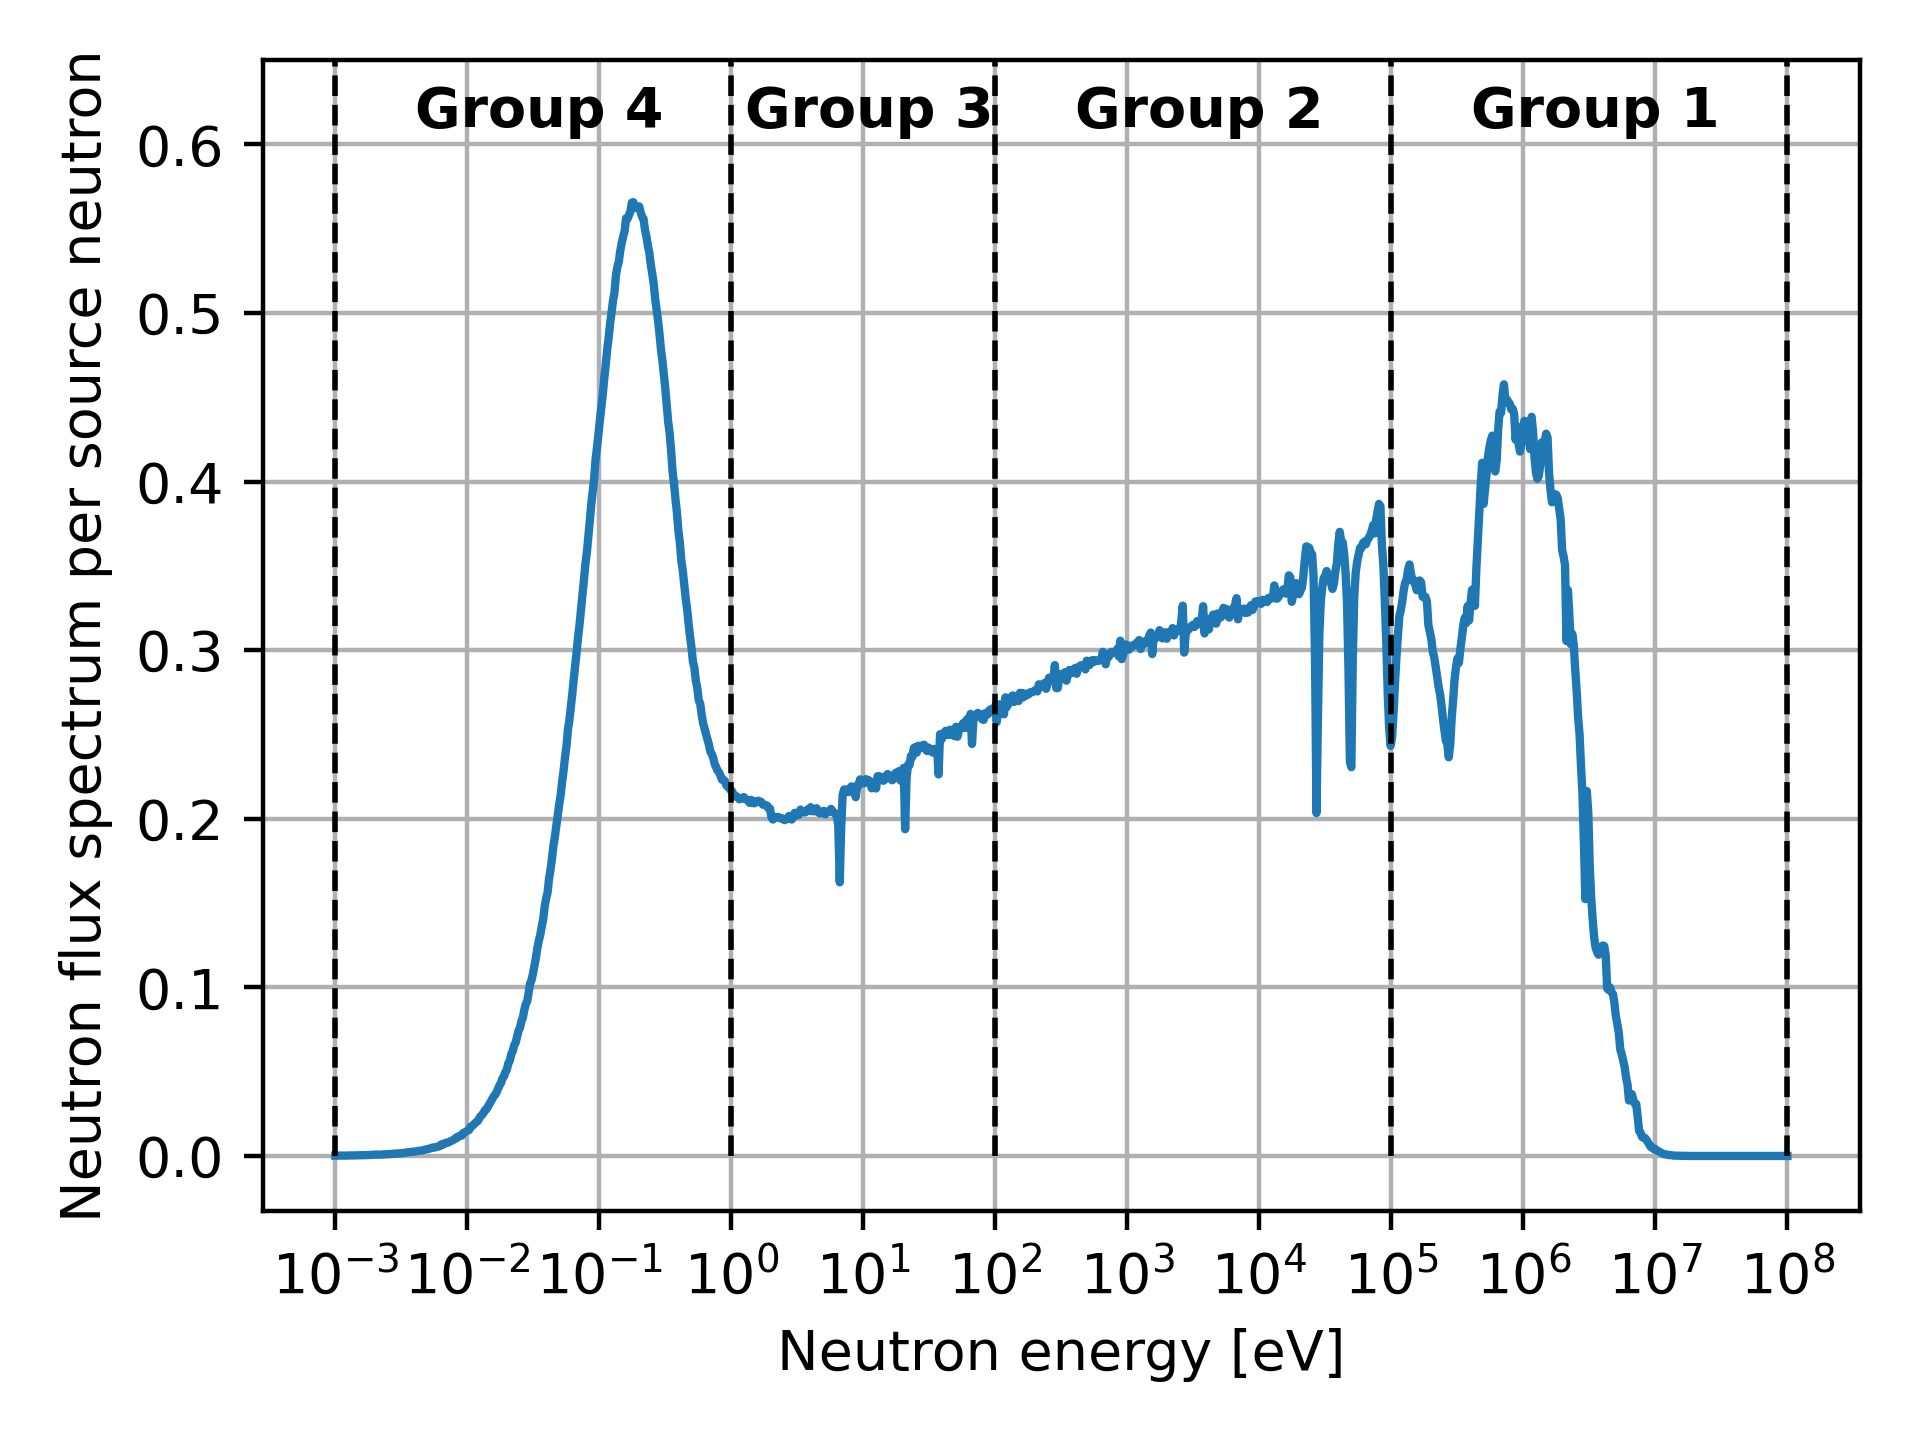
\includegraphics[width=\textwidth]{spectrum}
    \caption{Neutron flux energy spectrum per source neutron}
    \label{fig:spectrum}
  \end{subfigure}
  \hfill
  \begin{subfigure}[t]{.49\textwidth}
    \centering
    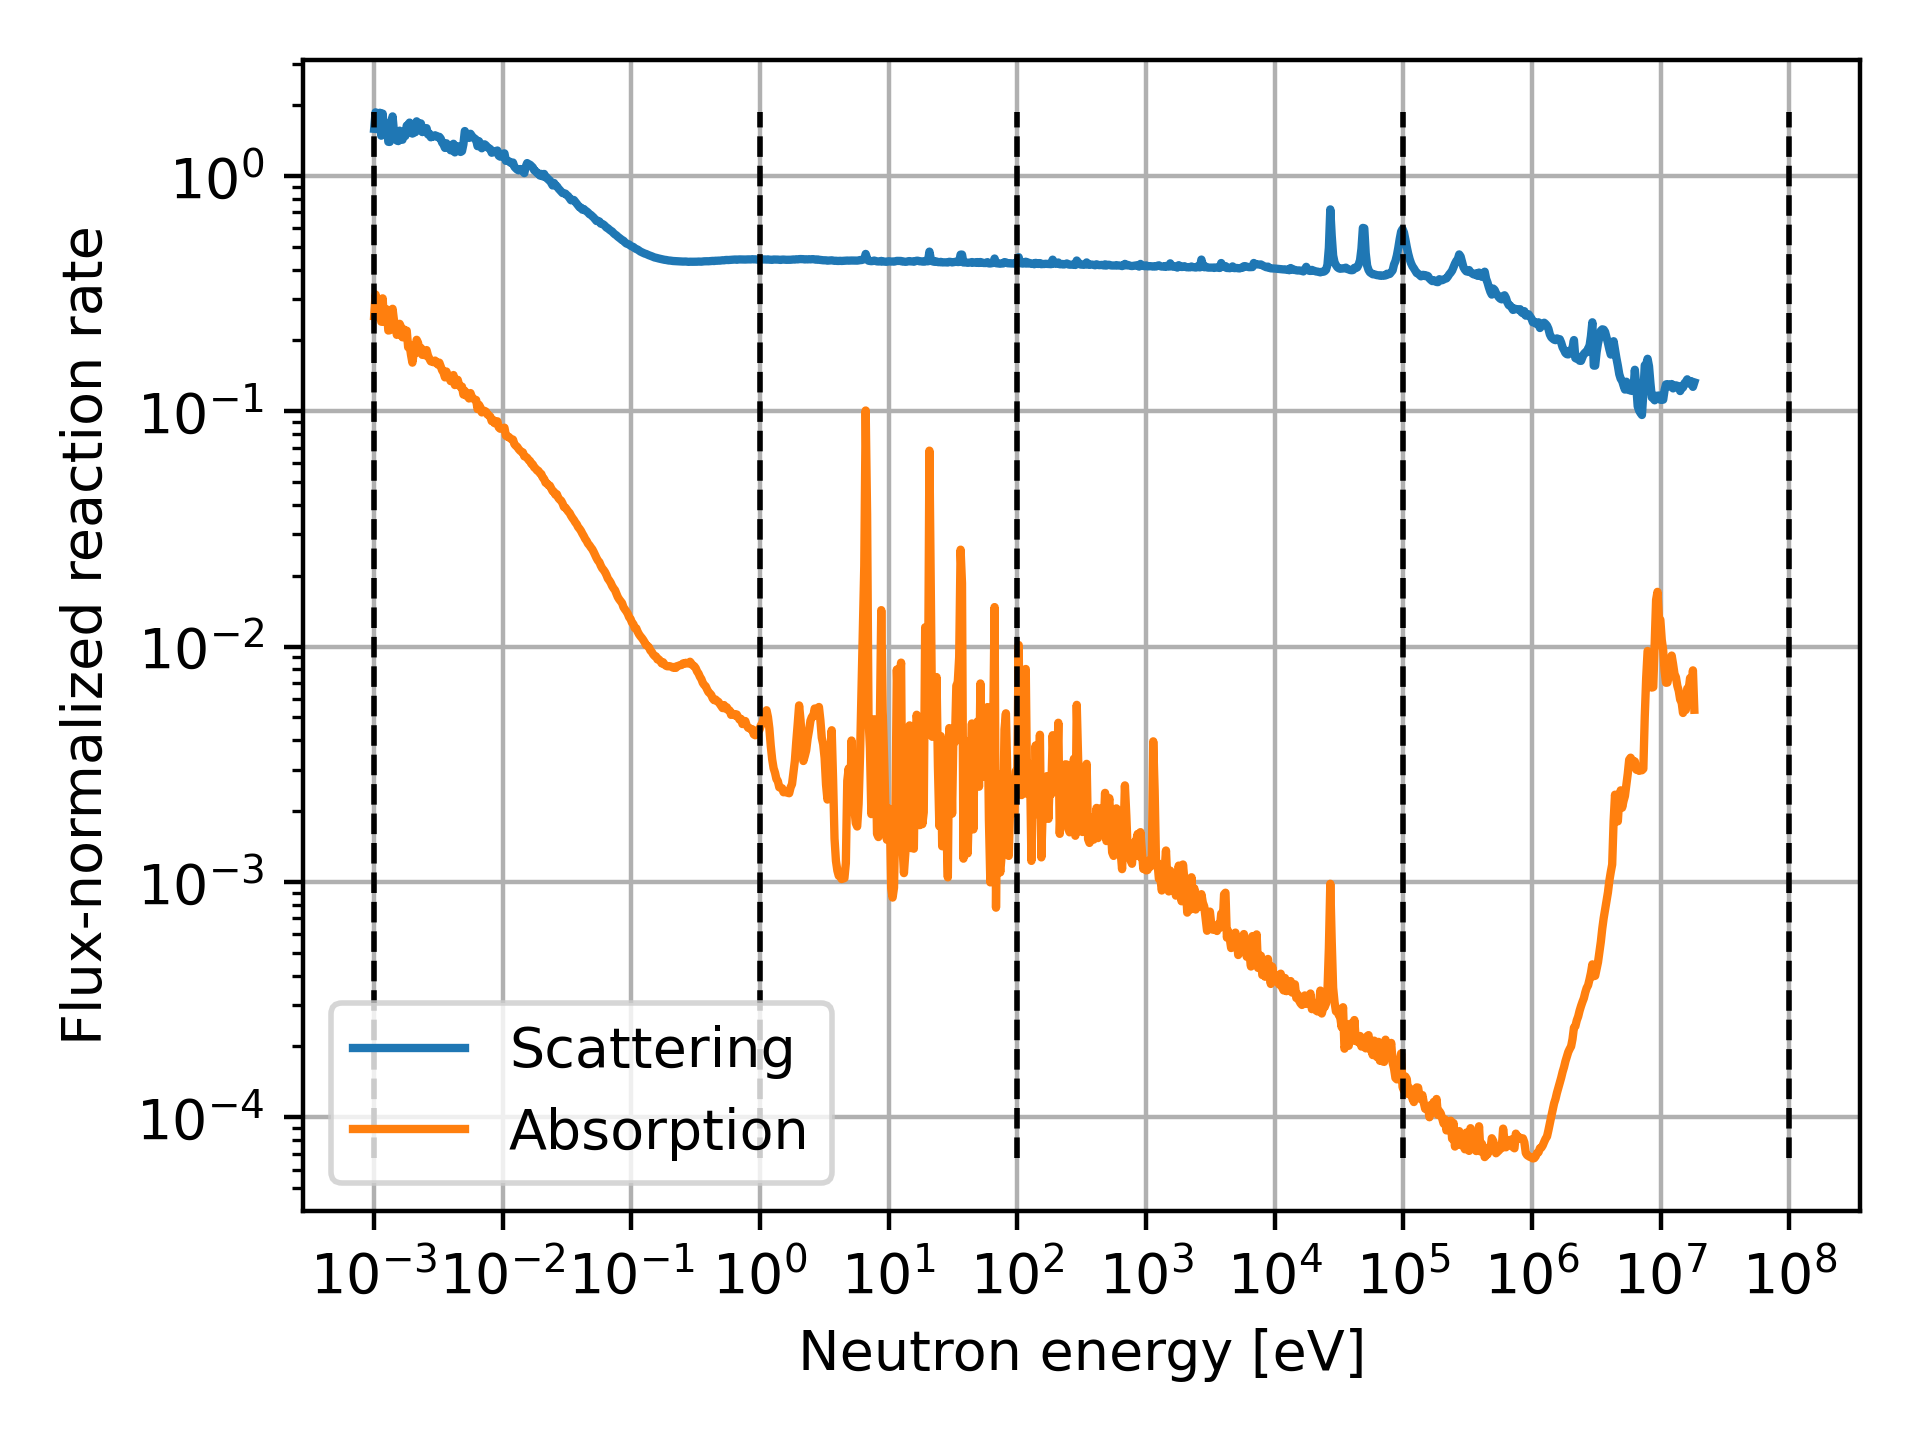
\includegraphics[width=\textwidth]{reaction}
    \caption{Flux-normalized scattering and absorption reaction rates}
    \label{fig:reaction}
  \end{subfigure}
  \caption{Neutron flux energy spectrum and reaction rates for Case 5a. The dotted vertical lines
  correspond to the discrete neutron energy group boundaries.}
  \label{fig:spec-reac}
\end{figure}
%
%\begin{table}[tb!]
%  \centering
%  \caption{Description of the 1-D Test Case Geometries.}
%  \begin{tabular}{l c c c}
%    \toprule
%    Cases & Ordered list of regions & Ordered list of interface x-coordinates & Left \& Right BCs\\
%    \midrule
%    Case 0 & Control rod, homogenized fuel-graphite lattice &
%    \bottomrule
%  \end{tabular}
%  \label{table:c0k}
%\end{table}

I ran all cases with four neutron energy groups. The list of energy group bounds are:
$E=[10^{-5}, 10^0, 10^2, 10^5, 10^8]$ eV. Figures \ref{fig:spectrum} and \ref{fig:reaction} show
how this energy group structure
partitions the neutron flux energy spectrum and neutron reaction rates. For this preliminary work,
the four-group structure is sufficient for showing different scattering and absorption trends of
slow, intermediate, and fast neutrons. I also ran all cases on OpenMC to generate the required
group constants and to assess the accuracy of the deterministic methods against OpenMC in
continuous-energy (OpenMC-CE) and multigroup (OpenMC-MG) modes. Table \ref{table:var} shows how the
position, direction of travel, neutron energy, and angle-dependence in $\Sigma_s$ are handled by
OpenMC and the deterministic methods. Comparing OpenMC-MG results with OpenMC-CE results allows us
to quantify errors arising from neutron energy group discretization and the scattering cross
section simplifications. Each Monte Carlo simulation ran on 25 inactive and 125 active cycles of
20,000 neutrons each, which sums up to 2.5 million tallied neutron histories.

\begin{table}[tb!]
  \centering
  \footnotesize
  \caption{Variable handling in OpenMC under continuous-energy (OpenMC-CE) and multigroup
  (OpenMC-MG) modes, and in the $S_N$ neutron transport, neutron diffusion, and hybrid
  $S_N$-diffusion methods. }
  \begin{tabular}{c c c c c c}
    \toprule
    Variable & OpenMC-CE & OpenMC-MG & $S_N$ Transport & Diffusion & Hybrid \\
    \midrule
    Position, $\bm{r}$ & Continuous & Continuous & Discrete & Discrete & Discrete \\
    Direction of travel, $\bm{\hat{\Omega}}$ & Continuous & Continuous & Discrete & N/A & N/A \\
    Energy, $E$ & Continuous & Discrete & Discrete & Discrete & Discrete \\
    Angle-dependence in $\Sigma_s$ & Continuous & 2nd Legendre moment & 2nd Legendre moment
    & N/A & N/A \\
    \bottomrule
  \end{tabular}
  \label{table:var}
\end{table}

\section{Simulation Parameters for Convergence} \label{sec:sim-param}

The convergence of the results depends mainly on the following simulation parameters: mesh size
($\Delta x$), convergence tolerance ($tol$), number of discrete ordinates ($N$), and the highest
order moment of the scattering cross sections ($L$). The last two parameters apply only to $S_N$
calculations. Table \ref{table:param} shows the values of simulation parameters applied to each
method for the 1-D test cases.

\begin{table}[tb!]
  \centering
  \footnotesize
  \caption{Simulation parameters applied to the neutron diffusion, $S_N$, and hybrid
  $S_N$-diffusion methods.}
  \begin{tabular}{c c c c}
    \toprule
    Parameter & $S_N$ Transport & Neutron Diffusion & Hybrid $S_N$-Diffusion \\
    \midrule
    Mesh size, $\Delta x$ [cm]        & 0.0125    & 0.0125    & 0.0125 \\[.2cm]
    \multirow{3}{*}{Convergence tolerance, $tol$}
                                      &           &           & Diffusion: $10^{-6}$ \\
                                      & $10^{-7}$ & $10^{-6}$ & $S_N$: $10^{-5}$ \\
                                      &           &           & Outer: $10^{-3}$ \\[.2cm]
    Discrete ordinates, $N$           & 8         & N/A       & 8 \\
    Highest moment of $\Sigma^{g'\rightarrow g}_s$, $L$
                                      & 2         & N/A       & 2 \\
    \bottomrule
  \end{tabular}
  \label{table:param}
\end{table}

The simulation parameters did not show any significant correlation in the convergence tests. All
three methods achieve reasonable convergence with $\Delta x=0.0125$ cm; halving the mesh size
causes less than $30\times10^{-5}$ change in $k$ for the neutron diffusion and hybrid methods and
less than $10^{-5}$ for the $S_8$ method. Further refinement of the $tol$, $N$, and $L$ parameters
result in less than $2\times10^{-5}$
change in $k$. The same $tol$ value applies to convergence checks for both $\phi$ and $k$ in all
three methods because the variables converge at similar rates. The hybrid method requires three
separate $tol$ values due to the inner and outer iterations. Notably, the hybrid method can reach
convergence with a larger $tol$ value for its $S_N$ sub-solver than the $tol$ value for the
standalone $S_N$ solver, which implies that $J$ and $\sfrac{d\phi}{dx}$ converge faster than $\phi$
because the \glspl{SVDC} depend on those variables instead of $\phi$. Consequently, the $S_N$
sub-solver requires much fewer iterations than the standalone $S_N$ solver. In combination with
restricting $S_N$ calculations to the correction region, the hybrid method saves significant
computation time compared to the standalone $S_N$ method.

The outer iterations
converge rapidly, so a $tol$ value of $10^{-3}$ is sufficient for convergence. The $\phi$ and $k$
relative error norms ($\epsilon$) in all test cases decreased by two orders of magnitude on
every outer iteration. For instance, Table \ref{table:epsilon} shows the $\epsilon$ values from the
hybrid method after every outer iteration for Case 5a. The $\epsilon$ values fall below
$10^{-5}$ by the 3rd and 4th iterations.

\begin{table}[tb!]
  \centering
  \footnotesize
  \caption{Relative error norm, $\epsilon$, values for $k$ and $\phi$ after each outer iteration in
    the hybrid $S_N$-diffusion method for Case 5a.}
  \begin{tabular}{c S[table-format=1.1e+1] S[table-format=1.1e+1]}
    \toprule
    Iteration   & {$\epsilon_k$}    & {$\epsilon_\phi$} \\
    \midrule
    1           & 1.6e-2            & 1.5e-2 \\
    2           & 5.0e-5            & 4.7e-5 \\
    3           & 1.4e-7            & 1.6e-7 \\
    4           & 3.5e-9            & 1.4e-8 \\
    \bottomrule
  \end{tabular}
  \label{table:epsilon}
\end{table}


\section{Results \& Discussion} \label{sec:prelim-results}

In this section, I compare neutronics parameters for all test cases calculated from
the OpenMC and deterministic methods. I refer to the OpenMC calculations under continuous-energy
and multigroup modes as OpenMC-CE and OpenMC-MG, respectively. I did not apply the hybrid method to
Cases 1a, 1b, 4a, 4b, and 5b, which serve as reference cases for how much the neutron diffusion
method underperforms when control rod regions are present in the other cases.

\subsection{Comparison of Multiplication factors, $k$}

Tables \ref{table:ck1} and \ref{table:ck2} show all test case $k$ estimates from the OpenMC and
deterministic methods. The tables also include statistical uncertainties for the OpenMC
$k$ estimates.

All five methods generally show reasonable agreement within each test case. The differences between
the OpenMC-CE and OpenMC-MG $k$ estimates vary significantly from 0.00018 in Case 1a to 0.01622 in
Case 4b. These Monte Carlo methods exhibit more significant differences in cases
with vacuum boundary conditions (e.g., Cases 1b, 2b, 3b, 4b, 5a, 5b). These differences imply that
the neutron energy discretization scheme must be revised to capture neutron leakage rates
accurately. Beyond this preliminary study, I will explore better discrete energy group structures
for further neutronics analyses of graphite-moderated \glspl{MSR}. For the rest of this
section, I compare the $k$ estimates of the deterministic methods with OpenMC-MG.

\begin{table}[htb!]
  \centering
  \footnotesize
  \caption{Multiplication factor $k$ estimates for Cases 1a, 1b, 2a, 2b, 3a, and 3b from the
    OpenMC-CE, OpenMC-MG, $S_8$ neutron transport, neutron diffusion, and hybrid $S_N$-diffusion
    methods.}
  \begin{tabular}{c S[table-format=1.5(2)] S[table-format=1.5(2)] S[table-format=1.5(2)]
  S[table-format=1.5(2)] S[table-format=1.5(2)] S[table-format=1.5(2)]}
    \toprule
    \multirow{2}{*}{\textbf{Method}} &
    \multicolumn{6}{c}{\textbf{Multiplication factor,} $\bm{k}$} \\
    \cmidrule{2-7}
    & {\textbf{Case 1a}} & {\textbf{Case 1b}} & {\textbf{Case 2a}} &
    {\textbf{Case 2b}} & {\textbf{Case 3a}} & {\textbf{Case 3b}} \\
    \midrule
    OpenMC-CE & 1.60033(56) & 1.16749(60) & 1.20666(66) & 0.69499(47) & 1.19908(63) & 0.68565(53)\\
    OpenMC-MG & 1.60015(33) & 1.18104(54) & 1.20570(66) & 0.70539(50) & 1.19976(48) & 0.69730(50)\\
    $S_8$     & 1.60035     & 1.18068     & 1.20596     & 0.70470     & 1.19968     & 0.69652    \\
    Diffusion & 1.60036     & 1.17932     & 1.19709     & 0.69274     & 1.19064     & 0.68450    \\
    Hybrid    & {N/A}       & {N/A}       & 1.20630     & 0.70387     & 1.20004     & 0.69568    \\
    \bottomrule
  \end{tabular}
  \label{table:ck1}
\end{table}
%
\begin{table}[htb!]
  \centering
  \footnotesize
  \caption{Multiplication factor $k$ estimates for Cases 4a, 4b, 5a, and 5b from the OpenMC-CE,
    OpenMC-MG, $S_8$ neutron transport, neutron diffusion, and hybrid $S_N$-diffusion methods.}
  \begin{tabular}{c S[table-format=1.5(2)] S[table-format=1.5(2)] S[table-format=1.5(2)]
    S[table-format=1.5(2)]}
    \toprule
    \multirow{2}{*}{\textbf{Method}} &
    \multicolumn{4}{c}{\textbf{Multiplication factor,} $\bm{k}$} \\
    \cmidrule{2-5}
    & {\textbf{Case 4a}} & {\textbf{Case 4b}} & {\textbf{Case 5a}} &
    {\textbf{Case 5b}} \\
    \midrule
    OpenMC-CE & 1.64506(53) & 1.19116(63) & 0.70352(64) & 1.16832(58) \\
    OpenMC-MG & 1.64355(37) & 1.20738(63) & 0.71396(50) & 1.18204(53) \\
    $S_8$     & 1.64376     & 1.20744     & 0.71379     & 1.18218     \\
    Diffusion & 1.64355     & 1.20811     & 0.70524     & 1.18274     \\
    Hybrid    & {N/A}       & {N/A}       & 0.71673     & {N/A}       \\
    \bottomrule
  \end{tabular}
  \label{table:ck2}
\end{table}
%
\begin{table}[htb!]
  \centering
  \footnotesize
  \caption{Differences in $k$ estimates for Cases 1a, 1b, 2a, 2b, 3a, and 3b for the $S_8$ neutron
    transport, neutron diffusion, and hybrid $S_N$-diffusion methods relative to OpenMC-MG.}
  \begin{tabular}{c S[table-format=+1.5(2)] S[table-format=+1.5(2)] S[table-format=+1.5(2)]
      S[table-format=+1.5(2)] S[table-format=+1.5(2)] S[table-format=+1.5(2)]}
    \toprule
    \multirow{2}{*}{\textbf{Method}} & \multicolumn{6}{c}{$\bm{k-k_{MG}}$} \\
    \cmidrule{2-7}
    & {\textbf{Case 1a}} & {\textbf{Case 1b}} & {\textbf{Case 2a}} &
    {\textbf{Case 2b}} & {\textbf{Case 3a}} & {\textbf{Case 3b}} \\
    \midrule
    $S_8$     & +0.00020(33) & -0.00036(54) & +0.00026(66) & -0.00069(50) & -0.00008(48) & -0.00078(50) \\
    Diffusion & +0.00021(33) & -0.00172(54) & -0.00861(66) & -0.01265(50) & -0.00912(48) & -0.01280(50) \\
    Hybrid    & {N/A}        & {N/A}        & +0.00060(66) & -0.00152(50) & +0.00028(48) & -0.00162(50) \\
    \bottomrule
  \end{tabular}
  \label{table:ckdiff1}
\end{table}
%
\begin{table}[htb!]
  \centering
  \footnotesize
  \caption{Differences in $k$ estimates for Cases 4a, 4b, 5a, and 5b for the $S_8$ neutron
    transport, neutron diffusion, and hybrid $S_N$-diffusion methods relative to OpenMC-MG.}
  \begin{tabular}{c S[table-format=+1.5(2)] S[table-format=+1.5(2)] S[table-format=+1.5(2)]
    S[table-format=+1.5(2)]}
    \toprule
    \multirow{2}{*}{\textbf{Method}} & \multicolumn{4}{c}{$\bm{k-k_{MG}}$} \\
    \cmidrule{2-5}
    & {\textbf{Case 4a}} & {\textbf{Case 4b}} & {\textbf{Case 5a}} &
    {\textbf{Case 5b}} \\
    \midrule
    $S_8$     & +0.00021(37) & +0.00006(63) & -0.00017(50) & -0.00027(53) \\
    Diffusion & +0.00000(37) & +0.00073(63) & -0.00872(50) & +0.00277(53) \\
    Hybrid    & {N/A}        & {N/A}        & +0.00070(50) & {N/A}    \\
    \bottomrule
  \end{tabular}
  \label{table:ckdiff2}
\end{table}
%
\begin{table}[tb!]
  \centering
  \footnotesize
  \caption{Control rod worths calculated as changes in the reactivity between Case 5a and 5b for
    the OpenMC continuous-energy and multigroup mode calculations, and the $S_8$ neutron transport,
  neutron diffusion, and hybrid $S_N$-diffusion methods.}
  \begin{tabular}{c S}
    \toprule
    \multirow{2}{*}{\textbf{Method}} & {\textbf{Control rod worth}} \\
                                     & {$\bm{\rho_{(5b)}-\rho_{(5a)}}$} \\
    \midrule
    OpenMC-CE & 0.56549(213) \\
    OpenMC-MG & 0.55464(176) \\
    $S_8$     & 0.55507 \\
    Diffusion & 0.57246 \\
    Hybrid    & 0.54974 \\
    \bottomrule
  \end{tabular}
  \label{table:rod-worth}
\end{table}

Tables \ref{table:ckdiff1} and \ref{table:ckdiff2} show the differences in $k$ between OpenMC-MG
and deterministic methods. The $k$ estimates from the $S_8$ neutron transport method show
good agreement, with the estimates from OpenMC-MG with all pairs of $k$ values falling within
1-2 standard deviations of each other. The only significant difference in implementation between
the OpenMC-MG and $S_8$ methods is the discretization of the direction of travel variable
$\hat{\Omega}$. The flux distributions exhibit more apparent differences, will be discussed in the
following subsection. Nevertheless, the $S_8$ method is sufficiently accurate and consistent for
modeling this graphite-moderated system with control rods.

As expected, the neutron diffusion method performs significantly worse than the $S_8$ method in
Cases 2, 3, and 5a, containing control rod regions. It deviates from the OpenMC-MG $k$
estimate by up to -0.01280 in Case 3b compared to -0.00078 for the $S_8$ method. The hybrid method
effectively improves the $k$ estimate to -0.00162 of the
OpenMC-MG method for Case 3b. The hybrid method also appreciably improved the accuracy in all
other applied cases.

In a time-dependent multiphysics simulation involving rod
insertion or withdrawal, the control rod worth determines the change in reactivity and the
subsequent effects on the neutron flux and temperature distribution. I calculated the control rod
worth by taking the change in reactivity $\rho$ between Case 5a and 5b for all five methods, as
shown in Table \ref{table:rod-worth}. The formula for $\rho$ is given as
%
\begin{align}
  \rho =& \frac{k-1}{k}.
\end{align}
%
I took the $k$ estimate from the neutron diffusion method in Case 5b as the reference non-inserted
case for the control rod worth calculation for the hybrid method. Compared with OpenMC-MG, the
control rod worth from the neutron diffusion method deviates the most by 1782 pcm (percent mille)
as opposed to 43 pcm and -490 pcm by the $S_8$ and hybrid methods, respectively.

\subsection{Comparison of Neutron Flux Distributions, $\phi$}

This section focuses on the neutron flux distributions in Cases 3b and 5a, representing the most
complex geometries with homogeneous and lattice fuel-graphite regions. I sampled the flux
distributions in OpenMC-CE and OpenMC-MG across coarser $0.1$-cm intervals to reduce the
statistical uncertainties of each flux reading.

\begin{figure}[htb!]
  \centering
  \begin{subfigure}[t]{.49\textwidth}
    \centering
    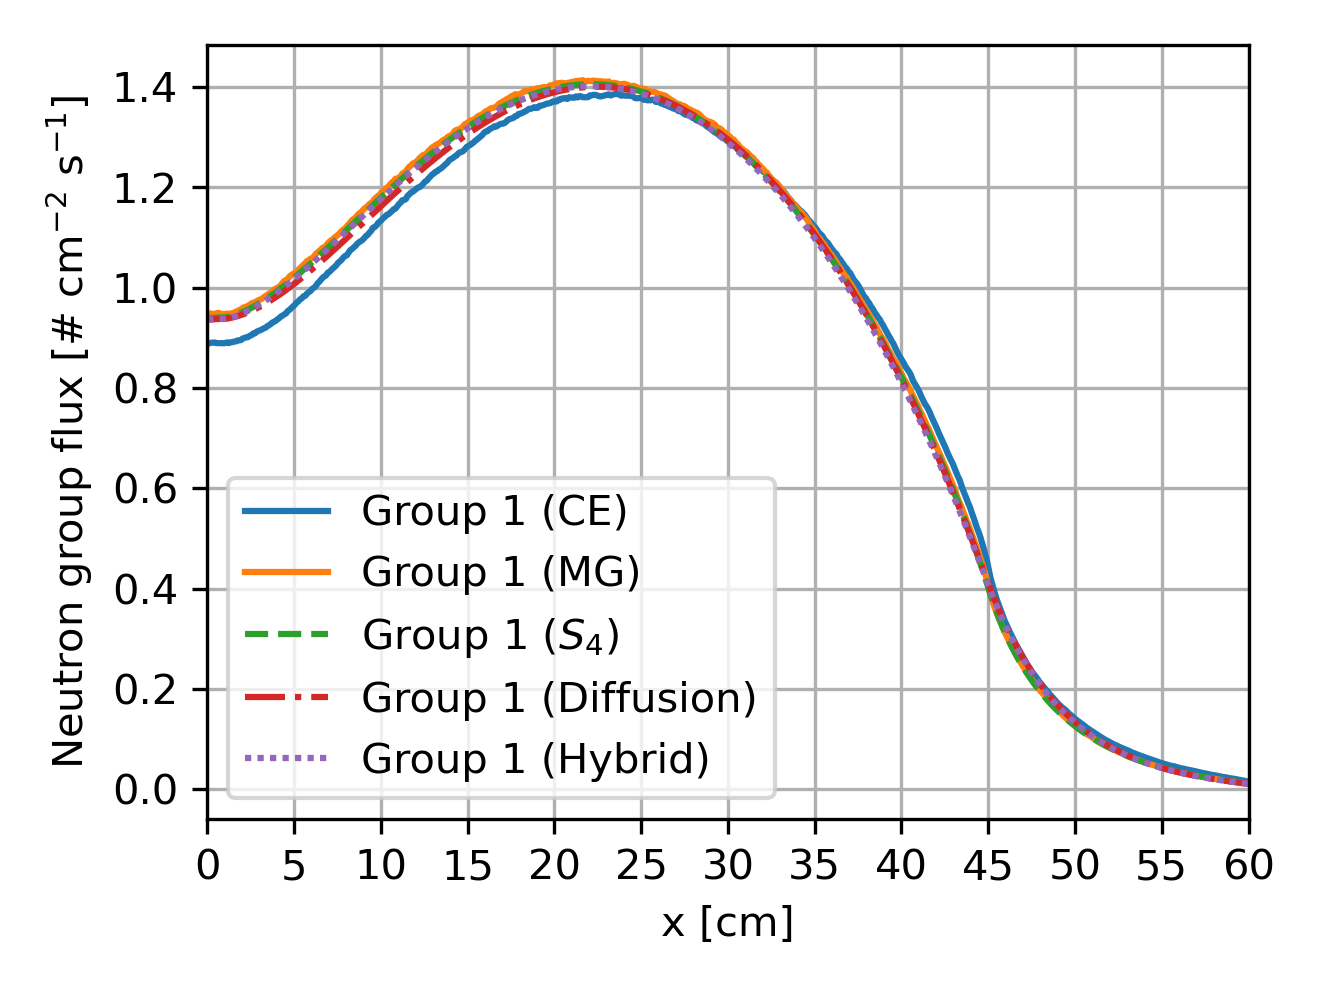
\includegraphics[width=\textwidth]{case-3b-group-1-flux}
    \caption{Group 1}
    \label{fig:c3bg1}
  \end{subfigure}
  \hfill
  \begin{subfigure}[t]{.49\textwidth}
    \centering
    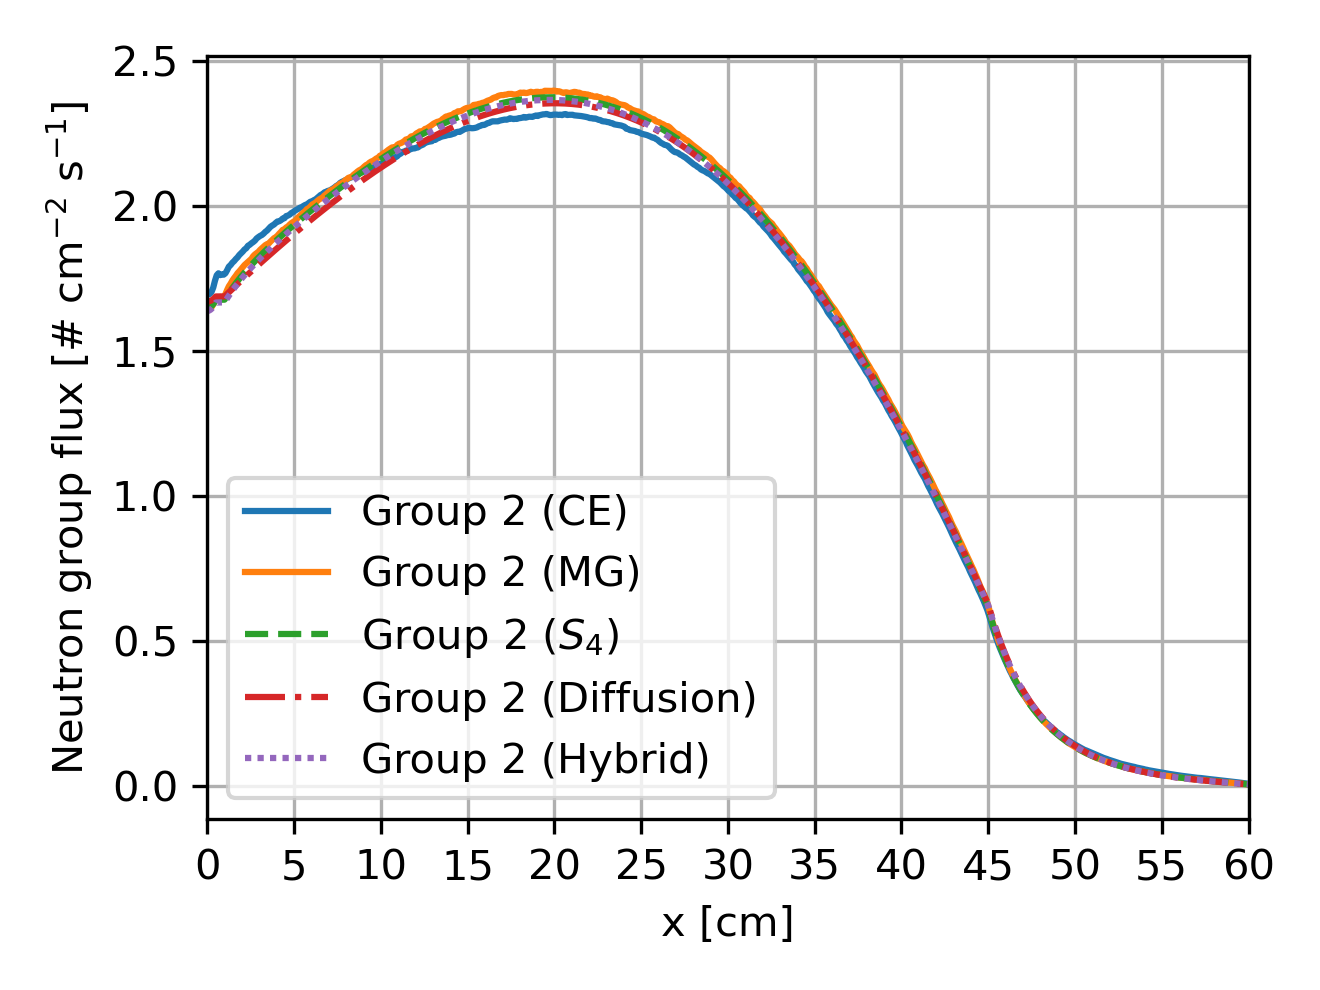
\includegraphics[width=\textwidth]{case-3b-group-2-flux}
    \caption{Group 2}
    \label{fig:c3bg2}
  \end{subfigure}
  \begin{subfigure}[t]{.49\textwidth}
    \centering
    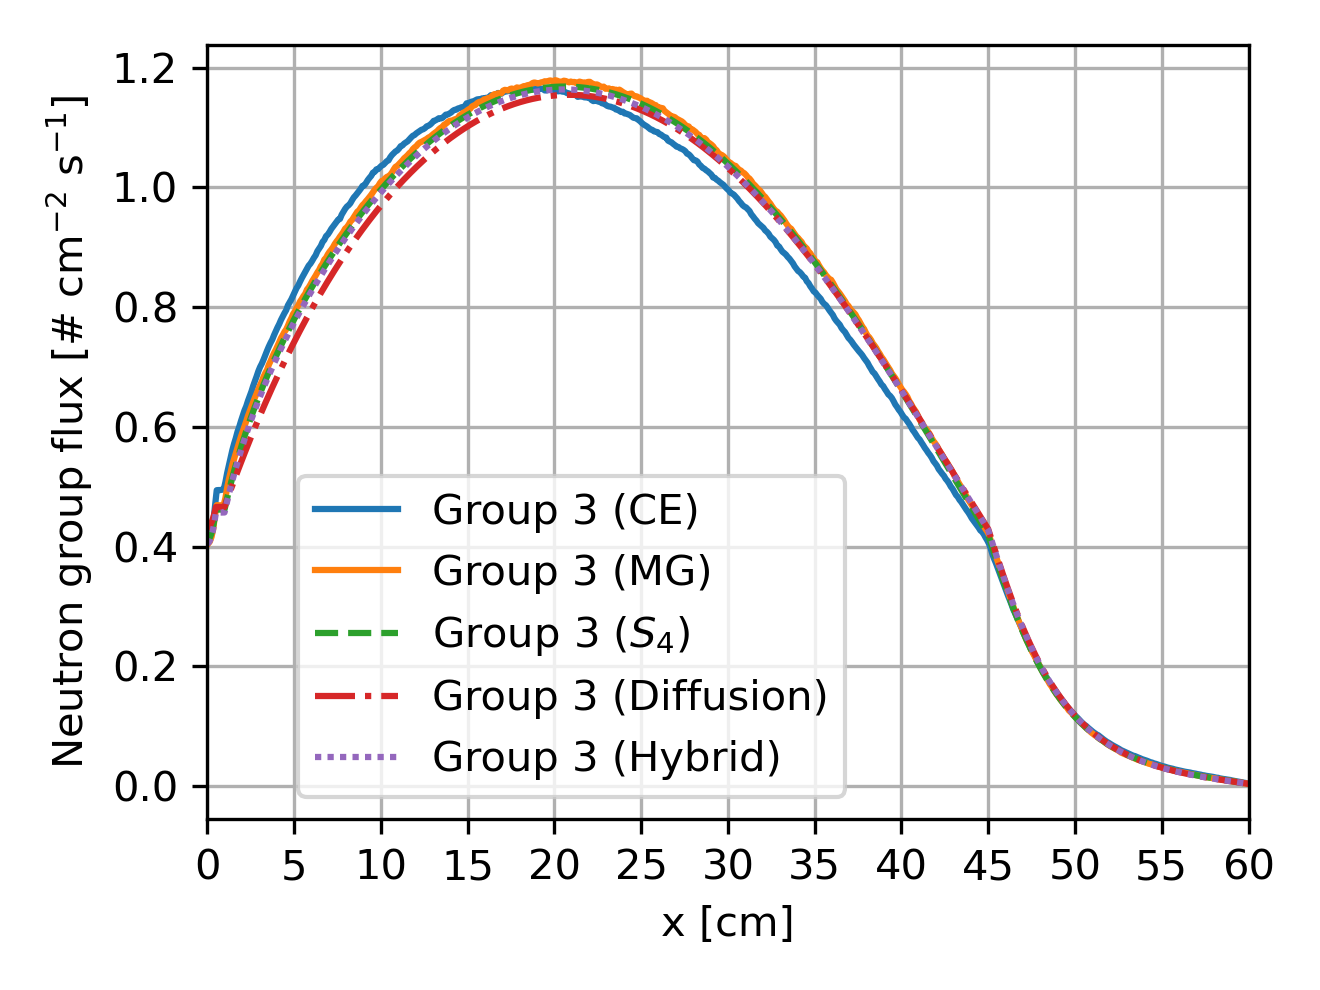
\includegraphics[width=\textwidth]{case-3b-group-3-flux}
    \caption{Group 3}
    \label{fig:c3bg3}
  \end{subfigure}
  \hfill
  \begin{subfigure}[t]{.49\textwidth}
    \centering
    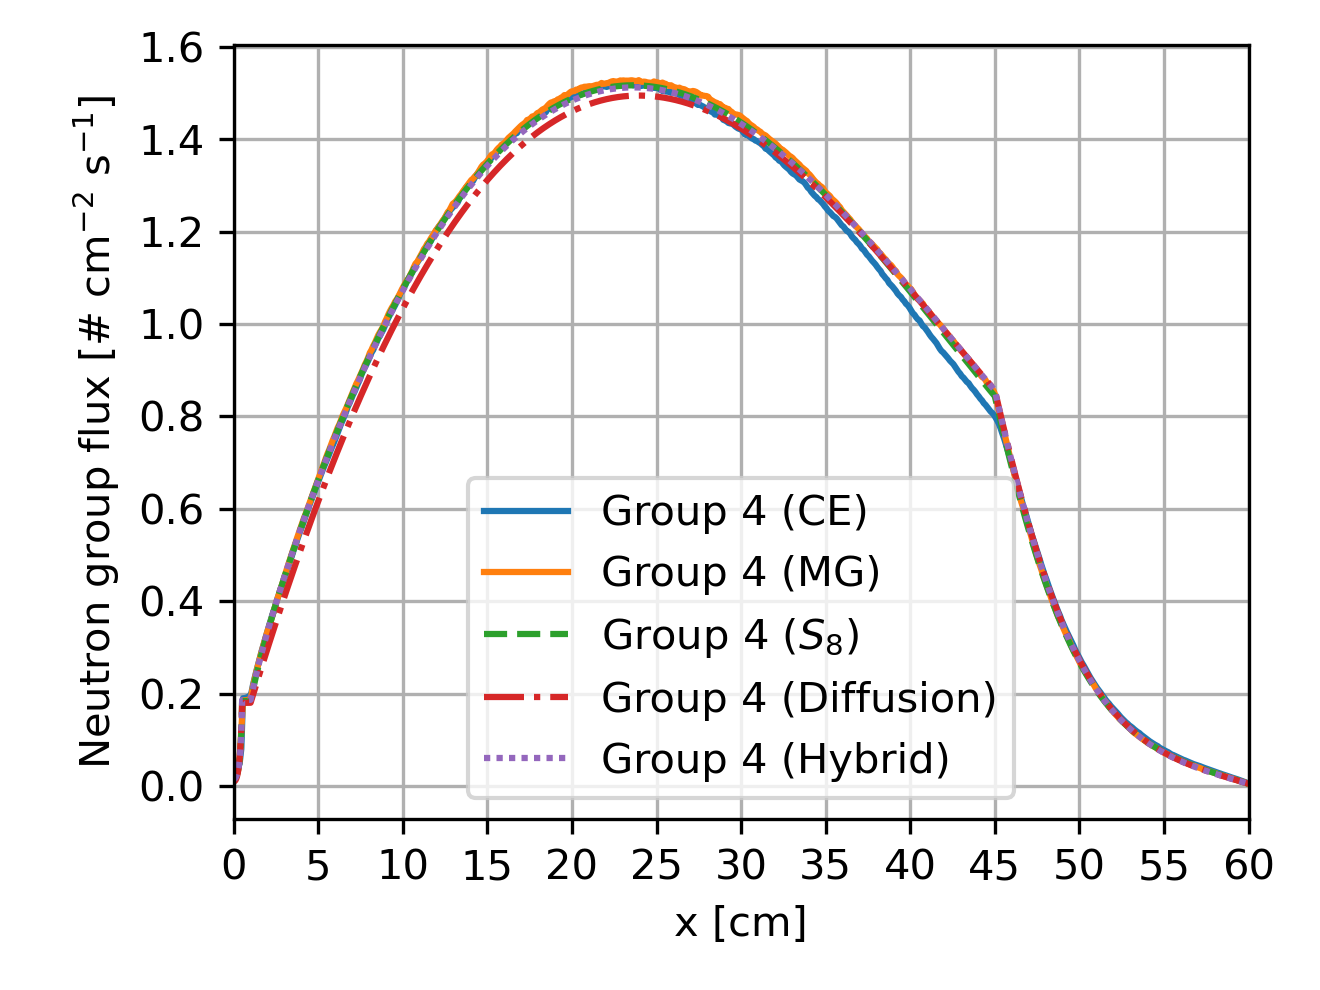
\includegraphics[width=\textwidth]{case-3b-group-4-flux}
    \caption{Group 4}
    \label{fig:c3bg4}
  \end{subfigure}
  \caption{Neutron group flux distributions for Case 3b from OpenMC-CE, OpenMC-MG, $S_8$, neutron
  diffusion, and hybrid methods.}
  \label{fig:c3bflux}
\end{figure}

Figure \ref{fig:c3bflux} shows the neutron flux distributions for groups 1 to 4. Notably, the
OpenMC-CE flux distribution is the most dissimilar, likely due to
the inadequate neutron energy discretization scheme. Consequently, I compared the
deterministic methods with OpenMC-MG to eliminate energy discretization errors. Figure
\ref{fig:c3bfluxe} shows the relative differences in the flux distributions from $S_8$, neutron
diffusion, and hybrid methods with respect to OpenMC-MG. The neutron diffusion method
performs worse than $S_8$, especially near the control rod region between $x=0$ cm and $x=20$ cm
for the slower group 3 and 4 neutron flux. Although the control rod region spans between $x=0$ cm
and $x=0.5$ cm only, it induces strong flux gradients in its vicinity, thus rendering the neutron
diffusion method less valid. The hybrid method significantly improves all four
group fluxes in this region. Beyond $x=40$ cm, the neutron diffusion and hybrid methods produce
similar flux error distributions due to the influence of the material interface between the
fuel-graphite and reflector regions.

\begin{figure}[htb!]
  \centering
  \begin{subfigure}[t]{.49\textwidth}
    \centering
    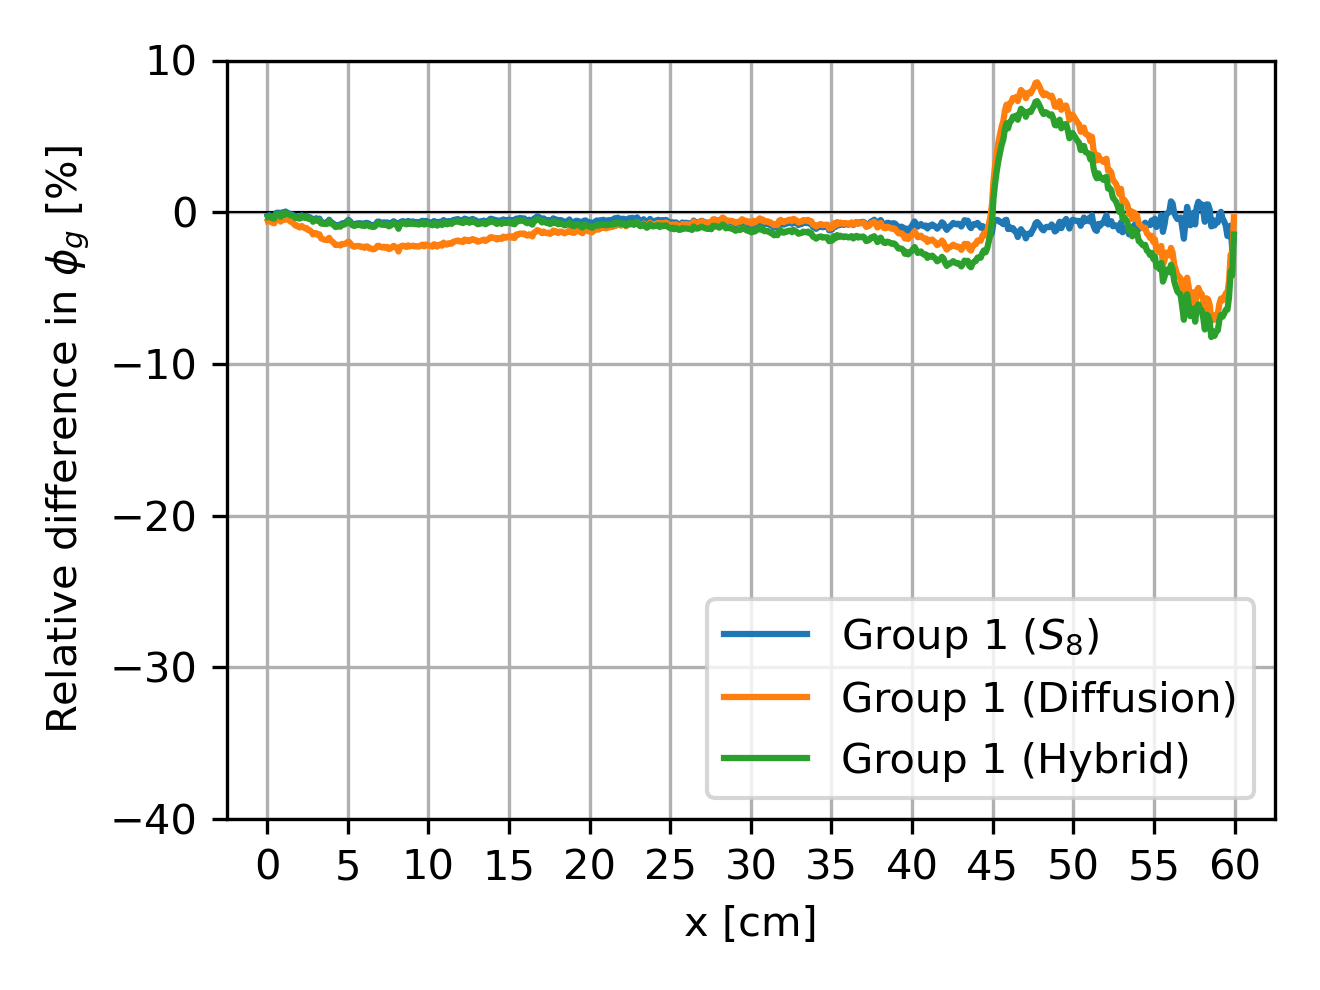
\includegraphics[width=\textwidth]{case-3b-group-1-flux-error}
    \caption{Group 1}
    \label{fig:c3bg1e}
  \end{subfigure}
  \hfill
  \begin{subfigure}[t]{.49\textwidth}
    \centering
    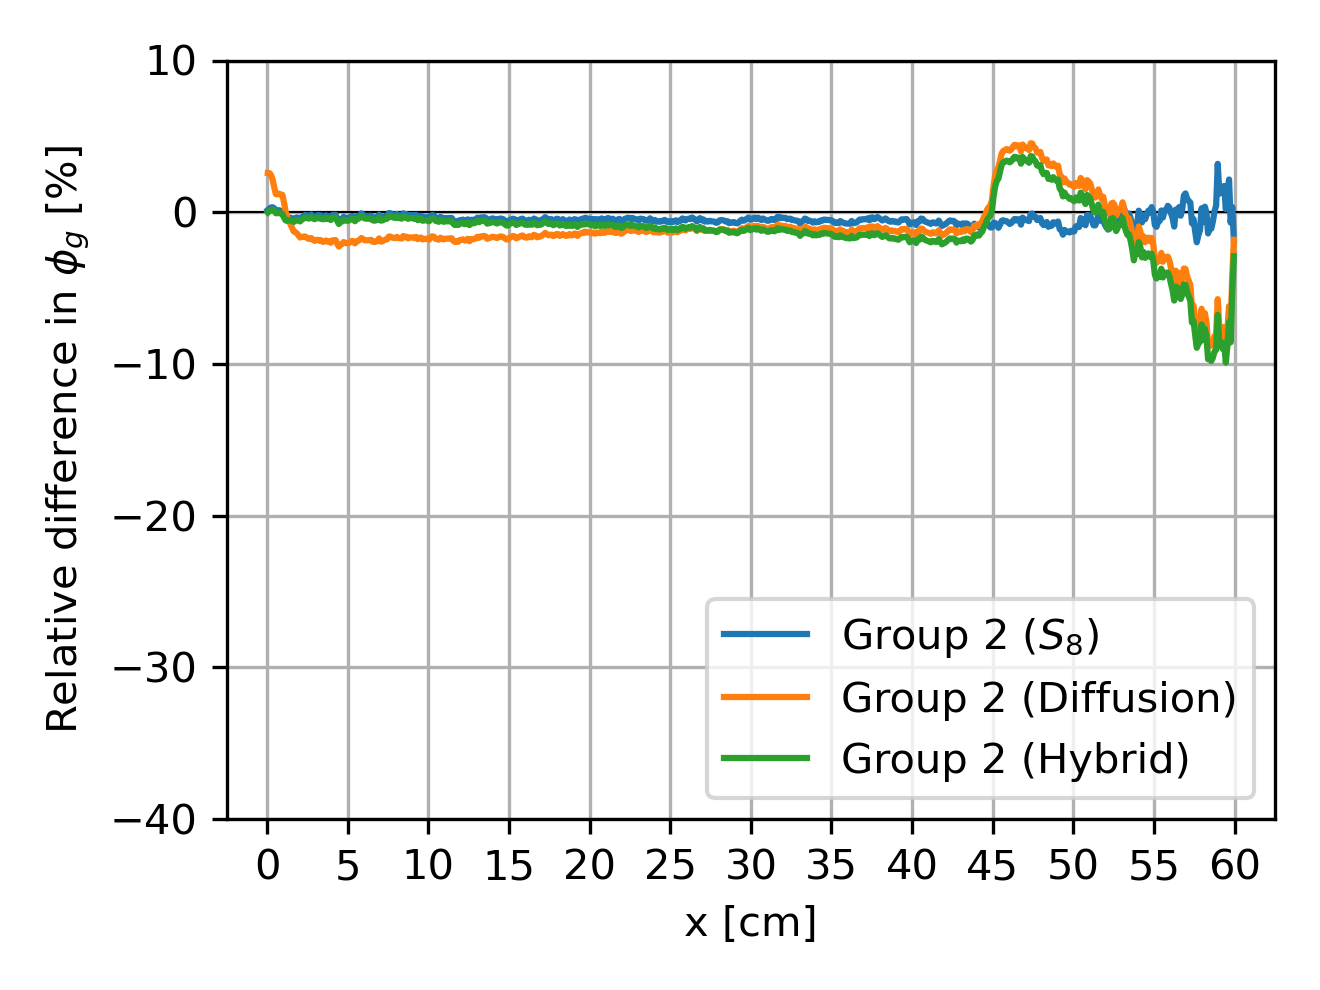
\includegraphics[width=\textwidth]{case-3b-group-2-flux-error}
    \caption{Group 2}
    \label{fig:c3bg2e}
  \end{subfigure}
  \begin{subfigure}[t]{.49\textwidth}
    \centering
    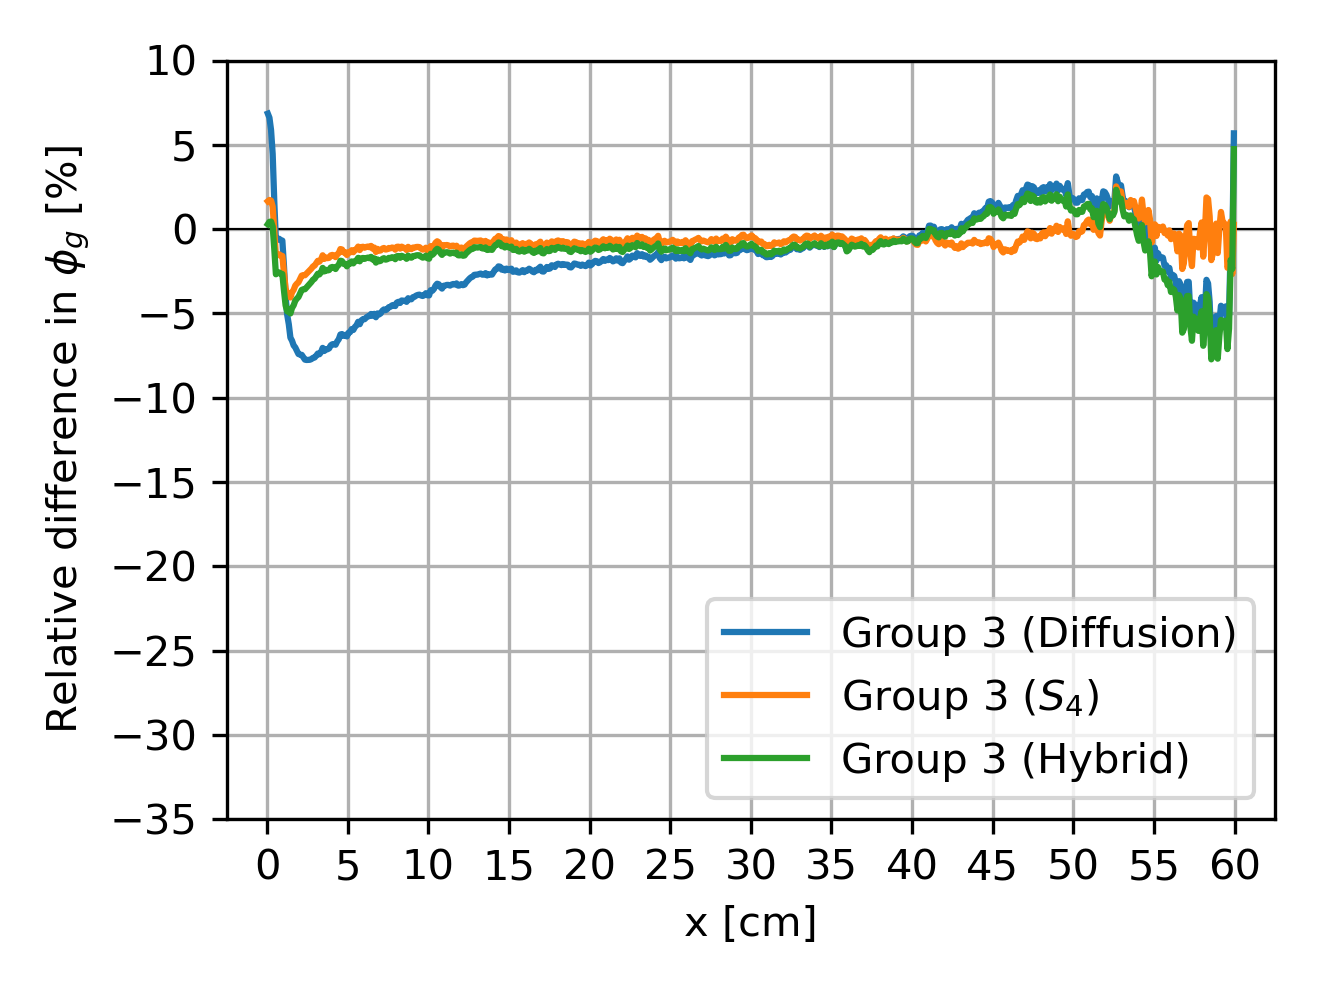
\includegraphics[width=\textwidth]{case-3b-group-3-flux-error}
    \caption{Group 3}
    \label{fig:c3bg3e}
  \end{subfigure}
  \hfill
  \begin{subfigure}[t]{.49\textwidth}
    \centering
    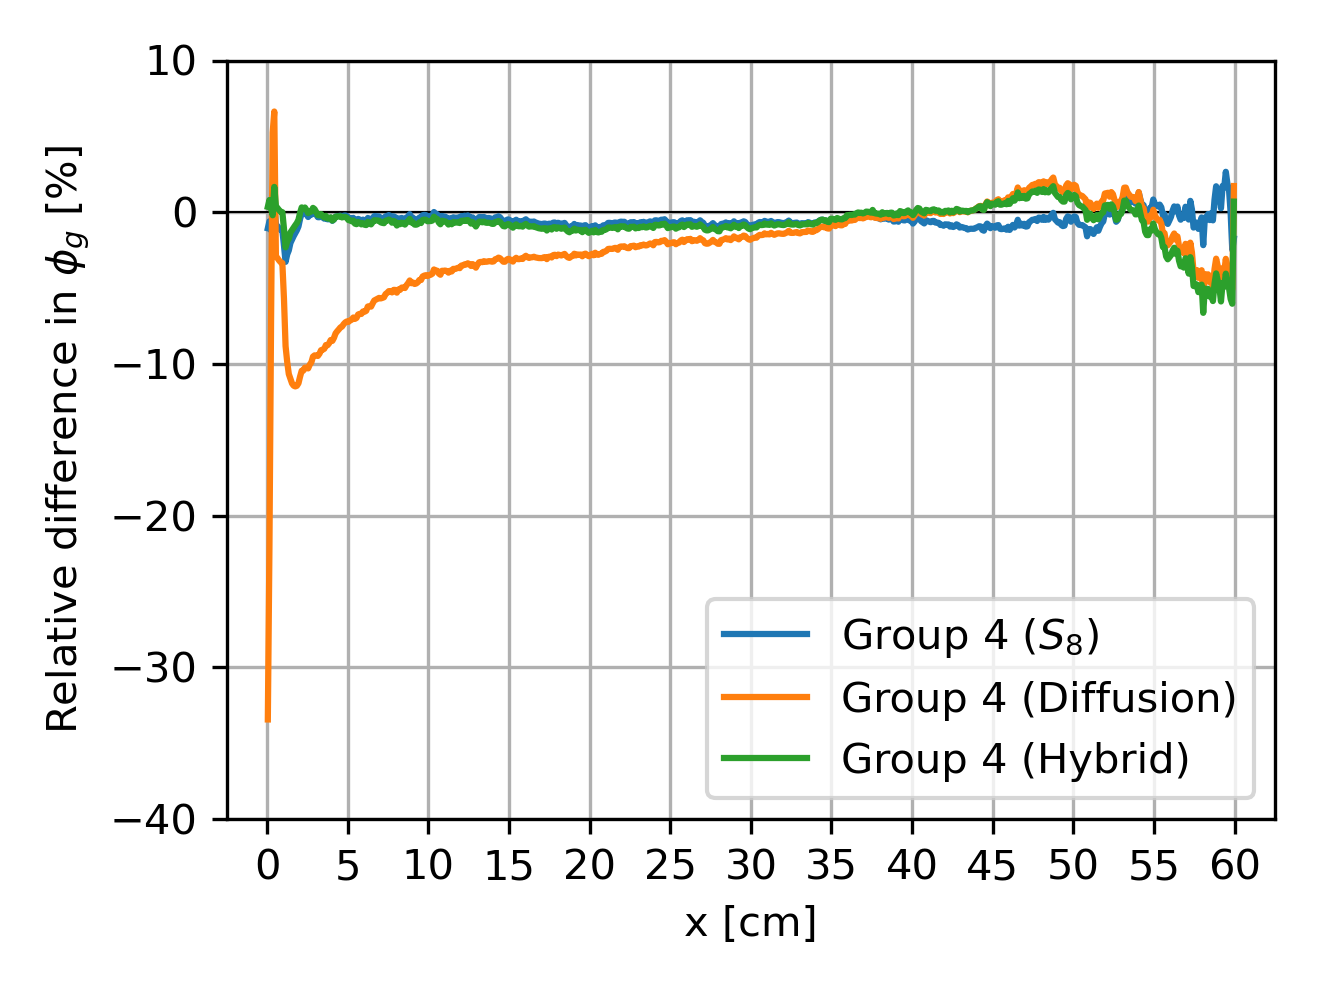
\includegraphics[width=\textwidth]{case-3b-group-4-flux-error}
    \caption{Group 4}
    \label{fig:c3bg4e}
  \end{subfigure}
  \caption{Relative differences of the neutron group flux distributions for Case 3b from the $S_8$,
    neutron diffusion, and hybrid methods with respect to OpenMC-MG.}
  \label{fig:c3bfluxe}
\end{figure}

For a quantitative assessment, I defined the normalized flux error $\varepsilon$ (not to be
confused with relative error norm $\epsilon$) for each energy group with respect to the OpenMC-MG
flux distribution using a normalized Frobenius/Euclidean norm formula given as
%
\begin{align}
  \varepsilon_g =& \frac{\lVert\sum^I_{i=1}\phi_{g,i} - \phi^{MG}_{g,i}\rVert_F}
  {\lVert\sum^I_{i=1}\phi^{MG}_{g,i}\rVert_F} =
  \frac{\left[\sum^I_{i=1}\lvert\phi_{g,i} - \phi^{MG}_{g,i}\rvert^2 \right]^{\sfrac{1}{2}}}
  {\left[\sum^I_{i=1}\lvert\phi^{MG}_{g,i}\rvert^2\right]^{\sfrac{1}{2}}}
\end{align}
%
I integrated on the fine flux distributions over 0.1-cm intervals from $S_8$, neutron diffusion,
and hybrid methods to match the 0.1-cm intervals of the OpenMC-MG flux distribution. Table
\ref{table:c3berror} shows the $\varepsilon$ values for the deterministic methods. As expected,
the hybrid method produces smaller flux error norms than the neutron diffusion method. The
improvements are more pronounced for group 3 and 4 fluxes than group 1 and 2 fluxes.
%
\begin{table}[tb!]
  \centering
  \footnotesize
  \caption{Normalized flux error $\varepsilon$ for Case 3b from the $S_8$, neutron diffusion, and
    hybrid methods with respect to OpenMC-MG.}
  \begin{tabular}{c S S S S}
    \toprule
    {\multirow{2}{*}{\textbf{Method}}} &
    \multicolumn{4}{c}{\textbf{Normalized flux error,} $\bm{\varepsilon_g}$} \\
    \cmidrule{2-5}
    & {\textbf{Group 1}} & {\textbf{Group 2}} & {\textbf{Group 3}} &
    {\textbf{Group 4}} \\
    \midrule
    $S_8$     & 0.0066 & 0.0048 & 0.0058 & 0.0067 \\
    Diffusion & 0.0144 & 0.0147 & 0.0258 & 0.0267 \\
    Hybrid    & 0.0122 & 0.0099 & 0.0087 & 0.0084 \\
    \bottomrule
  \end{tabular}
  \label{table:c3berror}
\end{table}

Case 5a introduces significant geometrical heterogeneity from the fuel-graphite lattice region.
The heterogeneity is very apparent from the flux distributions in Figure \ref{fig:c5aflux}. The
OpenMC Monte
Carlo methods captured the fluctuations in the flux through their continuous angle variable as
opposed to the $S_8$, neutron diffusion, and hybrid methods. The group 1 flux peaks are notably
pronounced since all fission neutrons are born in the fuel region, with the majority in group 1.
Figure \ref{fig:c5afluxe} shows the relative differences in flux for the $S_8$, neutron diffusion,
and hybrid methods relative to OpenMC-MG. All three methods show regular fluctuations in the
relative flux differences corresponding to the fuel-graphite lattice. The $S_8$ method generally
deviates the least from OpenMC-MG, while the neutron diffusion method exhibits
significant flux deviations near the control rod region prior to $x=20$ cm and the material
interface between the fuel and reflector regions beyond $x=40$ cm.

\begin{figure}[htb!]
  \centering
  \begin{subfigure}[t]{.49\textwidth}
    \centering
    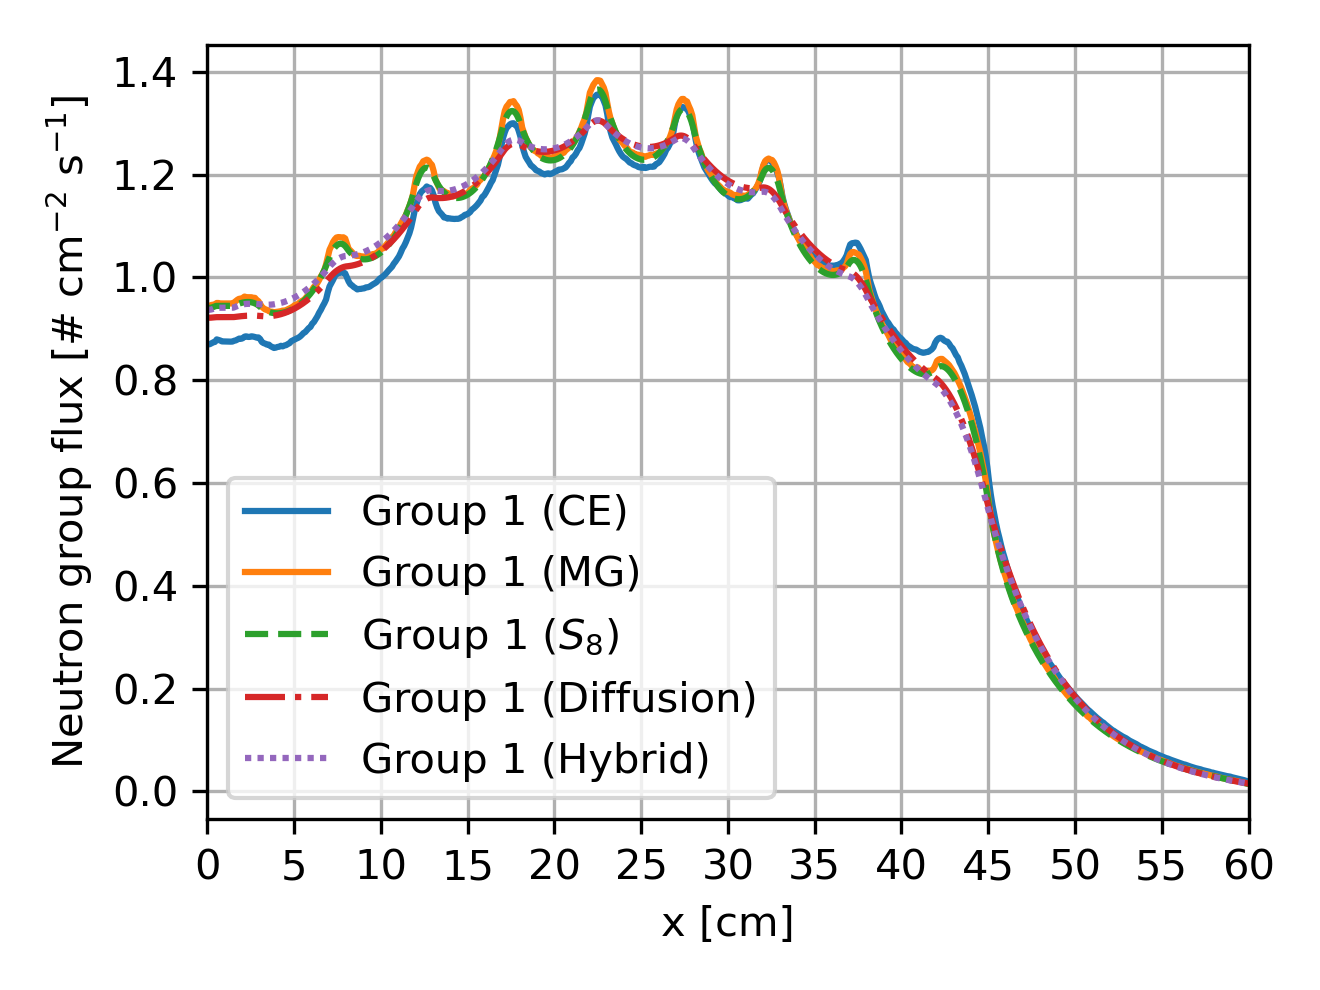
\includegraphics[width=\textwidth]{case-5a-group-1-flux}
    \caption{Group 1}
    \label{fig:c5ag1}
  \end{subfigure}
  \hfill
  \begin{subfigure}[t]{.49\textwidth}
    \centering
    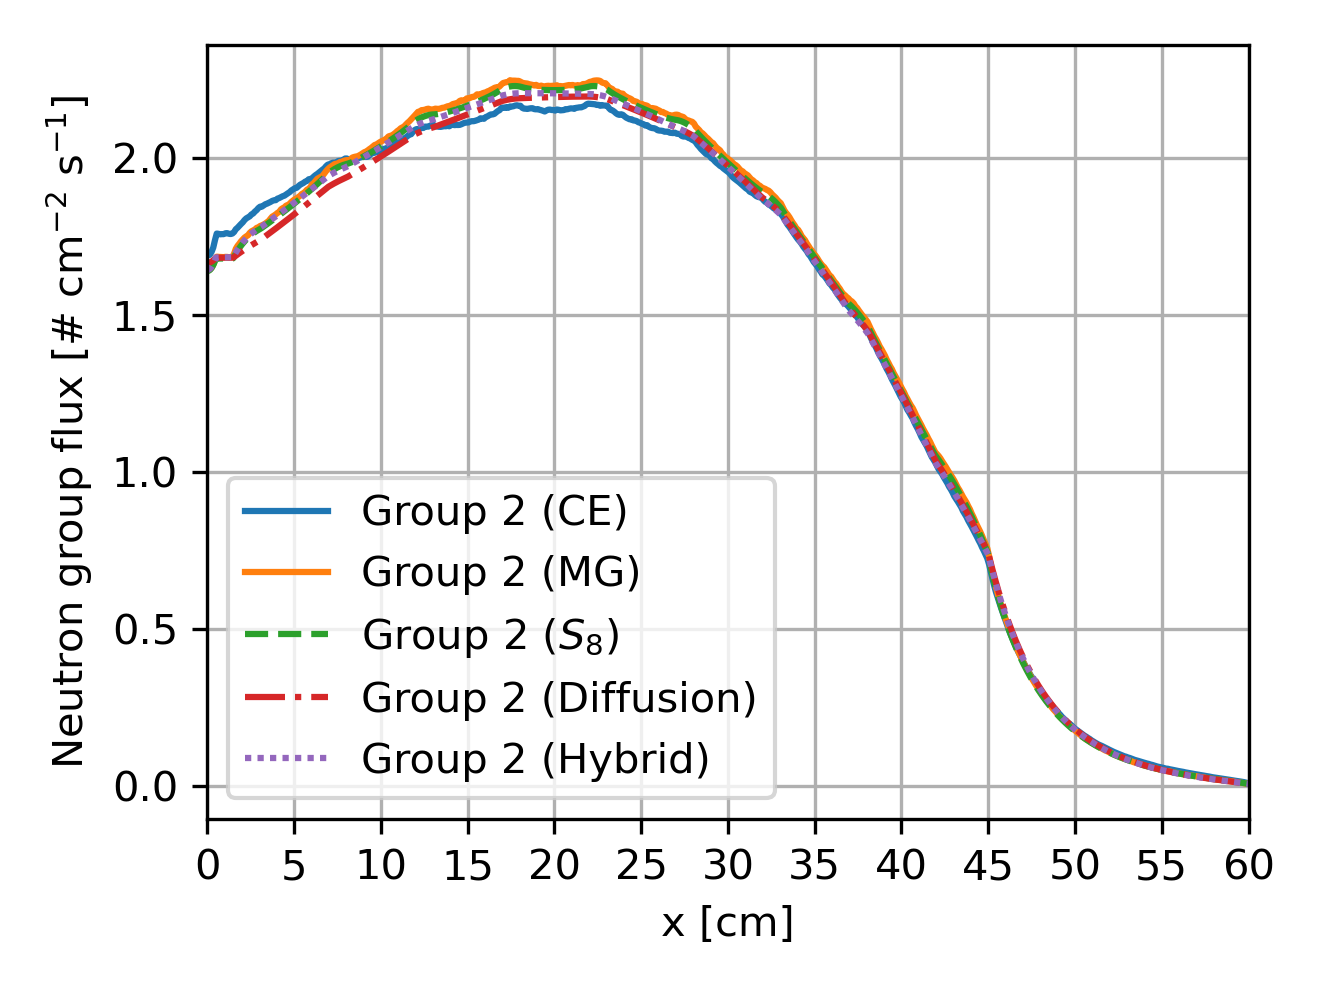
\includegraphics[width=\textwidth]{case-5a-group-2-flux}
    \caption{Group 2}
    \label{fig:c5ag2}
  \end{subfigure}
  \begin{subfigure}[t]{.49\textwidth}
    \centering
    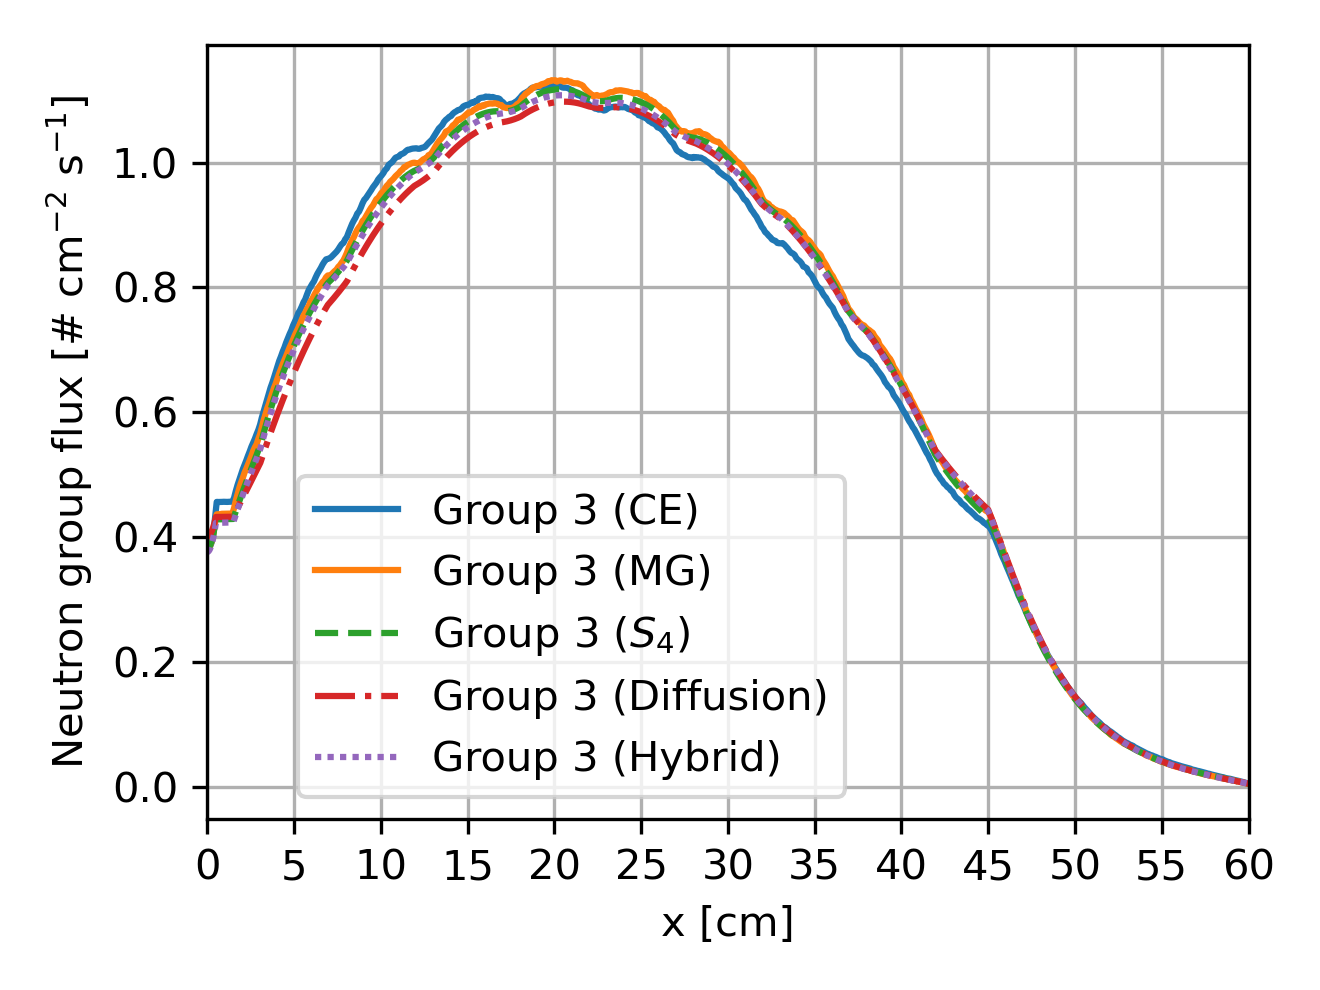
\includegraphics[width=\textwidth]{case-5a-group-3-flux}
    \caption{Group 3}
    \label{fig:c5ag3}
  \end{subfigure}
  \hfill
  \begin{subfigure}[t]{.49\textwidth}
    \centering
    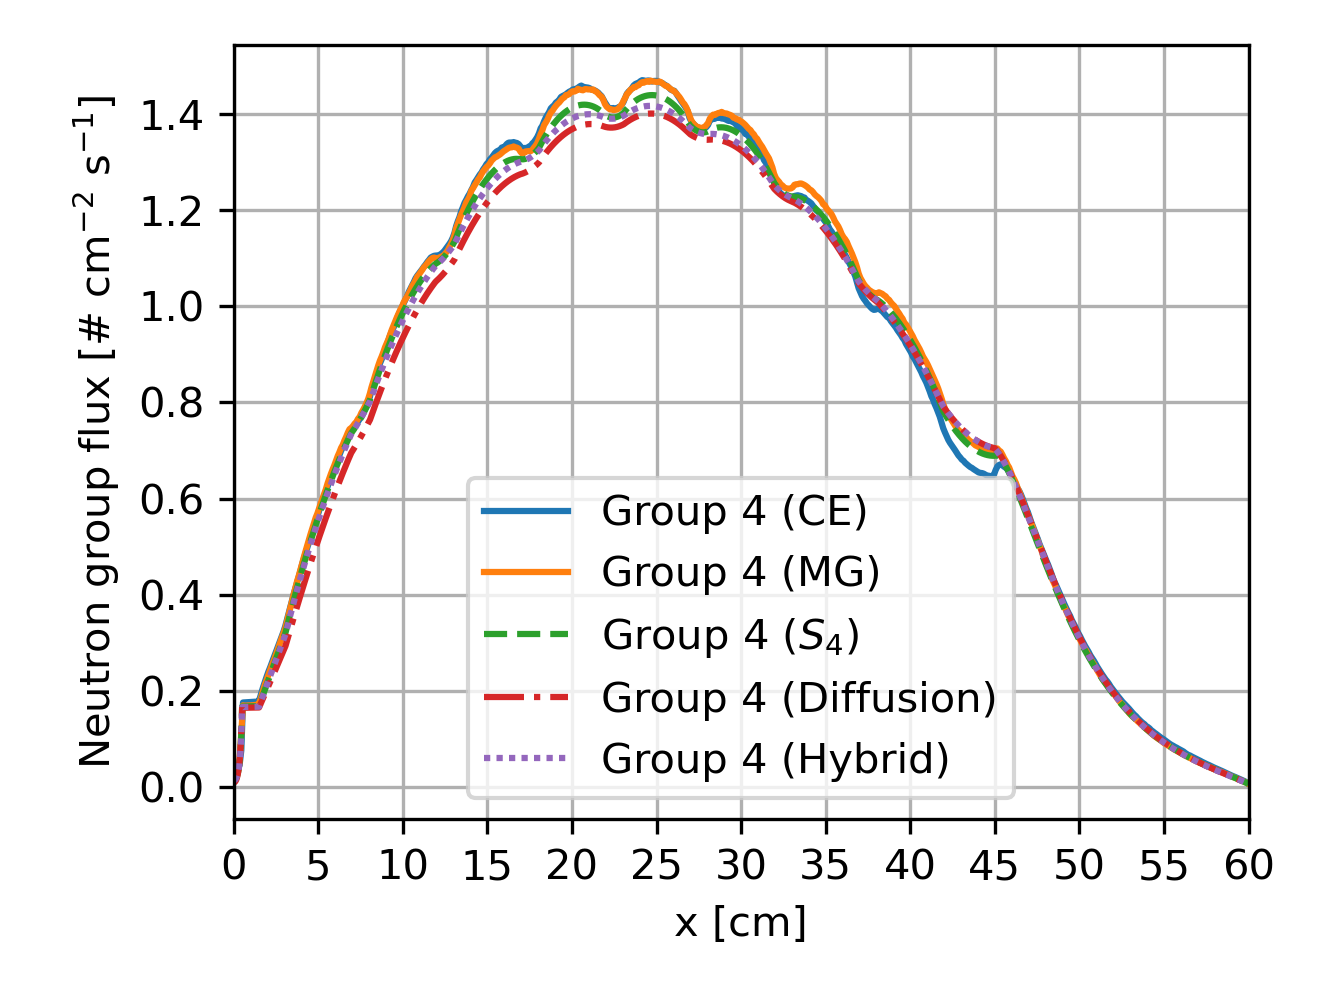
\includegraphics[width=\textwidth]{case-5a-group-4-flux}
    \caption{Group 4}
    \label{fig:c5ag4}
  \end{subfigure}
  \caption{Neutron group flux distributions for Case 5a from OpenMC-CE, OpenMC-MG, $S_8$, neutron
  diffusion, and hybrid methods.}
  \label{fig:c5aflux}
\end{figure}
%
\begin{figure}[htb!]
  \centering
  \begin{subfigure}[t]{.49\textwidth}
    \centering
    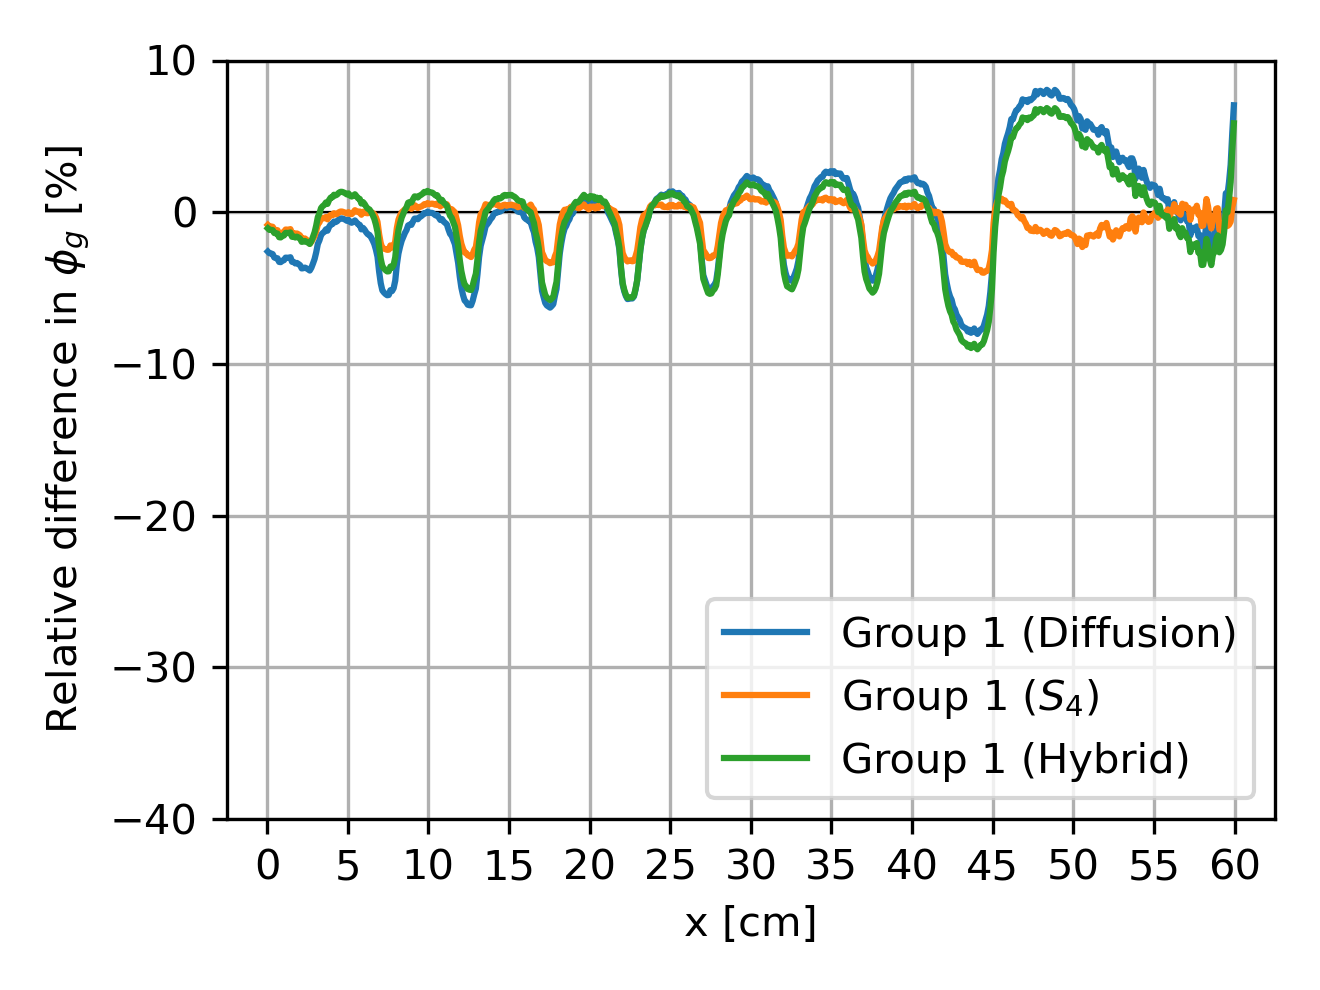
\includegraphics[width=\textwidth]{case-5a-group-1-flux-error}
    \caption{Group 1}
    \label{fig:c5ag1e}
  \end{subfigure}
  \hfill
  \begin{subfigure}[t]{.49\textwidth}
    \centering
    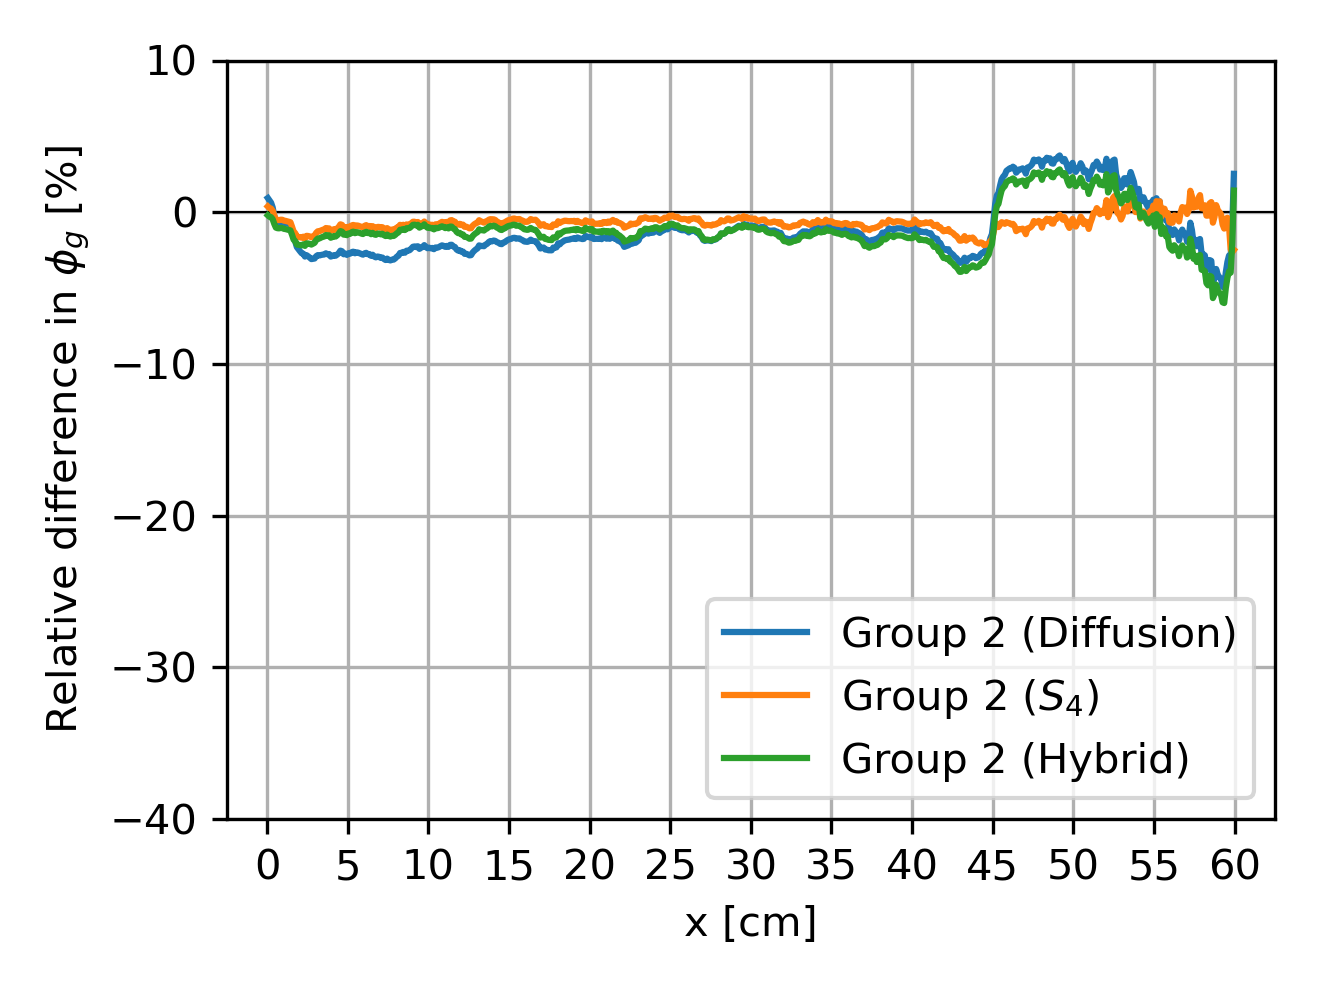
\includegraphics[width=\textwidth]{case-5a-group-2-flux-error}
    \caption{Group 2}
    \label{fig:c5ag2e}
  \end{subfigure}
  \begin{subfigure}[t]{.49\textwidth}
    \centering
    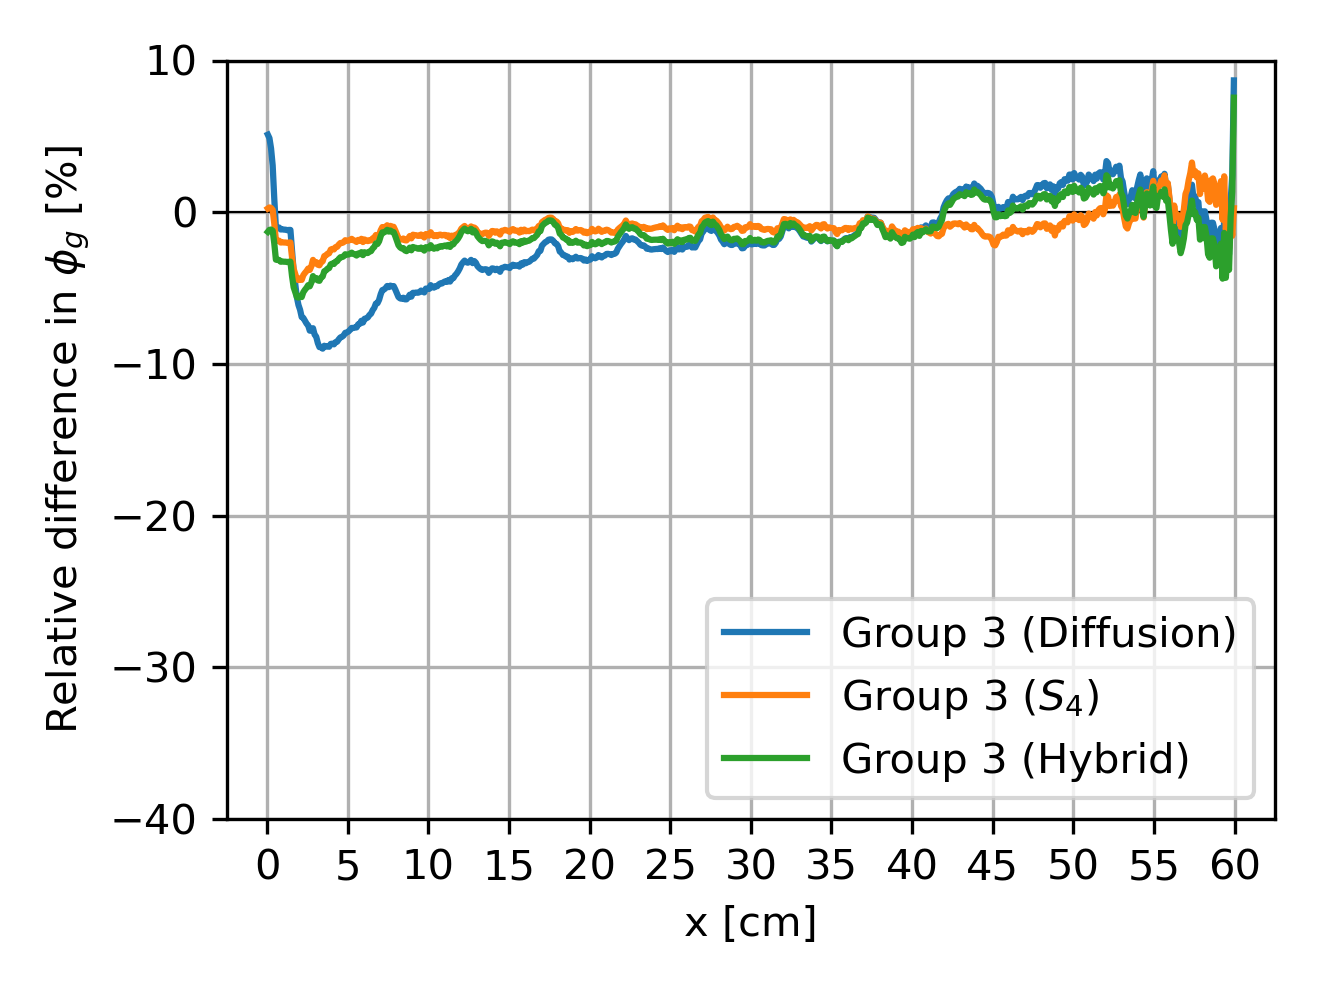
\includegraphics[width=\textwidth]{case-5a-group-3-flux-error}
    \caption{Group 3}
    \label{fig:c5ag3e}
  \end{subfigure}
  \hfill
  \begin{subfigure}[t]{.49\textwidth}
    \centering
    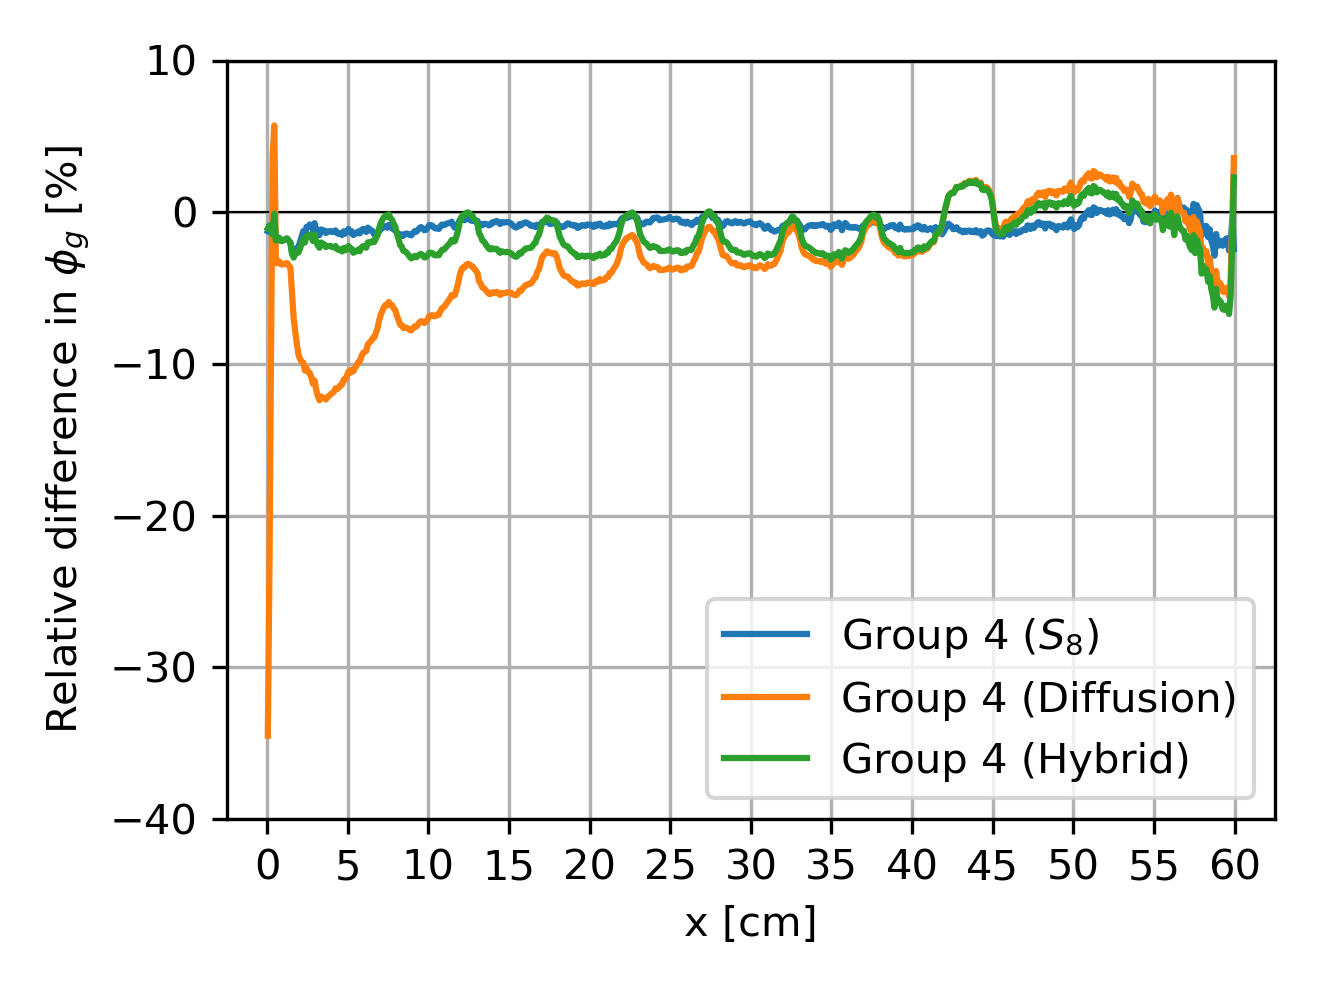
\includegraphics[width=\textwidth]{case-5a-group-4-flux-error}
    \caption{Group 4}
    \label{fig:c5ag4e}
  \end{subfigure}
  \caption{Relative differences of the neutron group flux distributions for Case 5a from the $S_8$,
    neutron diffusion, and hybrid methods with respect to OpenMC-MG.}
  \label{fig:c5afluxe}
\end{figure}
%
\begin{table}[tb!]
  \centering
  \footnotesize
  \caption{Normalized flux error $\varepsilon$ for Case 5a from the $S_8$, neutron diffusion, and
    hybrid methods with respect to OpenMC-MG.}
  \begin{tabular}{c S S S S}
    \toprule
    {\multirow{2}{*}{\textbf{Method}}} &
    \multicolumn{4}{c}{\textbf{Normalized flux error,} $\bm{\varepsilon_g}$} \\
    \cmidrule{2-5}
    & {\textbf{Group 1}} & {\textbf{Group 2}} & {\textbf{Group 3}} &
    {\textbf{Group 4}} \\
    \midrule
    $S_8$     & 0.0078 & 0.0074 & 0.0083 & 0.0085 \\
    Diffusion & 0.0305 & 0.0202 & 0.0313 & 0.0406 \\
    Hybrid    & 0.0290 & 0.0147 & 0.0143 & 0.0216 \\
    \bottomrule
  \end{tabular}
  \label{table:c5aerror}
\end{table}

\subsection{Correction Regions \& Diffusion Coefficients}

In this section, I compare the $P_1$-based diffusion coefficients, reference \glspl{SVDC}, and
hybrid \glspl{SVDC} for Cases 3b and 5a. As in Section \ref{sec:hybrid-method}, the reference
\glspl{SVDC} are derived from the $S_8$ flux solution, while the hybrid \glspl{SVDC} are derived
from the $S_8$ sub-solver flux solution within the hybrid $S_N$-diffusion method.

Figure \ref{fig:c3bdiffcoef} shows the various diffusion coefficient distributions for Case 3b
between $x=0$ cm and $x=30$ cm. The figures omit the large diffusion coefficient values in the
air gap region between $x=0.5$ cm and $x=1$ cm since they do not show any significant features. The
hybrid \glspl{SVDC} closely match
the reference \gls{SVDC} within most of the correction region, which terminates at $x=20$ cm.

\begin{figure}[htb!]
  \centering
  \begin{subfigure}[t]{.49\textwidth}
    \centering
    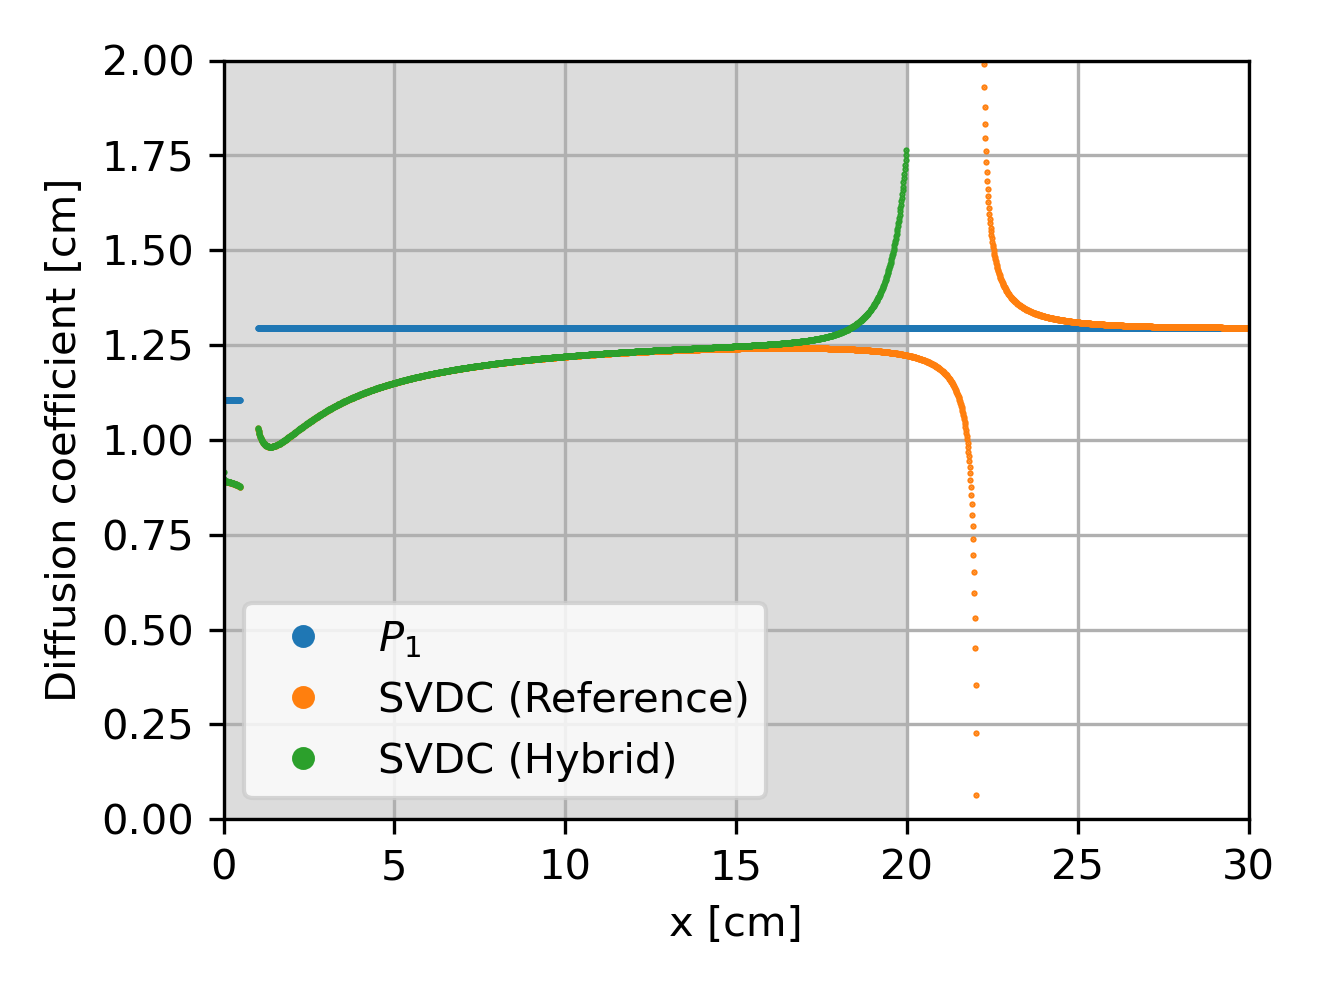
\includegraphics[width=\textwidth]{case-3b-group-1-diffcoef}
    \caption{Group 1}
    \label{fig:c3bg1dc}
  \end{subfigure}
  \hfill
  \begin{subfigure}[t]{.49\textwidth}
    \centering
    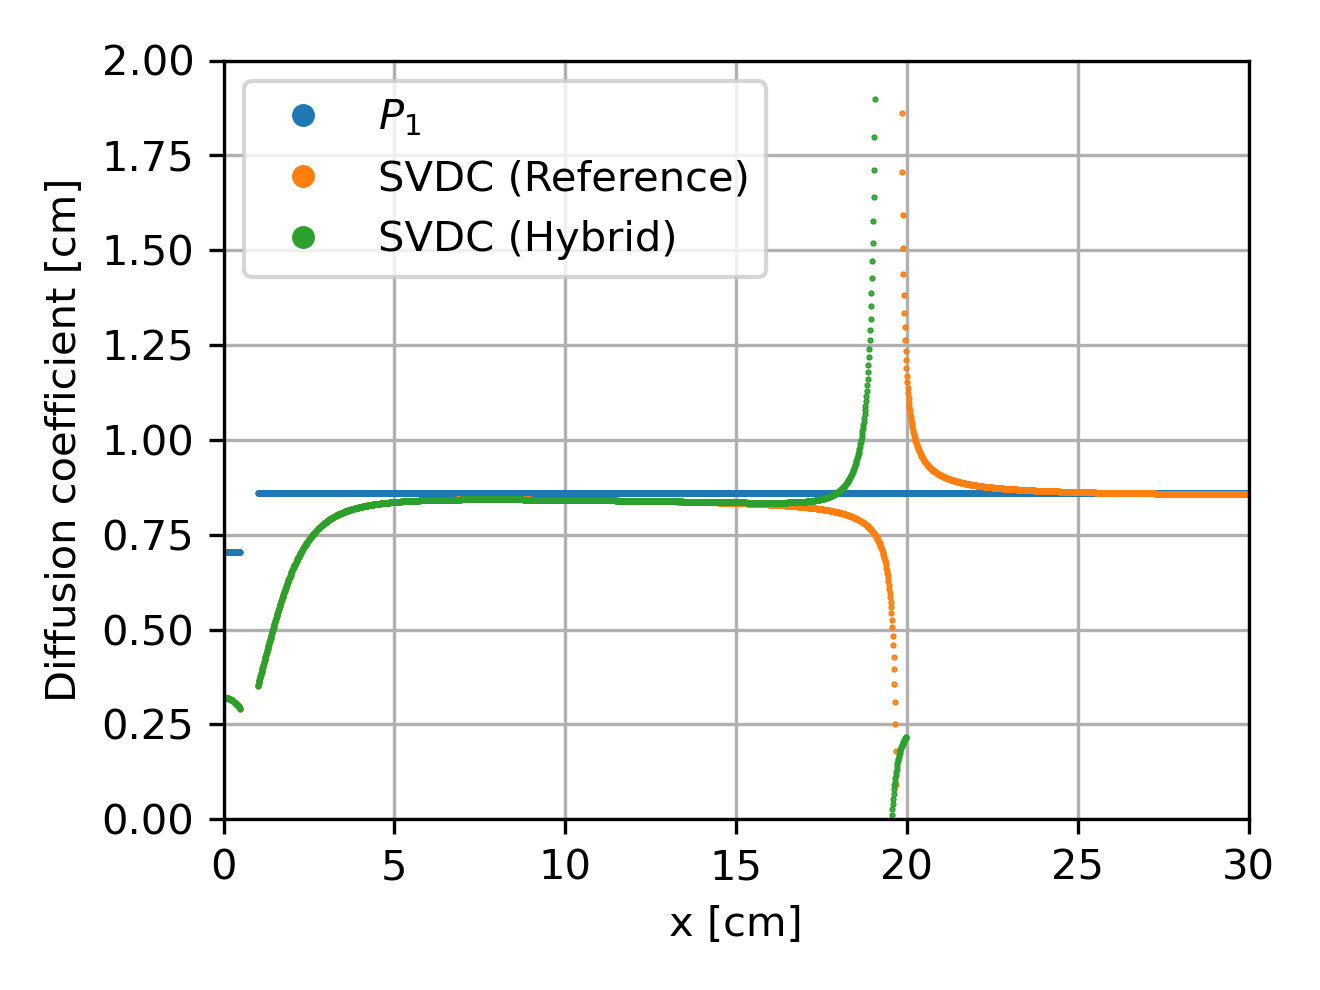
\includegraphics[width=\textwidth]{case-3b-group-2-diffcoef}
    \caption{Group 2}
    \label{fig:c3bg2dc}
  \end{subfigure}
  \begin{subfigure}[t]{.49\textwidth}
    \centering
    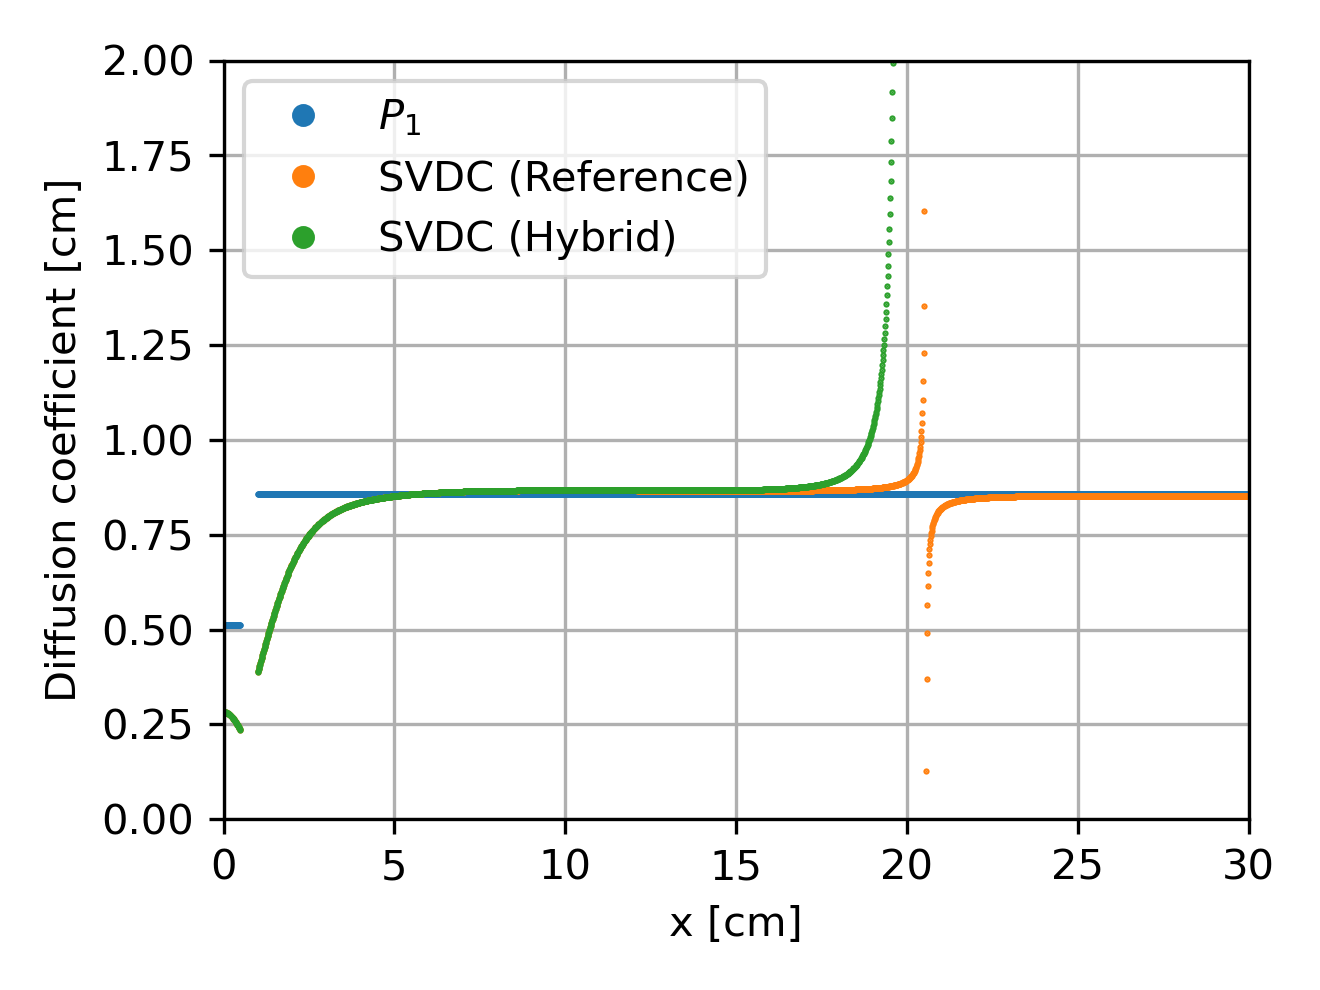
\includegraphics[width=\textwidth]{case-3b-group-3-diffcoef}
    \caption{Group 3}
    \label{fig:c3bg3dc}
  \end{subfigure}
  \hfill
  \begin{subfigure}[t]{.49\textwidth}
    \centering
    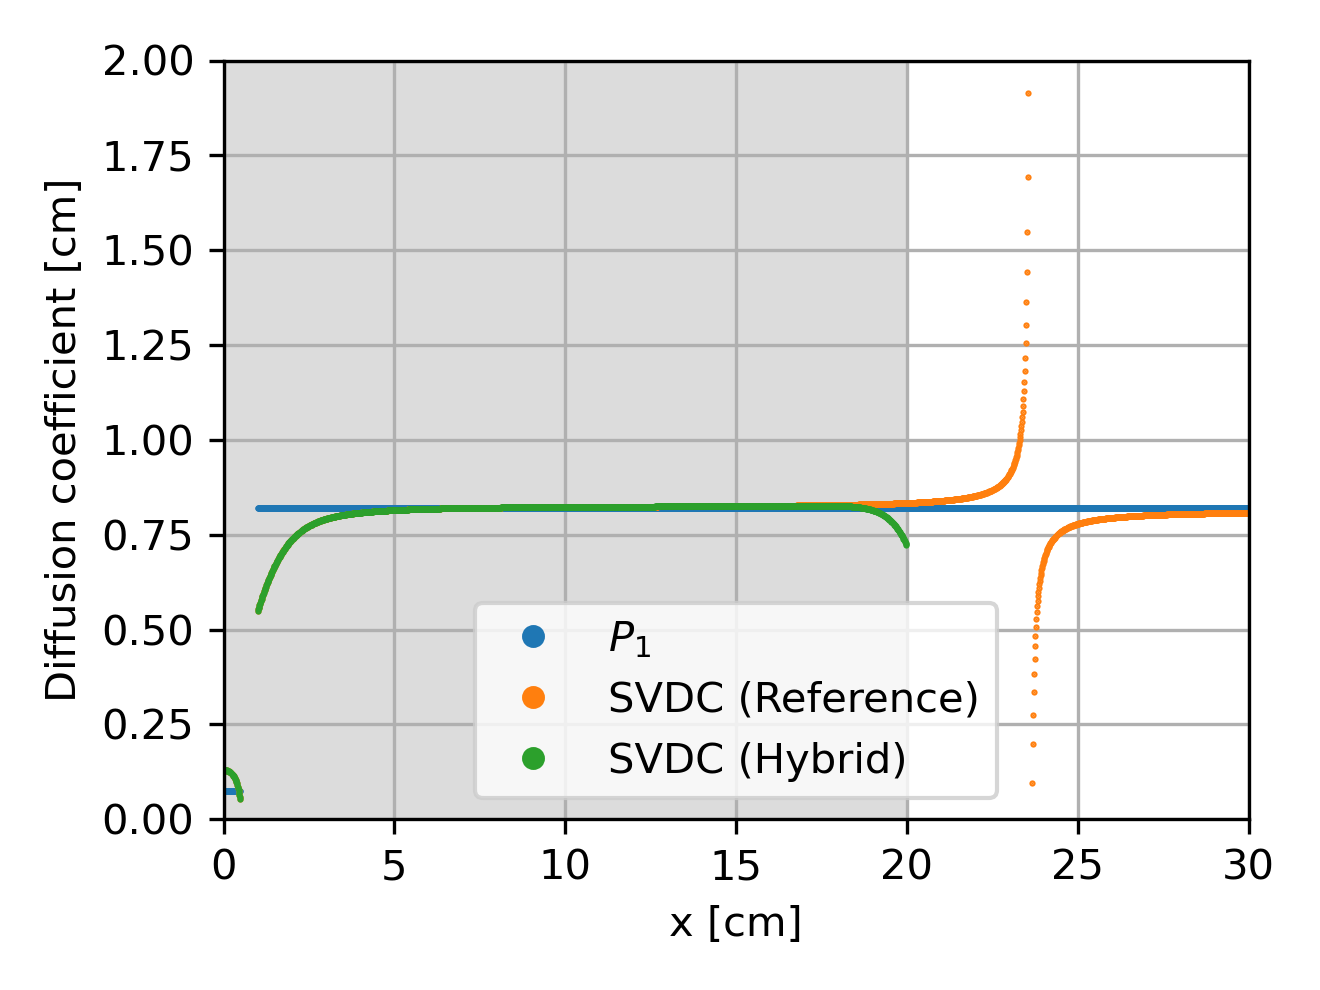
\includegraphics[width=\textwidth]{case-3b-group-4-diffcoef}
    \caption{Group 4}
    \label{fig:c3bg4dc}
  \end{subfigure}
  \caption{$P_1$-based diffusion coefficient, reference \gls{SVDC}, and hybrid \gls{SVDC}
    distributions for Case 3b between $x=0$ cm and $x=30$ cm.}
  \label{fig:c3bdiffcoef}
\end{figure}
%
\begin{figure}[htb!]
  \centering
  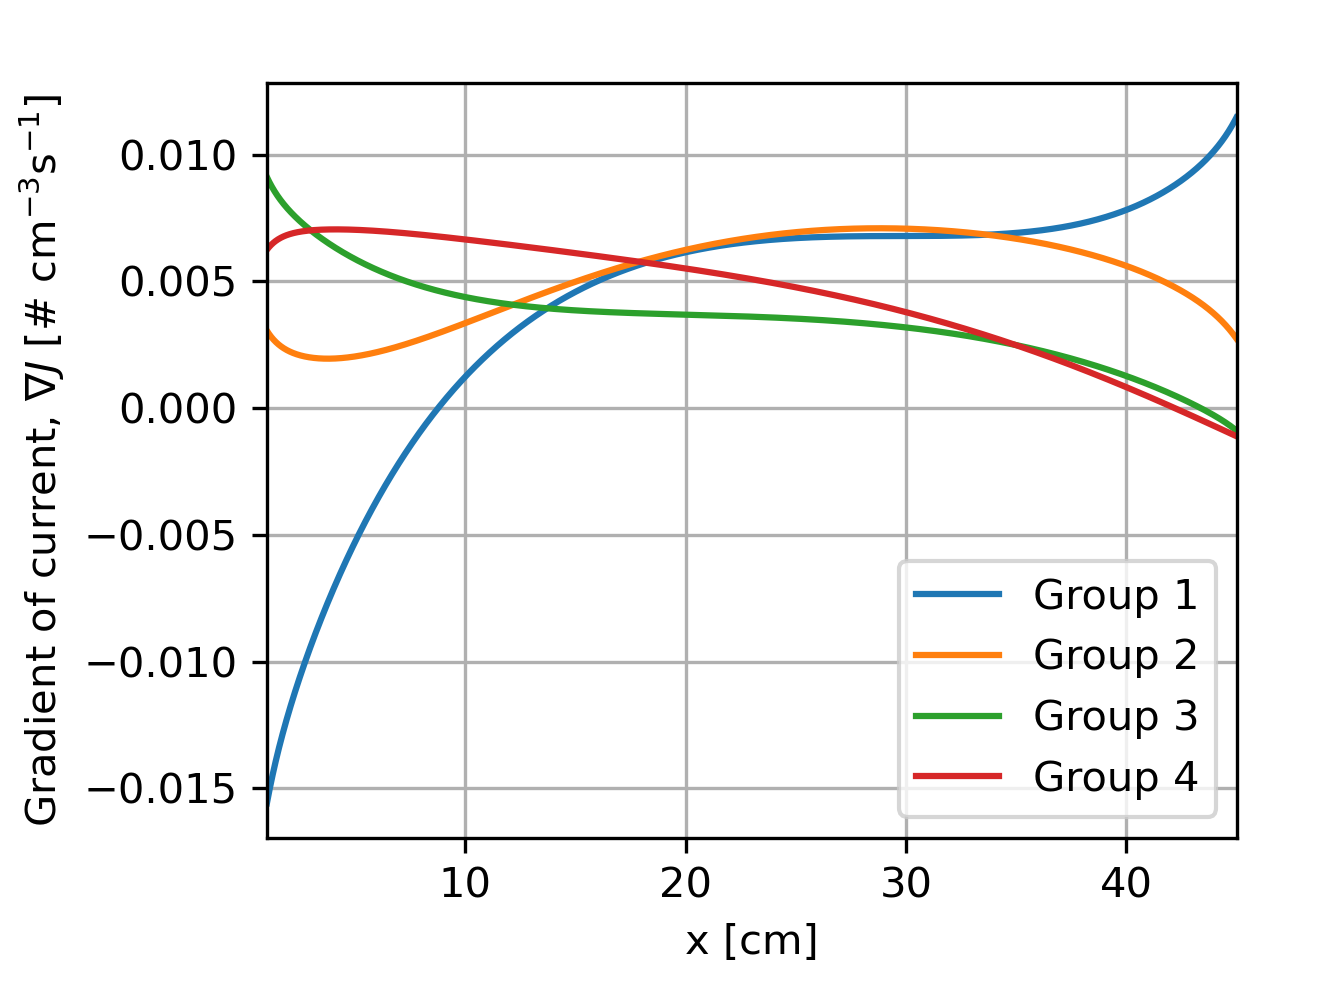
\includegraphics[width=.6\textwidth]{case-3b-grad-j}
  \caption{The gradient of current $J$ in the homogeneous fuel-graphite mixture from $x=1$ cm to
  $x=45$ cm for Case 3b.}
  \label{fig:c3bgradj}
\end{figure}

We recall that the hybrid method determines cutoff points within the correction region where the
\glspl{SVDC} coincide with the $P_1$-based diffusion coefficients so that the flux gradients
remain continuous. The hybrid method discards \glspl{SVDC} in the buffer region between this
cutoff point and the correction region boundary in favor of the $P_1$-based diffusion coefficients.
Notably, the group 1 reference \glspl{SVDC} (Figure \ref{fig:c3bg1dc}) only coincides
with the $P_1$-based diffusion coefficient after the vertical asymptotes where the flux
gradient approaches zero. The trends in group 1 reference \glspl{SVDC} before and after the
vertical asymptote imply that the \gls{SVDC} would have gradually approached the $P_1$-based
diffusion coefficient value if the asymptote did not exist. Determining the cutoff point for the
\glspl{SVDC} would have been problematic due to the vertical asymptote. However, the hybrid
\glspl{SVDC} coincide with the $P_1$-based diffusion coefficients before the vertical asymptote.
This behavior can be reliably reproduced in other geometries with large homogeneous fissile regions
(Cases 2a, 2b, and 3a) as long as the correction region terminates near the neutron flux peaks.
Nevertheless, the issue of handling vertical asymptotes in the \glspl{SVDC} has to be addressed
since flux peaks and troughs will inevitably occur in more realistic reactor geometries.

In contrast with the flux distributions in Figure \ref{fig:c3bflux}, the \gls{SVDC} distributions
suggest that the control rod contributes to an extended range of transport corrections on group 1
neutrons than the slower neutron groups. This phenomenon can be largely attributed to the highly
non-uniform fission neutron source distribution, which serves as the only source of group 1
neutrons in the absence of neutron up-scattering. The group 4 flux distribution
significantly influences on fission neutron source distribution, leading to more group 1 neutrons
being born closer to the reflector on the right than the
control rod on the left. The biased neutron source distribution induces a highly non-linear neutron
current distribution, as shown in Figure \ref{fig:c3bgradj}, and a departure from Fick's first law,
which relates the current to the flux gradient. Therefore, the \gls{SVDC} distributions show that
transport corrections to the faster neutron groups are as necessary for overall accuracy as
transport corrections to the slower neutron groups.

Figure \ref{fig:c5adiffcoef} shows the various diffusion coefficient distributions for Case 5a
between $x=0$ cm and $x=30$ cm. As with Case 3b, the figures omit the large diffusion coefficient
values in the air gap region between $x=0.5$ cm and $x=1.5$ cm  The hybrid \glspl{SVDC} closely match
the reference \gls{SVDC} within most of the correction region, which terminates at $x=10$ cm.

\begin{figure}[htb!]
  \centering
  \begin{subfigure}[t]{.49\textwidth}
    \centering
    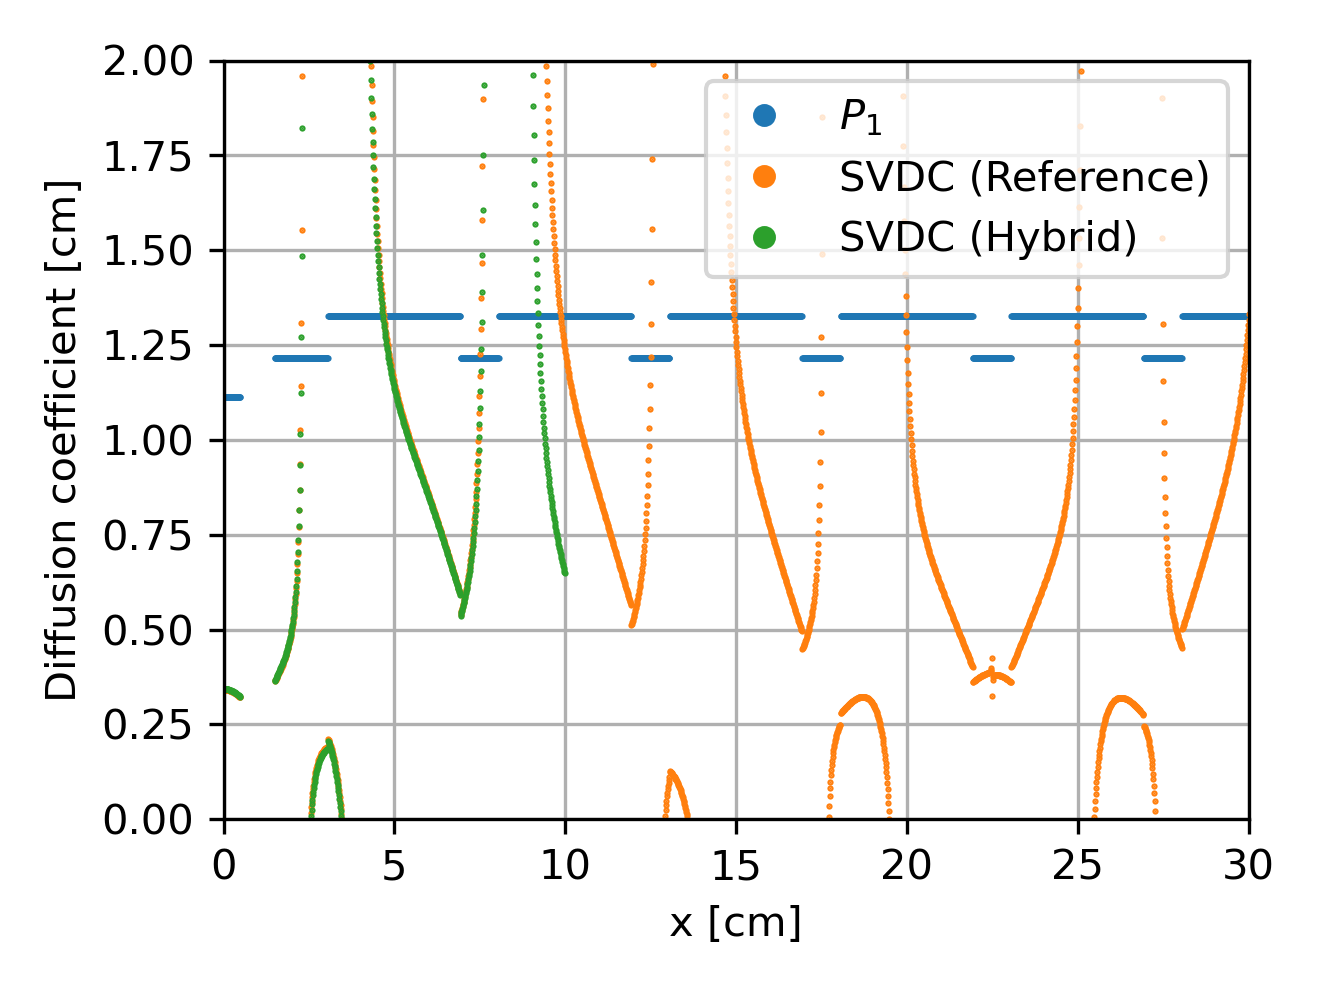
\includegraphics[width=\textwidth]{case-5a-group-1-diffcoef}
    \caption{Group 1}
    \label{fig:c5ag1dc}
  \end{subfigure}
  \hfill
  \begin{subfigure}[t]{.49\textwidth}
    \centering
    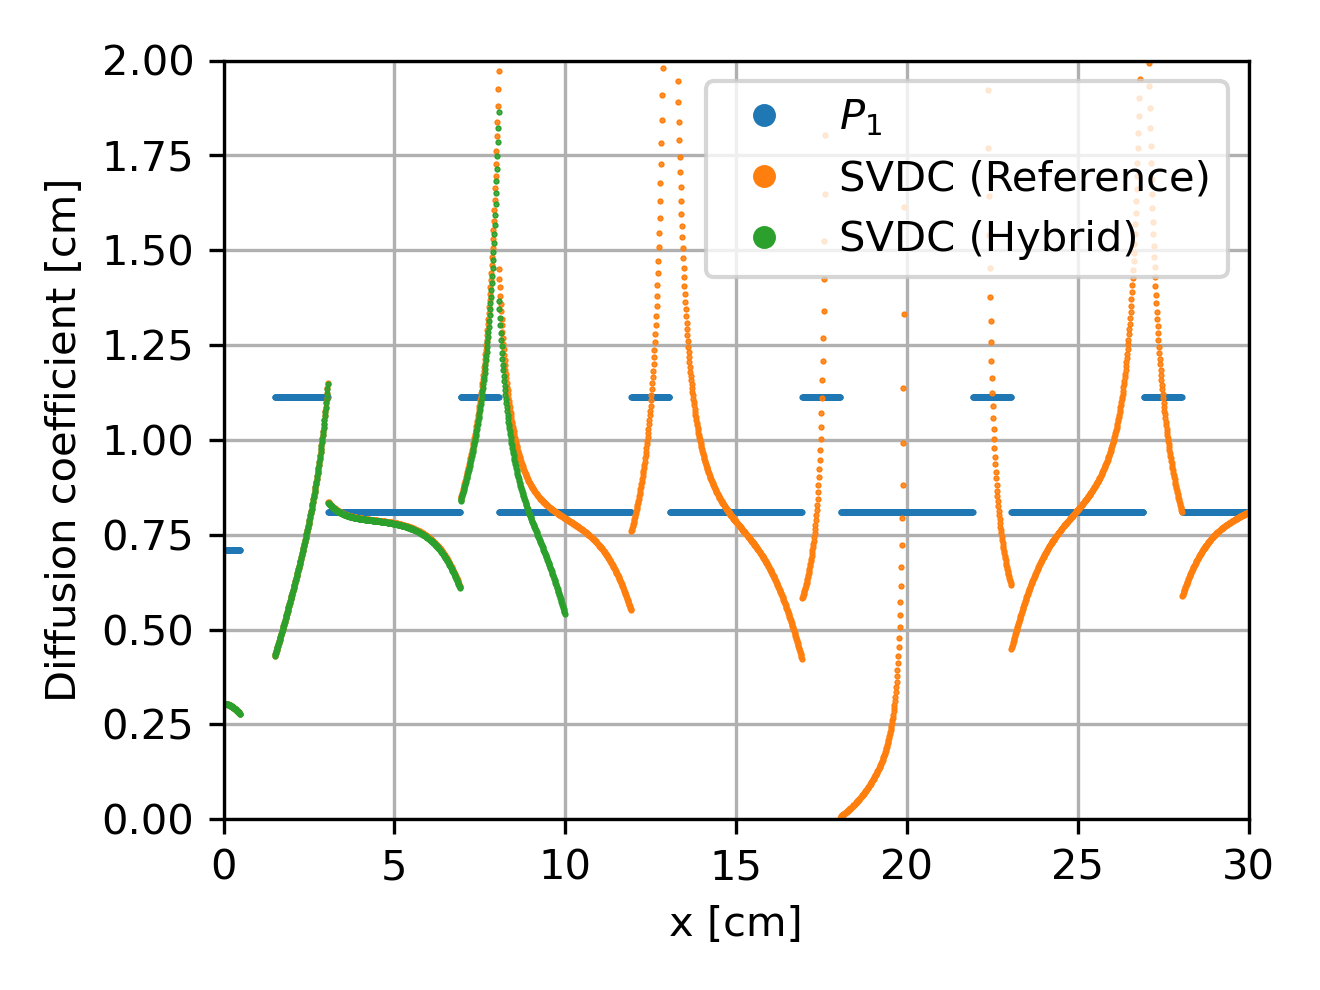
\includegraphics[width=\textwidth]{case-5a-group-2-diffcoef}
    \caption{Group 2}
    \label{fig:c5ag2dc}
  \end{subfigure}
  \begin{subfigure}[t]{.49\textwidth}
    \centering
    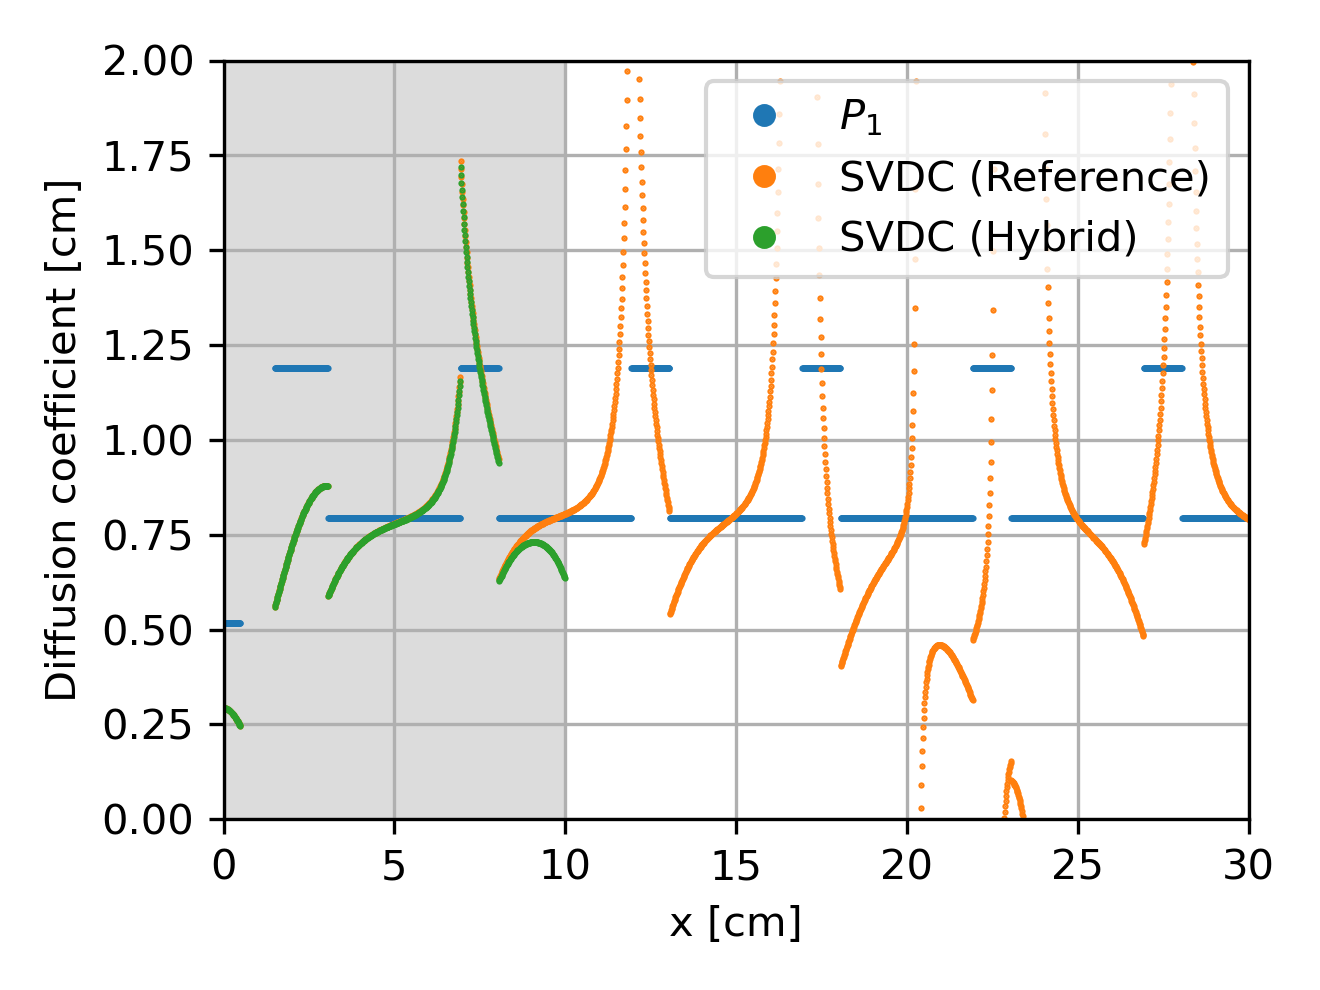
\includegraphics[width=\textwidth]{case-5a-group-3-diffcoef}
    \caption{Group 3}
    \label{fig:c5ag3dc}
  \end{subfigure}
  \hfill
  \begin{subfigure}[t]{.49\textwidth}
    \centering
    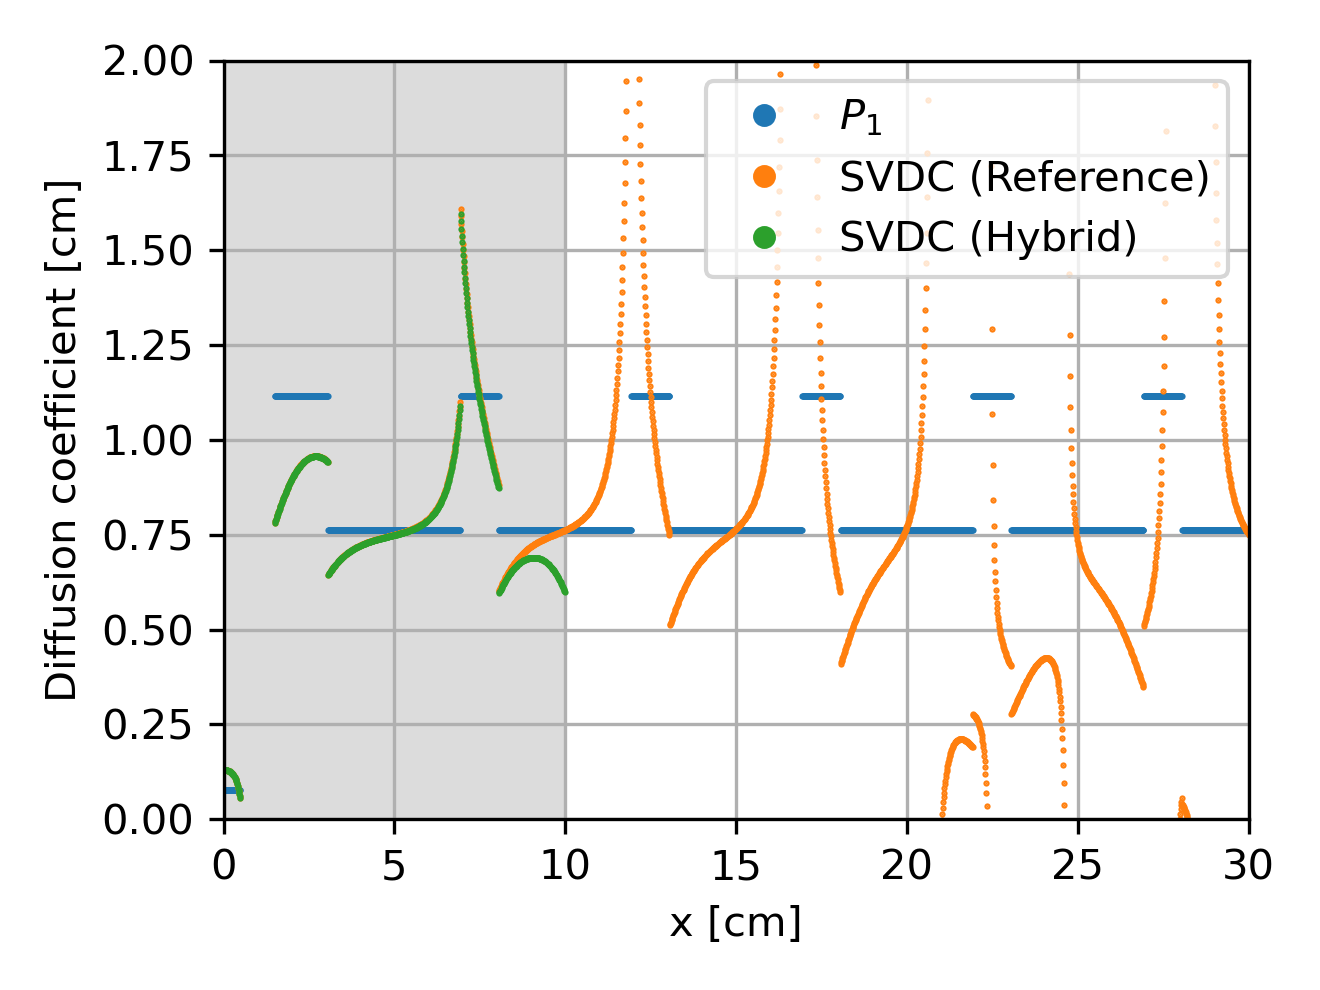
\includegraphics[width=\textwidth]{case-5a-group-4-diffcoef}
    \caption{Group 4}
    \label{fig:c5ag4dc}
  \end{subfigure}
  \caption{$P_1$-based diffusion coefficient, reference \gls{SVDC}, and hybrid \gls{SVDC}
    distributions for Case 5a between $x=0$ cm and $x=30$ cm.}
  \label{fig:c5adiffcoef}
\end{figure}

Unlike Case 3b, the heterogeneous fuel-graphite lattice structure in Case 5a gives rise to
extreme fluctuations in the \gls{SVDC} distributions. The numerous asymptotes correspond to the
flux peaks and troughs throughout the lattice. Regardless, the presence of the control rod
suppresses the \gls{SVDC} fluctuations in the lattice close to the control rod, and the cutoff
points can be determined without manual intervention. The heterogeneous lattice induces competing
effects on the neutron flux, allowing for a smaller correction region of 10 cm in width. However,
the reduced correction region introduces less transport correction as a consequence.
Further investigation is needed to observe how the \gls{SVDC} distributions change with
increases in dimensionality for 2-D and 3-D systems.

\section{Summary} \label{sec:hybrid-summary}

In this chapter, I presented the theoretical basis for a hybrid $S_N$-diffusion method, a novel
method for improving the neutron diffusion method for neutronics simulations of reactor
systems containing highly neutron-absorbing regions. The hybrid method relies on \glspl{SVDC}
derived from reference flux solutions of $S_N$ calculations to provide transport
corrections to the neutron diffusion method. The hybrid method is less computationally intensive
than the standalone $S_N$ neutron transport method because 1) $S_N$ calculations are limited to
correction regions which cover a fraction of the overall geometry, 2) and the \glspl{SVDC} are
observed to converge faster than the neutron fluxes in $S_N$ calculations.

I established a framework for the hybrid method for coupling an $S_N$ sub-solver and a neutron
diffusion solver through outer iterations by taking advantage of the weak dependence of the $S_N$
flux solution on the approximate boundary conditions determined from the neutron diffusion flux
solution. This framework could be extended to improve multischeme methods, which
divide a problem domain into subdomains where different neutronics methods are applied. For
instance, in an $S_N$-diffusion multischeme method, the $S_N$ method is applied in subdomains with
significant transport effects while other subdomains are treated with the neutron diffusion method
to reduce the overall computational effort required \cite{wang_rattlesnake_2021}. 

I also developed an algorithm for identifying and discarding inaccurate \gls{SVDC} values, which
are expected to occur near the correction region boundary. I demonstrated the hybrid
method on 1-D graphite-moderated test cases modeled after the \gls{MSRE}. The hybrid method showed
good agreement with the reference Monte Carlo and $S_8$ methods after eliminating neutron energy
group discretization errors in test cases that included highly neutron-absorbing regions. The
hybrid method had better accuracy in more homogeneous systems largely due to the larger effective
transport correction regions through \glspl{SVDC}. Further work
is needed to extend and verify the hybrid method to 2-D and 3-D neutronics simulations and to
create a robust solution for determining \glspl{SVDC} around neutron flux peaks and troughs. 
